% LaTeX source for book ``代数学方法'' in Chinese
% Copyright 2018  李文威 (Wen-Wei Li).
% Permission is granted to copy, distribute and/or modify this
% document under the terms of the Creative Commons
% Attribution 4.0 International (CC BY 4.0)
% http://creativecommons.org/licenses/by/4.0/

% To be included
\chapter{模论}\label{sec:modules}
模按纯量乘法的方式分成左右两种. 环 $R$ 上的左模 $M$ 粗看可以类比于向量空间, $M$ 本身对加法成群, 兼具 $R$ 的左纯量乘法 $R \times M \to M$. 从这个观点看, 向量空间是域上的模, 而交换群无非是 $\Z$-模.

模是数学中一种富于弹性, 用途特别广泛的结构; 例如
\begin{inparaenum}[(a)]
	\item 主理想环上的有限生成模结构定理涵摄了有限生成交换群的分类, 以及线性变换的标准形理论;
	\item 环 $R$ 上的模构成的范畴既是范畴论里的标准例子, 又是同调代数的原初样板;
	\item 模的张量积则为对称幺半范畴提供了极佳的例证.
\end{inparaenum}
本章探讨的正合列, 投射模与内射模理论如进一步发展, 就导向交换环论和同调代数; 而半单模和不可分解模的讨论则自然地通向群和代数的表示理论. 无论转向何方, 张量积都是必备工具, 也是初学模论的重点所在.

本章起将渐次增加范畴论的观点, 一方面固然是为了有效整理模的性质, 包括种种模范畴之间的函子, 与其间的自然变换, 另一方面也借此机会帮助读者熟悉范畴论的旨趣; 举凡伴随函子, 极限, 泛性质, 幺半范畴等概念都会在模论中找到合宜的位置, 表明这些抽象工夫既是自然的, 也是必要的.

\begin{wenxintishi}
	张量积是模论的关键之一, 为了囊括一般情形, 我们将铺陈双模情形下的一般理论; 相关表述因而显得复杂, 读者不妨先从交换环上的情形切入, 参见例 \ref{eg:bimodule-comm}. 我们将使用幺半范畴和幺半函子的语言表述张量积的诸般性质, 读者不必为此逐条审视范畴论里的相关定义, 但是对幺半范畴的精神应当有切实的认识: 幺半范畴是带有``张量积'' $\otimes$ 的范畴 + 种种约束同构, 而幺半函子是在自然同构意义下保持 $\otimes$ 的函子.
	
	本章关于正合列, 投射/内射模和链条件的讨论可视为走进交换环论和同调代数前的热身运动, 浅尝辄止. 适于考察这些概念的一般框架是 Abel 范畴; 环 $R$ 上的左模范畴就是 Abel 范畴的典型例子.
\end{wenxintishi}

\section{基本概念}
从形式观点看, 模是带有一族乘法算子的加法群. 回忆我们一贯的假设: 加法群意指交换群 $A$, 其二元运算记为 $+$, 幺元记为 $0$, 元素 $a \in A$ 的加法逆元记为 $-a$.

\begin{definition}\index{mo@模 (module)}
	设 $R$ 为环, 所谓的左 $R$-\emph{模}意谓以下资料:
	\begin{itemize}
		\item 加法群 $(M, +)$;
		\item 映射 $R \times M \to M$, 记为 $(r, m) \mapsto r \cdot m = rm$ (左乘), 满足以下性质:
		\begin{align*}
			r(m_1 + m_2) &= rm_1 + rm_2, \qquad r \in R, \; m_1, m_2 \in M, \\
			(r_1 + r_2)m &= r_1 m + r_2 m, \qquad r_1, r_2 \in R, \; m \in M, \\
			(r_1 r_2)m & = r_1 (r_2 m), \\
			1_R \cdot m & = m.
		\end{align*}
	\end{itemize}
	若将定义中的左乘改为右乘 $(m, r) \mapsto mr$, 条件改为 $m(r_1 r_2) = (mr_1)r_2$ 等等, 得到的概念称为右 $R$-模. 一般简称 $M$ 是左或右 $R$-模.
\end{definition}

比照熟悉的向量空间情形, 我们也称运算 $R \times M \to M$ 为 $R$ 的纯量乘法. 由以上公理容易导出在左 $R$-模 $M$ 中有下述性质
\begin{equation}\label{eqn:multiples-in-module}\begin{aligned}
	0 \cdot m & = 0, \quad m \in M, \\
	(-1_R) \cdot m & = -m, \\
	(n \cdot 1_R) \cdot m & = nm = \underbracket{m + \cdots + m}_{n\text{项}}, \quad n \in \Z_{\geq 0}, \\
	(-n \cdot 1_R) \cdot m & = -(nm).
\end{aligned}\end{equation}
因此形如 $n \cdot m$ ($n \in \Z$) 的表达式没有歧义: 既可视之为 $(M,+)$ 中的倍数运算, 亦可视为 $n \cdot 1_R \in R$ 的乘法作用. 右模的情形类似.

\begin{remark}\label{rem:module-multiplication}
	根据例 \ref{eg:End-ring}, 任意加法群 $(M, +)$ 的自同态集 $\End(M)$ 具备自然的环结构, 其乘法是同态的合成, 加法是同态的``逐点''加法. 赋予 $(M,+)$ 左 $R$-模结构相当于给定环同态
	\begin{align*}
		R & \longrightarrow \End(M) \\
		r & \longmapsto [m \mapsto rm],
	\end{align*}
	而赋予右 $R$-模结构相当于给定环同态
	\begin{align*}
		R^\text{op} & \longrightarrow \End(M) \\
		r & \longmapsto [m \mapsto mr].
	\end{align*}
	由此立得
	\begin{center}
		左 $R$-模 = 右 $R^\text{op}$-模.
	\end{center}
	交换环 $R$ 上的模不分左右, 可以简称为 $R$-模.
\end{remark}

\begin{example}
	任意环 $R$ 对自身的左乘法构成左 $R$-模, 对右乘法构成右 $R$-模.
\end{example}

\begin{example}\label{eg:Z-modules}
	整数环 $\Z$ 上的模无非是加法群, 这是由于 $\Z$ 在 $M$ 上仅有唯一一种乘法作用, 即 \eqref{eqn:multiples-in-module}. 所以交换群的理论可划为模论的一支.
\end{example}

\begin{definition}\label{def:submodule}\index{zimo@子模 (submodule)}
	设 $M$ 为左 $R$-模, 子集 $M' \subset M$ 如满足
	\begin{itemize}
		\item 加法封闭性: $M'$ 是加法群 $(M, +)$ 的子群,
		\item 纯量乘法封闭性: 对每个 $r \in R$, $m \in M'$ 皆有 $rm \in M'$,
	\end{itemize}
	则称 $M'$ 为 $M$ 的\emph{子模}. 右模的子模定义也是类似的.

	若左或右 $R$-模 $M$ 没有除了 $\{0\}$ 和 $M$ 自身之外的子模, 而且 $M \neq \{0\}$, 则称 $M$ 为\emph{单模}.\index{mo!单 (simple)}
\end{definition}

以下假设 $M$ 为左$R$-模. 令 $\{M_i: i \in I\}$ 为 $M$ 的一族子模, 则其和
\[ \sum_{i \in I} M_i := \left\{ 
	\begin{array}{ll}
		m_{i_1} + \cdots + m_{i_r} : & r \in \Z_{\geq 1}, \; i_1, \ldots, i_r \in I \\
		& \forall 1 \leq k \leq r, \; m_{i_k} \in M_{i_k}
	\end{array} \right\} \]
(约定空和为 $\{0\}$) 与交 (设 $I \neq \emptyset$)
\[ \bigcap_{i \in I} M_i \]
仍为子模. 令 $S$ 为 $M$ 的子集, 我们可以定义由 $S$ 生成的子模 $\lrangle{S}$ 为 $M$ 中包含 $S$ 的最小子模, 亦即
\[ \lrangle{S} := \bigcap_{\substack{M': \text{子模} \\ M' \supset S}} M'. \]
当 $S$ 是独点集 $\{x\}$ 时, $\lrangle{S} = \lrangle{x}$ 有直截了当的描述 $Rx := \{rx : r \in R\}$; 对于一般情形, 容易验证 $\lrangle{S} = \sum_{x \in S} Rx \subset M$. 能表成 $Rx$ 的形式的模称为\emph{循环模}; 当 $R=\Z$ 时, 循环模无非就是循环群.

对于右$R$-模可以依样画葫芦来定义子模 $xR$ 等等, 不再赘述.

\begin{example}
	环 $R$ 对本身的乘法具有自然的左模和右模结构. 比较子模和理想的定义 \ref{def:ideals} 可知
	\begin{center}
		$R$ 作为左 $R$-模的子模 = $R$ 的左理想, \\
		$R$ 作为右 $R$-模的子模 = $R$ 的右理想.
	\end{center}
	模论本身搭建在环的概念上, 以后将看到如何从 $R$-模观点反推 $R$ 的环论性质.
\end{example}

\begin{definition}\index{tongtai}
	设 $M_1$, $M_2$ 为左 $R$-模, 映射 $\varphi: M_1 \to M_2$ 若满足
	\begin{itemize}
		\item $\varphi$ 是加法群同态: 对所有 $x, y \in M_1$ 皆有 $\varphi(x+y)=\varphi(x) + \varphi(y)$,
		\item $\varphi$ 保持纯量乘法: 对所有 $r \in R$, $x \in M_1$ 皆有 $\varphi(rx) = r\varphi(x)$,
	\end{itemize}
	则称 $\varphi$ 为 $M_1$ 到 $M_2$ 的\emph{模同态}. 恒等映射显然是同态, 而同态 $\varphi: M_1 \to M_2$, $\psi: M_2 \to M_3$ 的合成 $\psi\varphi: M_1 \to M_3$ 仍为同态, 由此得到左 $R$-模的范畴 $R\dcate{Mod}$, 以及同构, 自同构等诸般概念. 右 $R$-模范畴的定义类似, 记为 $\cated{Mod}R$.\index{tonggou}

	对于如上的同态 $\varphi$, 定义其\emph{核}或曰零核为 $\Ker(\varphi) := \{x \in M_1 : \varphi(x)=0 \}$, 其\emph{像}为 $\Image(\varphi) := \{\varphi(x) : x \in M_1\}$, 两者分别是 $M_1$ 和 $M_2$ 的子模.\index{he}
\end{definition}

一如幺半群和环的情形, 同态 $\varphi: M_1 \to M_2$ 是同构当且仅当 $\varphi$ 是双射, 因为此时其逆映射 $\varphi^{-1}: M_2 \to M_1$ 也是模同态: 仅须对定义中 $\varphi$ 满足的等式取 $\varphi^{-1}$ 即可.

\begin{remark}\label{rem:Mod-cat-preadditive}
	与交换群或 $\Z$-模的状况相同, 对于任意左 (或右) $R$-模 $M, M'$, 同态集 $\Hom_{R\dcate{Mod}}(M, M') =: \Hom_R(M, M')$ 构成加法群: 对任意 $\phi, \psi \in \Hom_R(M, M')$, 定义
	\[ \phi + \psi := [m \mapsto \phi(m) + \psi(m) ] \in \Hom_R(M, M'). \]
	群 $\Hom_R(M, M')$ 的零元是\emph{零态射} $\forall m \mapsto 0$. 而且同态的合成运算
	\begin{align*}
		\Hom_R(M', M'') \times \Hom_R(M, M') & \longrightarrow \Hom_R(M, M'') \\
		(\phi, \psi) & \longmapsto \phi \psi
	\end{align*}
	是 $\Z$-双线性映射, 亦即:
	\[ \phi(\psi_1 + \psi_2) = \phi\psi_1 + \phi\psi_2, \quad (\phi_1 + \phi_2)\psi = \phi_1\psi + \phi_2\psi. \]

	由此亦可看出 $M$ 的自同态集 $\End_R(M)$ 具备自然的环结构, 乘法由合成给出. 以下且考虑右 $R$-模, 任意模 $M$ 于是获得自然的左 $D := \End_R(M)$-模结构如下
	\begin{align*}
		D \times M & \longrightarrow M \\
		(\phi, m) & \longmapsto \phi(m).
	\end{align*}
	这里的要点是 $D$ 的乘法作用与 $R$ 的作用相``交换'', 如 $\phi(mr)=\phi(m)r$. 我们尔后将见证这种结构的妙用, 见约定 \ref{con:Hom-assoc}, \ref{con:left-right-End}.
\end{remark}

根据注记 \ref{rem:module-multiplication}, 范畴 $R\dcate{Mod}$ 与 $\cated{Mod}R^\text{op}$ 等价. 为了省事, 以下固定环 $R$, 并且仅考虑左模的情形.

我们考虑模的商结构. 简言之, 给定左 $R$-模 $M$ 上一个``保持模结构''的等价关系 $\sim$ 相当于给定一个子模 $N$, 其间的联系是
\[ x \sim y \iff x-y \in N. \]
细节可参看 \ref{sec:homomorphism} 的讨论. 以下只说明如何从给定的子模 $N \subset M$ 构造商模 $M \twoheadrightarrow M/N$. 首先注意到作为加法群的商 $(M/N, +)$ 已有了定义, 其元素是形如 $x+N$ 的加法陪集, 二元运算是 $(x+N) + (y+N) = x+y + N$; 眼下任务是添上 $R$ 的纯量乘法.

\begin{definition}\index{shang}
	设 $N \subset M$ 为子模, 在加法商群 $M/N$ 上定义左 $R$-模结构
	\[ r (x+N) = rx + N, \qquad r \in R, \; x \in M. \]
	则商映射 $M \to M/N$ 是模同态, 称 $M/N$ 是 $M$ 对 $N$ 的\emph{商模}.
\end{definition}

商模满足与商群, 商环等类似的一些形式性质, 简要勾勒如次. 证明与群的情形类似, 而且由于不必考虑交换性, 其手法更为简单.

\begin{proposition}\label{prop:1st-homomorphism-module}
	商模 $M \twoheadrightarrow M/N$ 满足以下泛性质: 对任意模同态 $\varphi: M \to M'$, 若 $N \subset \Ker(\varphi)$, 则存在唯一的同态 $\bar{\varphi}: M/N \to M'$ 使得图表
	\[ \begin{tikzcd}
		M \arrow[rd, "\varphi"'] \arrow[r] & M/N \arrow[d, "{\exists! \; \bar{\varphi}}"]\\
		& M'
	\end{tikzcd}\]
	交换.
\end{proposition}
\begin{proof}
	唯一的取法是 $\bar{\varphi}(x + N) = \varphi(x)$, 易证此为良定的.
\end{proof}

\begin{proposition}\label{prop:quotient-image-module}
	设 $\varphi: M_1 \to M_2$ 是模同态, 则 $\varphi$ 诱导出同构 $\bar{\varphi}: M_1/\Ker(\varphi) \rightiso \Image(\varphi)$, 它映 $m + \Ker(\varphi)$ 为 $\varphi(m)$.
\end{proposition}
\begin{proof}
	应用命题 \ref{prop:1st-homomorphism-module}.
\end{proof}

\begin{proposition}\label{prop:2nd-homomorphism-module}
	设 $\varphi: M_1 \to M_2$ 是满的模同态. 则有双射
	\[ \begin{tikzcd}[row sep=tiny]
		\left\{ \text{子模 }  N_2 \subset M_2  \right\} \arrow[r, "1:1"] & \left\{ \text{子模 } N_1 \subset M_1 : N_1 \supset \Ker(\varphi)  \right\} \\
		N_2 \arrow[mapsto,r] & \varphi^{-1}(N_2) \\
		\varphi(N_1) & N_1 \arrow[mapsto, l].
	\end{tikzcd} \]
	此双射满足 $N_2 \subset N'_2 \iff \varphi^{-1}(N_2) \subset \varphi^{-1}(N'_2)$. 而且合成态射 $M_1 \xrightarrow{\varphi} M_2 \twoheadrightarrow M_2/N_2$ 诱导出同构 $M_1/\varphi^{-1}(N_2) \rightiso M_2/N_2$.
\end{proposition}
如取 $\varphi$ 为商同态 $M \twoheadrightarrow M/N$, 断言的同构可写成熟悉的形式 $M/N' \rightiso (M/N) \big/ (N'/N)$, 其中 $N \subset N'$.
\begin{proof}
	例行公事.
\end{proof}

\begin{proposition}\label{prop:3rd-homomorphism-module}
	设 $M, N$ 是 $\mathcal{M}$ 的子模, 合成同态 $M \hookrightarrow M+N \twoheadrightarrow (M + N)/N$ 诱导出自然的模同构
	\begin{align*}
		M/(M \cap N) & \rightiso (M+N)/N, \\
		m + (M \cap N) & \mapsto m + N, \quad m \in M.
	\end{align*}
\end{proposition}
\begin{proof}
	将商同态 $\pi: \mathcal{M} \to \mathcal{M}/N$ 限制到 $M$ 上, 其像显然为 $\pi(M) = M+N$, 核为 $M \cap \Ker(\pi) = M \cap N$. 应用命题 \ref{prop:quotient-image-module} 得到同构 $M/(M \cap N) \rightiso (M+N)/N$, 它映 $m + (M \cap N)$ 为 $m + N$.
\end{proof}

\begin{definition}\label{def:cokernel}
	对于模同态 $f: M \to M'$, 定义其\emph{余核}为 $\Coker(f) := M'/\Image(f)$.
\end{definition}
模范畴 $R\dcate{Mod}$ 的进一步性质将在 \S\ref{sec:exactseq-module} 予以探讨.

\section{模的基本操作}\label{sec:mod-operations}
本节取定环 $R$, 所论的模皆为左 $R$-模. 右模的情形是完全类似的.

\begin{definition}\label{def:tor-ann}
	设 $M$ 为 $R$-模.
	\begin{itemize}\index[sym1]{ann@$\text{ann}_M$}
		\item 元素 $x \in M$ 的\emph{零化子}定为 $R$ 的左理想如下
		\[ \text{ann}_M(x) := \{r \in R : rx=0 \}. \]
		若 $\text{ann}_M(x)=\{0\}$ 则称 $x$ 是\emph{无挠}的, 否则称之为\emph{挠元}, 所有非零元皆无挠的模称为\emph{无挠模}. \index{mo!无挠 (torsion-free)}
		\item 模 $M$ 的零化子定为 $R$ 的双边理想如下
		\[ \text{ann}(M) := \left\{r \in R: \forall x \in M, \; rx=0 \right\} = \bigcap_{x \in M} \text{ann}_M(x). \]
		若 $R$ 的双边理想 $I$ 包含于 $\text{ann}(M)$, 则 $M$ 自然地成为 $R/I$-模: 加法不变, 纯量乘法按 $(r + I)m = rm$ 来定义, 其中 $(r,m) \in R \times M$.
		\item 模 $M$ 对右理想 $\mathfrak{a} \subset R$ 的 $\mathfrak{a}$-\emph{挠部分}定为子模 \index[sym1]{$M[\mathfrak{a}]$}
		\[ M[\mathfrak{a}] := \left\{ m \in M: \forall a \in \mathfrak{a}, \; am=0 \right\}. \]
	\end{itemize}
\end{definition}
这些术语将在 \S\ref{sec:PID-module} 用到. 请读者验证 $M$ 作为 $R/\mathrm{ann}(M)$-模的零化子自动是 $\{0\}$.

本节的后续目标是以下定理. \index[sym1]{R-Mod@$R\dcate{Mod}$}
\begin{theorem}\label{prop:module-cat-completeness}
	范畴 $R\dcate{Mod}$ 是完备且余完备的, 并且具有零对象.
\end{theorem}

零对象是兼为始, 终对象的对象, 见定义 \ref{def:universal-objects}. 关于完备性及余完备性请参见定义 \ref{def:completeness}, 说穿了, $R$-模范畴具有所有小极限; 关于形容词``小''请参看定义 \ref{def:U-cat}. 关于 $\Z$-模即交换群的特例, 在例 \ref{eg:complete-cocomplete} 中已有勾勒. 以下证明将一并引入关于直和与直积的一些标准记法.

\begin{proof}
	注记 \ref{rem:Mod-cat-preadditive} 已说明了 $R\dcate{Mod}$ 是 $\cate{Ab}$-范畴: 这是说其中 $\Hom$-集有自然的加法群结构, 使得态射的合成是双线性的; 特别地, 对任意 $M$, $M'$ 存在零态射 $0: M \to M'$, 它将每个元素映到 $0$. 下面将循序渐进地构作各类极限.

	\begin{asparaenum}
		\item 范畴 $R\dcate{Mod}$ 的零对象是零模 $\{0\}$, 经常简记为 $0$. 其上的模结构只能是 $r \cdot 0 = 0$. 显然, 出入零模的态射恰好是零态射, 因此它确实是范畴 $R\dcate{Mod}$ 的零对象.

		\item 我们接着在 $R\dcate{Mod}$ 中构造积和余积. 设 $I$ 为小集, 而 $\{M_i : i \in I\}$ 为一族 $R$-模. 定义其\emph{积} (或称\emph{直积}) $\prod_{i \in I} M_i$ 为
		\begin{align*}
			\prod_{i \in I} M_i & := \left\{ (m_i)_{i \in I} : \forall i \in I, \; m_i \in M_i \right\}, \\
			(m_i)_{i \in I} + (m'_i)_{i \in I} & := (m_i + m'_i)_{i \in I}, \\
			r(m_i)_{i \in I} & := (rm_i)_{i \in I}, \quad r \in R.
		\end{align*}
		显然 $\prod_{i \in I} M_i$ 成 $R$-模, 其零元由 $\forall i \in I, \; m_i = 0$ 给出. 它带有一族投影同态
		\begin{align*}
			p_j: \prod_{i \in I} M_i & \longrightarrow M_j, \qquad j \in I \\
			(m_i)_{i \in I} & \longmapsto m_j.
		\end{align*}

		定义其\emph{余积} (惯称为\emph{直和}) 为 \index{zhihe@直和 (direct sum)}
		\begin{gather*}
			\bigoplus_{i \in I} M_i := \left\{ (m_i)_{i \in I} \in \prod_{i \in I} M_i : \text{仅至多有限个 } m_i \neq 0 \right\}
		\end{gather*}
		易见 $\bigoplus_{i \in I} M_i$ 为 $\prod_{i \in I} M_i$ 的子模. 它带有一族包含同态
		\begin{align*}
			\iota_j: M_j & \longrightarrow \prod_{i \in I} M_i \\
			m_j & \longmapsto (m_i)_{i \in I}, \quad m_i :=
			\begin{cases}
				m_j, & i=j, \\
				0, & i \neq j.
			\end{cases}
		\end{align*}

		若每个 $M_i = M$, 相应的直积与直和常写作 $M^I$ 和 $M^{\oplus I}$. 当 $I=\{1, \ldots, n\}$ 时我们常采用 $M_1 \times \cdots \times M_n$ 和 $M_1 \oplus \cdots \oplus M_n$ 的写法; 两者作为 $R$-模显然是一回事, 读者可进一步参看 \ref{def:biproduct} 关于双积的讨论. 我们回到一般的 $I$ 的情形, 接着验证 \S\ref{sec:limits} 中积和余积的范畴论性质.

		给定模 $M$ 和一族同态 $\phi_j: M \to M_j$, 我们希望存在唯一的 $\phi: M \to \prod_{i \in I} M_i$ 使得下图对每个 $j \in I$ 皆交换:
		\[ \begin{tikzcd}
			M \arrow[rd, "\phi_j"'] \arrow[r, "\phi"] & \prod_{i \in I} M_i \arrow[d, "p_j"] \\
			& M_j
		\end{tikzcd} \]
		此图定下了 $\phi(m)$ 的第 $j$ 个坐标, 因而唯一的取法显然是 $\phi(m) = (\phi_i(m))_{i \in I}$. 此即所求泛性质.

		类似地, 给定模 $M$ 和一族同态 $\psi_j: M_j \to M$, 使图表
		\[ \begin{tikzcd}
			\bigoplus_{i \in I} M_i \arrow[r, "\psi"] & M \\
			M_j \arrow[u, "\iota_j"] \arrow[ru, "\psi_j"'] &
		\end{tikzcd} \]
		对每个 $j \in I$ 交换的同态 $\psi$ 有唯一的取法: $\psi((m_i)_{i \in I}) = \sum_{i \in I} \psi_i(m_i)$ (有限和), 这是因为 $\bigoplus_{i \in I} M_i = \sum_{i \in I} \Image(\iota_i)$. 至此完成积和余积的构造.

		\item 下一步是在 $R\dcate{Mod}$ 中构造等化子和余等化子 (见 \S\ref{sec:limits}). 考虑一对同态 $f, g: X \to Y$. 等化子 $\Ker(f,g) \to X$ 的泛性质 \eqref{eqn:equalizer} 归结如下:
	    \begin{compactitem}
			\item 同态 $\iota: \Ker(f,g) \to X$ 满足 $f\iota = g\iota$;
			\item 假若 $\phi: L \to X$ 满足 $f\phi = g\phi$, 则存在唯一的分解 $\phi = [L \xrightarrow{\exists! \phi_0} \Ker(f,g) \xrightarrow{\iota} X]$.
		\end{compactitem}
		基于 $\Hom$ 集的加法群结构, 上述条件可以改写成 $(f-g)\iota = 0$, $(f-g)\phi = 0$, 因此构造 $\Ker(f,g) \to X$ 和构造 $\Ker(f-g, 0) \to X$ 是一回事. 我们立刻化约到 $g=0$ 的情形.

		准此要领, 观察余等化子 $Y \to \Coker(f,g)$ 的泛性质 \eqref{eqn:coequalizer}, 可知它无非是 $Y \to \Coker(f-g, 0)$. 同样化约到 $g=0$ 的情形.

		\item 现在描述等化子 $\Ker(f,0) \to X$, 其中 $f: X \to Y$ 是 $R$-模的同态. 泛性质化约为:
			\[ \left[ \phi: L \to X, \; f \phi = 0 \right] \implies \phi \; \text{有唯一的分解} \; L \to \Ker(f,0) \to X. \]
			注意到 $f\phi = 0 \iff \Image(\phi) \subset \Ker(f)$, 因此核 $\Ker(f) \hookrightarrow X$ 给出所求的等化子 $\Ker(f,0) \to X$.\index{denghuazi}

		\item 余等化子 $Y \to \Coker(f,0)$ 的情形类似, 其泛性质化约为:\index{yudenghuazi}
			\[ \left[ \psi: Y \to L, \; \psi f = 0 \right] \implies \psi \; \text{有唯一的分解} \; Y \to \Coker(f,0) \to L. \]
			由于 $\psi f = 0 \iff \Image(f) \subset \Ker(\psi)$, 应用命题 \ref{prop:1st-homomorphism-module} 可知余核 $Y \to \Coker(f) := Y/\Image(f)$ 给出所求的余等化子.
	\end{asparaenum}

	根据上述构造和推论 \ref{prop:completeness-criterion}, 范畴 $R\dcate{Mod}$ 具有所有的小极限.
\end{proof}

\begin{remark}\label{rem:filtrant-mod-limit}
	类似于集合情形, 模的滤过 $\varinjlim$ 具有更容易掌握的构造, 它涵摄了代数学中俗称的直极限. 设 $I$ 为滤过小范畴 (定义 \ref{def:filtrant-cat}) 并考虑函子 $\alpha: I \to R\dcate{Mod}$, 对象层面记作 $i \mapsto M_i$, 则 $\varinjlim_i M_i := \varinjlim \alpha$ 作为集合可以取为:
	\[ \varinjlim_i M_i := \left( \bigsqcup_{i \in \Obj(I)} M_i \right) \bigg/\sim \]
	其中 $\sim$ 是由 \eqref{eqn:filtrant-equiv} 定义的等价关系; 换句话说, 它是合成函子 $I \xrightarrow{\alpha} R\dcate{Mod} \to \cate{Set}$ 的 $\varinjlim$. 与环的情形 (命题 \ref{prop:ring-filtrant-limit}) 类似, 要点在于选取 $R$-模结构使得 $M_j \to \varinjlim_i M_i$ 成为同态, 选取既是明显的也是唯一的. 请读者仿照环的情形进行论证. 当 $I$ 是全序集而所有转移同态 $i \leq j \implies M_i \to M_j$ 都是单射时, 极限可以合理地写作 $\bigcup_i M_i$.
\end{remark}

举例明之, 任何模 $M$ 皆可表为它的有限生成子模的 $\varinjlim$, 这个极限是滤过的, 写法 $M = \bigcup_{\substack{N \subset M \\ \text{有限生成子模}}} N$ 也是自明的.

\begin{corollary}\label{prop:Mod-cat-additive}
	范畴 $R\dcate{Mod}$ 是加性范畴 (参看定义 \ref{def:additive-cat}). 特别地, $R$-模的有限直积与直和相等.
\end{corollary}
\begin{proof}
	定理 \ref{prop:module-cat-completeness} 构作了积和余积; 根据双积的定义 \ref{def:biproduct} 和定理 \ref{prop:biproduct-criterion} 可知这蕴涵双积存在性, 故 $\cate{Ab}$-范畴 $R\dcate{Mod}$ 实为加性范畴. 有限直积与直和的等同是命题 \ref{prop:additive-prod-coprod}, 按构造看亦属显然.
\end{proof}

\begin{lemma}\label{prop:prod-module}
	设环 $R$ 为直积 $R = \prod_{i \in I} R_i$, 其中 $I$ 是有限集. 对每个 $i \in I$ 定义 $R$ 的双边理想 $\mathfrak{b}_i := \prod_{\substack{j \in I \\ j \neq i}} R_j$, 以及
	\[ e_i := (\delta_{i,j})_{j \in I} \; \in R, \quad \delta_{i,j} = \begin{cases} 1, & i=j \\ 0, & i \neq j. \end{cases} \]
	对任意左 $R$-模 $M$ 定义 $M_i := \left\{ m \in M : \mathfrak{b}_i m = 0 \right\}$, 则有直和分解
	\begin{equation*}\begin{tikzcd}[row sep=tiny]
		\bigoplus_{i \in I} M_i \arrow[r, "\sim"] & M \\
		(m_i)_{i \in I} \arrow[mapsto, r] \arrow[phantom, u, "\in" description, sloped] & \sum_{i \in I} m_i \arrow[phantom, u, "\in" description, sloped] \\
		(e_i m)_{i \in I} & m \arrow[mapsto, l]
	\end{tikzcd}\end{equation*}
\end{lemma}
\begin{proof}
	运用性质 $\mathfrak{b}_i e_i = 0$, $\sum_i e_i = 1$ 和 $i \neq j \implies e_j \in \mathfrak{b}_i$ 来验证.
\end{proof}
在此亦可将 $M_i$ 视为 $R_i \simeq R/\mathfrak{b}_i$ 上的左模.
\begin{remark}
	反之, 给定一族左 $R_i$-模 $M_i$, 透过投影同态 $R \to R_i$ 将之拉回为左 $R$-模, 可构造直和 $M = \bigoplus_i M_i$. 容易验证两种构造在精确到自然同构的意义下互逆. 是以给定一个 $R$ 模相当于给定一族 $R_i$-模. 用范畴论的语言说, 我们得到 $R\dcate{Mod}$ 和 $\prod_{i \in I} (R_i\dcate{Mod})$ 间的范畴等价.
\end{remark}


\section{自由模}\label{sec:free-modules}
仍固定环 $R$. 接着考虑模范畴 $R\dcate{Mod}$ 中的``自由''构造. 设 $X$ 为(小)集合. 对每个 $x \in X$ 定义循环模 $Rx$ 如下: 其元素是形如 $rx$ 的符号, 其中 $r \in R$; 加法和纯量乘法分别定为 $rx + r'x = (r+r')x$, $r(r'x) = (rr')x$. 换言之, $Rx$ 其实就是作为左 $R$-模的 $R$, 只是形式地在右侧添上符号 $x$.
\begin{definition}\label{def:free-module}\index{mo!自由模 (free module)}
	以 $X$ 为基的\emph{自由模}定义为 $R^{\oplus X} = \bigoplus_{x \in X} Rx$. 作为集合有自然的包含映射
	\begin{align*}
		X & \longrightarrow R^{\oplus X} \\
		x & \longmapsto 1 \cdot x.
	\end{align*}
	其中的元素可以写成有限和 $m = \sum_{x \in X} a_x x$ 或数组 $(a_x)_{x \in X}$, 其中 $a_x \in R$ 是唯一确定的, 至多有限项非零; 这与定理 \ref{prop:module-cat-completeness} 证明中介绍的符号一致.
\end{definition}
这是自由模与基的外在定义, 稍后将给出内在版本. 易见 $X \mapsto R^{\oplus X}$ 定义函子 $\cate{Set} \to R\dcate{Mod}$, 它由以下泛性质刻画.

\begin{proposition}\label{prop:free-module-property}
	对任意 $R$-模 $M$ 和集合的映射 $\phi: X \to M$, 存在唯一的模同态 $\varphi: R^{\oplus X} \to M$ 使下图交换.
	\[ \begin{tikzcd}
		X \arrow[rd, "\phi"'] \arrow[r] & R^{\oplus X} \arrow[d, "{\exists! \, \varphi}"] \\
		& M
	\end{tikzcd} \]
\end{proposition}
\begin{proof}
	显然对每个 $x \in X$ 必须有 $\varphi(rx) = r\varphi(x) = r\phi(x) \in M$, 这就完全确定了 $\varphi$.
\end{proof}
因此函子 $X \mapsto R^{\oplus X}$ 是忘却函子的左伴随函子: 换言之, 存在自然同构
\[ \Hom_R(R^{\oplus X}, M) \rightiso \Hom_\cate{Set}(X, M), \]
其中的变元 $X$ 取遍集合而 $M$ 取遍 $R$-模. 换个观点看, 给出始于 $R^{\oplus X}$ 的同态相当于对基 $X$ 的每个元素指派其像, 不需任何约束条件, 因而是``自由''的.

借此机会, 我们将线性代数中几个常见的概念推广到模上.
\begin{definition}
	设 $X$ 为 $R$-模 $M$ 的子集. 根据命题 \ref{prop:free-module-property}, 包含映射 $X \hookrightarrow M$ 诱导出同态 $\sigma: R^{\oplus X} \to M$. 我们称
	\begin{itemize}
		\item $X$ 是\emph{线性无关}的或\emph{自由}的, 如果 $\sigma$ 是单射, 反之则称 $X$ 是\emph{线性相关}的;
		\item $X$ 生成或张成 $M$, 如果 $\sigma$ 是满射, 此时称 $X$ 为 $M$ 的\emph{生成集}. 具有有限生成集的模称为\emph{有限生成模}.\index{youxianshengcheng}
	\end{itemize}
	线性无关生成集称为\emph{基}; 具有基的模亦称\emph{自由模}, 这是定义 \ref{def:free-module} 的内禀版本.
\end{definition}
注意到 $\sigma$ 单等价于 $\Ker(\sigma)=\{0\}$, 这相当于说
\[ \underbracket{\sum_{x \in X} r_x x}_{M \text{中有限和}} = 0 \iff \forall x \in X, \; r_x = 0. \]
而 $\sigma$ 满等价于每个元素皆可表作 $R$-线性组合 $\sum_{x \in X} r_x x$. 这都是线性代数熟知的定义. 显然 $X$ 是$R^{\oplus X}$ 的基, 故自由模的内禀和外在定义是兼容的.

举例明之. 设 $\Delta$ 为幺半群, 读者可以验证定义 \ref{def:monoidal-ring} 构作的幺半群环 $R[\Delta]$ 对 $R$ 的左乘作用 $r\cdot(\sum_{\delta \in \Delta} r_\delta \delta) = \sum_{\delta \in \Delta} rr_\delta \delta$ (其中 $r \in R$) 构成左 $R$-模, 而且 $\Delta \subset R[\Delta]$ 是基. 右乘情形依此类推. 作为特例, 多项式环 $R[X] = \bigoplus_{n \geq 0 }RX^n$ 是以 $\Delta := \{ X^n: n \geq 0 \}$ 为基的自由左 $R$-模.

\begin{corollary}
	在同构意义下, 任意模 $M$ 皆可表成自由模的商.
\end{corollary}
\begin{proof}
	取 $M$ 的子集 $X$ 和相应的同态 $\sigma: R^{\oplus X} \to M$, 则 $\Image(\sigma) \simeq R^{\oplus X}/\Ker(\sigma)$. 如取 $X$ 为 $M$ 的生成集 (譬如 $X=M$), 则 $\Image(\sigma)=M$.
\end{proof}

当基 $X$ 有限时, $R^{\oplus X}$ 的自同态环可以表成熟悉的矩阵环形式, 见例 \ref{eg:matrix-ring}. 不失一般性设 $X = \{1, \ldots, n\}$. 我们先从 $\cated{Mod}R$ 中一般的有限积说起, 关键在于应用推论 \ref{prop:Mod-cat-additive}; 事实上以下论证适用于任意加性范畴 (定义 \ref{def:additive-cat}). 选定
\begin{compactitem}
	\item 正整数 $n, m$;
	\item 对象 $M_1, \ldots, M_n$ 和 $M'_1, \ldots, M'_m$.
\end{compactitem}
此处 $\bigoplus_{i=1}^n M_i$ 兼有直积直和两种角色, 分别由两族态射 $\bigoplus_{i=1}^n M_i \xrightarrow{p_j} M_j$ 和 $M_j \xrightarrow{\iota_j} \bigoplus_{i=1}^n M_i$ 给出. 同理有 $p'_j, \iota'_j$ 等态射. 于是根据积和余积的泛性质,
\begin{align*}
	\Hom \left( \bigoplus_{j=1}^n M_j, \bigoplus_{i=1}^m M'_i \right) & \xrightarrow[\sim]{\phi \mapsto (p'_i \phi)_i } \prod_{i=1}^m \Hom\left(\bigoplus_{j=1}^n M_j , M'_i \right) \\
	& \xrightarrow[\sim]{(p'_i \phi)_i \mapsto (p'_i \phi \iota_j)_{i, j}} \prod_{j=1}^n \prod_{i=1}^m  \Hom(M_j, M'_i).
\end{align*}
因此 $\phi: \bigoplus_{j=1}^n M_j \to \bigoplus_{i=1}^m M'_i$ 完全由同态族
\[ \phi_{ij} := p'_i \phi \iota_j: M_j \to M'_i, \quad 1 \leq i \leq m, \; 1 \leq j \leq n \]
确定, 表为矩阵
\[ \phi \longleftrightarrow \mathcal{M}(\phi) = (\phi_{ij})_{\substack{1 \leq i \leq m \\ 1 \leq j \leq n}} = \begin{pmatrix}
	\phi_{11} & \cdots & \phi_{1n} \\
	\vdots & \ddots & \vdots \\
	\phi_{m1} & \cdots & \phi_{mn} 
\end{pmatrix}. \]
回忆矩阵的乘法 $C=AB$ 由 $c_{ik} = \sum_j a_{ij} b_{jk}$ 确定. 对于矩阵 $\mathcal{M}(\phi)$, 尽管诸元取值在容或不同的 $\Hom$ (成加法群) 中, 下面涉及的运算仍是良定的.

\begin{lemma}\label{prop:Hom-matrix}
	对于 $\phi: \bigoplus_{i=1}^n M_i \to \bigoplus_{i=1}^{n'} M'_i$ 和 $\psi: \bigoplus_{i=1}^{n'} M'_i \to \bigoplus_{i=1}^{n''} M''_i$, 相应的矩阵满足
	\[ \mathcal{M}(\psi\phi) = \mathcal{M}(\psi) \mathcal{M}(\phi) \]
	其中矩阵元的相乘由合成 $\Hom(M_k, M'_j) \times \Hom(M'_j, M''_i) \to \Hom(M_k, M''_i)$ 给出.
\end{lemma}
\begin{proof}
	应用环 $\End_R(\bigoplus_i M'_i)$ 中的等式 $\sum_{j=1}^{n'} \iota'_j p'_j = 1$, $p'_i \iota'_i = \identity_{M'_i}$ 和 $i \neq j \implies p'_i \iota'_j = 0$ (双积定义 \ref{def:biproduct} 的多元版本) 计算 $\psi\phi$ 的第 $(i, k)$ 个矩阵系数 $\mathcal{M}(\psi\phi)_{ik}$: 根据同态合成的结合律与双线性, 可得
	\begin{align*}
		\mathcal{M}(\psi\phi)_{ik} = p''_i \psi\phi \iota_k & = \sum_{j=1}^{n'} p''_i \psi (\iota'_j p'_j) \phi \iota_k \\
		& = \sum_{j=1}^{n'} (p''_i \psi \iota'_j) (p'_j \phi \iota_k) = \sum_{j=1}^{n'} \mathcal{M}(\psi)_{ij} \mathcal{M}(\phi)_{jk}.
	\end{align*}
	这正是矩阵乘法. 断言得证.
\end{proof}

上述论证和线性代数中用矩阵表示线性变换的办法如出一辙.
\begin{proposition}\label{prop:End-matrix}
	模 $R^{\oplus n}$ 的自同态环自然地同构于 $n \times n$ 矩阵环 $M_n(R^\text{op})$, 此同构由 $\phi \mapsto \mathcal{M}(\phi)$ 导出. 进一步, 加法群 $\Hom_R(R^{\oplus n}, R^{\oplus m})$ 自然地同构于全体 $m \times n$ 矩阵的加法群 $M_{m \times n}(R^\text{op})$; 同态的合成对应到矩阵乘法.
	
	如改用右 $R$-模, 则相应地有 $\Hom_R(R^{\oplus n}, R^{\oplus m}) \simeq M_{m \times n}(R)$.
\end{proposition}
\begin{proof}
	视 $R$ 为左 $R$-模, 标作 ${}_R R$. 任意 $\phi \in \End({}_R R)$ 皆满足 $\phi(r) = r\phi(1)$, 由此可证
	\begin{align*}
		\End({}_R R) & \longrightarrow R^\text{op} \\
		\phi & \longmapsto \phi(1)
	\end{align*}
	是环同构: 其逆将 $r \in R$ 映至右乘自同态 $x \mapsto xr$ (留意到乘法顺序将倒转). 在先前的讨论和引理 \ref{prop:Hom-matrix} 中代入 $M_i = M'_j = {}_R R$, 即得所求. 对于右模则有 $\End(R_R) \simeq R$, 其余相同.
\end{proof}

下述``生成引理''涉及 \S\ref{sec:cardinal-number} 简介的无穷基数.
\begin{lemma}\label{prop:generator-cardinal}
	设 $I$ 为无穷集, $(M_i)_{i \in I}$ 为一族非零模, 则 $\bigoplus_{i \in I} M_i$ 的任意生成集 $S$ 皆满足 $|S| \geq |I|$.
\end{lemma}
\begin{proof}
	任意 $s \in S$ 可写成 $(s_i)_{i \in I}$, 记 $E_s := \{i \in I: s_i \neq 0\}$. 根据直和定义 $E_s$ 有限, 而 $S$ 生成 $\bigoplus_{i \in I} M_i$ 蕴涵了 $\bigcup_{s \in S} E_s = I$, 因之 $S$ 无穷. 推论 \ref{prop:cardinal-max} 遂蕴涵基数不等式
	\[ \max\{|S|, \aleph_0 \} = |S| \cdot \aleph_0 \geq \left| \bigcup_{s \in S} E_s \right| = |I|, \]
	而最左端无非是 $|S|$.
\end{proof}

最后来探讨自由模的秩. 以下设 $R$ 非零. 自然的想法是定 $M \simeq R^{\oplus X}$ 的秩为 $|X|$, 然而须说明这和基 $X \subset M$ 的选择无关. 当 $R$ 为域时, 向量空间的理论说明秩确实是良定的, 读者应已熟知有限维情形, 而定义--定理 \ref{def:dimension-vector-space} 将给出一般的证明, 引理 \ref{prop:generator-cardinal} 会派上用场. 由此可以推得交换环上的自由模也具有类似性质.

\begin{proposition}
	设 $R$ 为交换环, 则 $R^{\oplus X} \simeq R^{\oplus Y}$ 当且仅当 $|X|=|Y|$.
\end{proposition}
\begin{proof}
	显然 $|X|=|Y|$ 蕴涵 $R^{\oplus X} \simeq R^{\oplus Y}$. 为证明另一个方向, 我们应用命题 \ref{prop:existence-maximal-ideal} 取 $R$ 的一个极大理想 $\mathfrak{m}$. 对任意 $R$-模 $M$, 定义 $\mathfrak{m} M$ 为形如 $am$ ($m \in M$, $a \in \mathfrak{m}$) 的元素生成的子模. 于是 $M/\mathfrak{m}M$ 是 $R/\mathfrak{m}$-模, 亦即域 $R/\mathfrak{m}$ 上的向量空间. 当 $M = R^{\oplus X}$ 时易见 $\mathfrak{m}M = \mathfrak{m}^{\oplus X}$, 故有向量空间的同构
	\begin{align*}
	M/\mathfrak{m}M & \stackrel{\sim}{\longrightarrow} (R/\mathfrak{m})^{\oplus X} \\
	(a_x)_{x \in X} + \mathfrak{m}M & \longmapsto (a_x + \mathfrak{m})_{x \in X}.
	\end{align*}
	故 $|X| = \dim_{R/\mathfrak{m}} (M/\mathfrak{m}M)$, 等式右边只和 $M$ 的 $R$-模结构有关, 不依赖基的选取.
\end{proof}

\begin{definition}[自由模的秩]\label{def:rank-module}\index[sym1]{rank@$\rank_R(E)$}\index{zhi@秩 (rank)}
	设 $E$ 为非零交换环 $R$ 上的自由模, 其\emph{秩}定义为 $\rank_R(E) := |X|$, 如果 $E \simeq R^{\oplus X}$. 根据前述命题, 这是良定的.
\end{definition}

\begin{remark}\label{rem:IBN}
	对于一般的环 $R$, 如果 $I$ 为无穷集, $R^{\oplus I} \simeq R^{\oplus J}$, 则引理 \ref{prop:generator-cardinal} 蕴涵 $|J| \geq |I|$, 由对称性故 $|I|=|J|$. 因此环 $R$ 上的自由模有良定的秩当且仅当
	\[ \forall n,m \in \Z_{\geq 0}, \; R^{\oplus n} \simeq R^{\oplus m} \iff n=m. \]
	称此为左\emph{不变基数}性质 (英文简写为 IBN); 若考虑右模则谓右不变基数性质. 除环, 交换环和有限环皆有不变基数性质. 进一步的讨论可参看 \cite[\S 1]{Lam99}.
\end{remark}

\section{向量空间}\label{sec:vector-space}
读者理应接触过向量空间的理论. 从代数观点看, 向量空间大致是一种带有加法和纯量乘法的结构, 纯量乘法一般来自实数域 $\R$ 或复数域 $\CC$, 然而向量空间的代数性质实则可以建立在任意域上. 我们还能进一步舍弃乘法交换性, 进而考虑除环上的向量空间. 这既是一种自然又轻松的推广, 对于环论的研究也是必要的.

\begin{definition}\index{xiangliangkongjian@向量空间 (vector space)}
	设 $D$ 为除环. 我们称右 $D$-模为 $D$-向量空间. 其子模, 商模等也称为子空间, 商空间.
\end{definition}
定义中选取左模或右模其实无关宏旨, 当 $D$ 为域时更可以不论左右. 这里选取右乘主要是为了符号的方便: 若 $\varphi: V \to V'$ 为 $D$-向量空间的态射 (亦即右 $D$-模的态射), 则态射对纯量乘法的性质可以写成类似结合律的形式:
\[ \varphi (vd) = (\varphi v)d, \quad v \in V, \; d \in D. \]

以下选定除环 $D$. 子空间, 基和维数等概念可以毫不费力地推广到 $D$-向量空间上.

\begin{definition-theorem}\index{ji@基 (basis)}
	设 $V$ 为 $D$-向量空间, $X \subset V$, 以下性质等价:
	\begin{enumerate}[(i)]
		\item $X$ 是 $V$ 的极大线性无关子集;
		\item 包含映射 $X \hookrightarrow V$ 诱导出同构 $D^{\oplus X} \rightiso V$;
		\item $X$ 是 $V$ 的极小生成集;
		\item $V$ 中的任意元素皆可表成形如 $\sum_{x \in X} x d_x$ 的有限和, 其中 $(d_x)_{x \in X}$ 是唯一的.
	\end{enumerate}
	满足以上任一性质的 $X$ 称为 $V$ 的\emph{基}.
\end{definition-theorem}
\begin{proof}
	(i) $\implies$ (ii): 给定 $v \in V$, 由 $X$ 的极大性知 $X \sqcup \{v\}$ 必线性相关, 从而存在等式 $\sum_{x \in X \sqcup \{v\}} x d_x = 0$, 其中 $d_x$ 不全为零; 由 $X$ 的线性无关性可知 $d_v \neq 0$, 因此 $v = -\sum_{x \in X} x d_x d_v^{-1}$ 属于 $D^{\oplus X} \to V$ 的像. 既然 $D^{\oplus X} \to V$ 是单射, 它实为同构.

	(ii) $\implies$ (iii): 不妨设 $V = D^{\oplus X}$. 显然 $X$ 生成 $V$; 假若 $X' \subset X \smallsetminus \{y\}$ (其中 $y \in X$), 则 $y$ 显然不属于 $X'$ 生成的子模 $D^{\oplus X'}$, 因而 $X$ 是极小生成集.

	(iii) $\implies$ (iv): 由 $X$ 生成 $V$ 可知任意元素皆可表成有限和 $\sum_{x \in X} x d_x$. 假若
	\[ \sum_{x \in X} x d_x = \sum_{x \in X} x d'_x, \quad \exists y \in X, \; d_y \neq d'_y, \]
	则 $y = -\sum_{x \neq y} x (d_x - d'_x)(d_y - d'_y)^{-1}$, 由此导出 $X \smallsetminus \{y\}$ 也生成 $V$, 矛盾.

	(iv) $\implies$ (i): 子集 $X$ 显然线性无关. 任意 $v \in V$ 可表为 $\sum_{x \in X} x d_x$, 亦即 $v - \sum_{x \in X} x d_x = 0$, 是以 $X \sqcup \{v\}$ 线性相关.
\end{proof}

\begin{proposition}\label{prop:existence-basis}
	任意 $V$ 中的线性无关子集 $X$ 皆包含于某个基 $B$; 特别地, $V$ 有基.
\end{proposition}
\begin{proof}
	选定 $X$, 令 $\mathcal{E} := \{Y \subset V: \text{线性无关}, \; Y \supset X  \}$, 赋 $\mathcal{E}$ 以偏序 $Y \leq Y' \iff Y \subset Y'$. 今将运用 Zorn 引理 (定理 \ref{prop:Zorn}) 证明偏序集 $(\mathcal{E}, \leq)$ 有极大元, 从而得到所求之基: 仅须证明 $(\mathcal{E}, \leq)$ 中任意链 $\mathcal{E}'$ 有上界即可. 令 $Y \subset V$ 为 $\mathcal{E}'$ 中所有元素之并, 我们断言 $Y$ 线性无关: 假设等式
	\[ \sum_{y \in Y} y d_y = 0 \quad \text{(有限和)} \]
	成立, 由于 $\mathcal{E}'$ 为全序, 可取充分大的 $Y_0 \in \mathcal{E}'$ 使得 $y \notin Y_0 \implies d_y = 0$; 再利用 $Y_0$ 的线性无关性质, 即可导出$\forall y \in Y, \; d_y = 0$. 此 $Y$ 即为所求上界.
\end{proof}

\begin{lemma}[Steinitz 换元性质]\label{prop:exchange-vector-space}
	设 $X$, $Y$ 为 $V$ 的两组有限基, $y \in Y \smallsetminus X$, 则存在 $x \in X \smallsetminus Y$ 使得 $(Y \smallsetminus \{y\}) \cup \{x\}$ 为基.
\end{lemma}
\begin{proof}
	留意到 $X$ 非空确保 $Y$ 非空. 每个 $x \in X$ 可唯一地展为 $Y$ 的 $D$-线性组合, 我们断言 $y$ 必须出现在某个 $x$ 的展式中, 否则 $Y \smallsetminus \{y\}$ 将是 $V$ 的一组生成元, 与基的定义矛盾. 取如是 $x$ 并定义 $Z := (Y \smallsetminus \{y\}) \cup \{x\}$. 观察到
	\begin{inparaenum}[(a)]
		\item 每个 $Y$ 中元素都能展成 $Z$ 的线性组合, 考虑 $y$ 的情形并利用 $x$ 的展式即可;
		\item $Z$ 必线性无关: 否则因为 $Y \smallsetminus \{y\}$ 线性无关故, $x$ 必能表成 $Y \smallsetminus \{y\}$ 的线性组合, 回忆上一步可知 $y$ 也能表成 $Y \smallsetminus \{y\}$ 的线性组合, 矛盾.
	\end{inparaenum}
	于是 $V$ 中元素能唯一地表成 $Z$ 的线性组合. 最后观察到 $x \notin Y$: 设若不然, 则 $y \notin X \implies y \neq x \implies Z = Y \smallsetminus \{y\}$, 与基是极大线性无关子集这一性质矛盾.
\end{proof}

换元性质是证明维数良定的关键. 由于类似论证在代数学中并非孤例, 在此乘势引入一套组合学的工具.
\begin{definition}[H.\ Whitney]\label{def:matroid}\index{nizhen@拟阵 (matroid)}
	设 $E$ 为集合, $\text{Bs}$ 为 $E$ 的一族有限子集; 如下列条件满足则称资料 $(E, \text{Bs})$ 为\emph{拟阵}:
	\begin{enumerate}[\bfseries {B}.1]
		\item 集合 $\text{Bs}$ 非空;
		\item 若 $X, Y \in \text{Bs}$ 而 $y \in Y \smallsetminus X$, 则存在 $x \in X \smallsetminus Y$ 使得 $(Y \smallsetminus \{y\}) \cup \{x\}\; \in \text{Bs}$.
	\end{enumerate}
\end{definition}
举例来说, 只要 $D$-向量空间 $V$ 有一组有限基, 那么引理 \ref{prop:generator-cardinal} 蕴涵每个基皆有限, 这时运用引理 \ref{prop:exchange-vector-space}, 取 $E := V$ 和 $\text{Bs} := \{ V\;\text{的基} \}$ 便给出拟阵. 一般定义中还要求 $E$ 有限, 不过这点在此无关宏旨. 拟阵的奥妙在于它有种种等价然而面貌迥异的刻画, 感兴趣的读者可参阅专著 \cite{Oxl11}. 

\begin{proposition}\label{prop:matroid-rank}
	设 $(E, \mathrm{Bs})$ 为拟阵, 则 $\mathrm{Bs}$ 的每个元素都有相同的基数; 此基数称为该拟阵的秩.
\end{proposition}
\begin{proof}
	设若不然, 取 $X, Y \in \text{Bs}$ 使得 $|Y| > |X|$ 且 $|Y \smallsetminus X|$ 尽可能小; 前一条件保证 $Y \smallsetminus X \neq \emptyset$. 根据换元性质 (\textbf{B.2}) 可取 $y \in Y \smallsetminus X$ 和 $x \in X \smallsetminus Y$ 使得 $Y' := (Y \smallsetminus \{y\}) \cup \{x\}\; \in \text{Bs}$. 从 $|Y|=|Y'| > |X|$ 和 $|Y' \smallsetminus X| < |Y \smallsetminus X|$ 导出矛盾.
\end{proof}

\begin{definition-theorem}[维数的不变性]\label{def:dimension-vector-space}\index[sym1]{dim@$\dim$}\index{xiangliangkongjian!维度 (dimension)}
	设 $X, Y$ 为 $V$ 的两组基, 则 $|X|=|Y|$. 于是可定义 $V$ 的\emph{维数} 为基数 $|X|$, 记作 $\dim V$ 或 $\dim_D V$, 其中 $X$ 为 $V$ 的任意基.
\end{definition-theorem}
\begin{proof}
	如先前观察到的, 引理 \ref{prop:generator-cardinal} 蕴涵 $V$ 的基或者全有限, 或全无限; 而且在无限情形有 $|X| \leq |Y| \leq |X|$, 此时配合定理 \ref{prop:Schröder-Bernstein} 立即导出 $|X|=|Y|$.

	假设 $V$ 的基皆有限, 应用拟阵结构和命题 \ref{prop:matroid-rank} 即得 $|X|=|Y|$.
\end{proof}
我们在 \S\ref{sec:free-modules} 以此证明了非零交换环上的自由模有良定的秩.

\section{模的张量积}\label{sec:module-tensor-prod}
张量积是模论中最常用的构造之一. 不妨先从熟悉的向量空间情形入手: 令 $X, Y$ 为 $\CC$-向量空间; 考虑取值在某一 $\CC$-向量空间 $A$ 的函数 $B: X \times Y \to A$. 如果 $B(x, \cdot)$ 和 $B(\cdot, y)$ 对所有 $x,y$ 都是线性映射, 则 $B$ 称为双线性型. 所谓 $X$ 和 $Y$ 的张量积无非是``泛双线性型'' $X \times Y \to X \dotimes{\CC} Y$. 更精确地说, 我们要求每个双线性型 $B: X \times Y \to A$ 皆能按
$\begin{tikzcd}[row sep=small, column sep=small]
	X \times Y \arrow[r] \arrow[rd, "B"'] & X \dotimes{\CC} Y \arrow[d, "\exists! \, f"] \\
	& A
\end{tikzcd}$
分解, 其中 $f$ 是唯一确定的线性映射. 先不论构造, 记 $(x,y) \in X \times Y$ 在 $X \dotimes{\CC} Y$ 中的像为 $x \otimes y$. 双线性蕴涵
\begin{gather*}
	(x+x') \otimes y = x \otimes y + x' \otimes y, \quad x \otimes (y+y') = x \otimes y + x \otimes y', \\
	(tx) \otimes y = t(x \otimes y) = x \otimes (ty), \quad t \in \CC.
\end{gather*}
可以想见, 向量空间 $X \dotimes{\CC} Y$ 应当由所有 $x \otimes y$ 张成, 而且除上列性质外 $X \dotimes{\CC} Y$ 再无其它约束, 否则就不成其``泛''了.

对于一般的模, 问题的表述并无不同, 但是需要一系列的准备工作, 首先是双模的概念.
\begin{definition}[双模]\index{shuangmo@双模 (bimodule)}
	设 $R, S$ 为环, 所谓 $(R, S)$-\emph{双模} 意谓一个兼具左 $R$-模与右 $S$-模结构的加法群 $M$, 满足下式
	\[ r(ms) = (rm)s, \quad m \in M, \; r \in R, \; s \in S. \]
\end{definition}
此式遂可简写为 $rms$; 既可以把它理解为某种乘法的结合律, 又可视为 $R$ 左乘与 $S$ 右乘之间的交换性. 对 $(R, S)$-双模可以定义显然的同态, 同构, 商模等概念, 从而得到双模范畴 $(R, S)\dcate{Mod}$, 无须赘述. 注记 \ref{rem:bimodule-as-module} 将说明如何将双模理论化到单模的情形.

\begin{example}\label{eg:bimodule-Z}
	存在范畴间的同构 $R\dcate{Mod} \simeq (R, \Z)\dcate{Mod}$. 这是因为任意左 $R$-模 $M$ 有唯一的 $\Z$-右乘结构 $ma := am$, 其中 $m \in M$, $a \in \Z$, 双模公理显然满足. 同理, $\cated{Mod}R \simeq (\Z, R)\dcate{Mod}$.
\end{example}

\begin{example}\label{eg:bimodule-comm}
	当 $R$ 交换时, 任意左 $R$-模 $M$ 都自然地成为 $(R, R)$-双模: 置 $rmr' := rr' m$ 即可.
\end{example}

\begin{convention}\index[sym1]{R_M_S@${}_R M_S$}
	今后我们将不时使用符号 ${}_R M$ (或 $M_S$, ${}_R M_S$) 表示 $M$ 带有左 $R$-模 (或右 $S$-模, $(R, S)$-双模) 结构.
\end{convention}

双模的语言便于研究张量积, 而张量积是由某种泛性质所刻画的``平衡积'', 后者是双线性型的非交换版本. 下面先从取值在一个交换群 $A$ 里的平衡积入手, $A$ 为双模的一般情形将在注记 \ref{rem:bimodule-balanced} 讨论.

\begin{definition}[平衡积: 单边情形]\label{def:balanced-product}\index{pinghengji@平衡积 (balanced product)}
	设 $R$ 为环. 考虑模 $M_R$, ${}_R N$ 和交换群 $(A, +)$. 映射
	\[ B: M \times N \to A \]
	若满足以下条件则称为\emph{平衡积}:
	\begin{compactenum}[(i)]
		\item $B(x+x', y) = B(x, y) + B(x', y)$,
		\item $B(x, y+y') = B(x, y) + B(x, y')$,
		\item $B(xr, y) = B(x, ry)$,
	\end{compactenum}
	其中 $x, x' \in M$, $y, y' \in N$ 和 $r \in R$ 为任意元素. 所有平衡积 $B: M \times N \to A$ 所成集合记为 $\text{Bil}(M, N; A)$, 对加法构成交换群.
\end{definition}

给定 $M$, $N$, 所有从 $M \times N$ 出发的平衡积构成一个范畴 $\cate{Bil}(M, N; \ast)$: 从对象 $B$ 到 $B'$ 的态射定为如下形式的交换图表:
\[ \begin{tikzcd}[row sep=tiny]
	{} & A \arrow[dd, "\text{群同态}"] \\
	M \times N \arrow[ru, "B"] \arrow[rd, "B'"'] & \\
	& A'
\end{tikzcd} \]

即将定义的张量积 $M \times N \to M \dotimes{R} N$ 无非是 $\cate{Bil}(M, N; \ast)$ 的始对象; 见定义 \ref{def:universal-objects}.

\begin{definition}\label{def:tensor-product}\index{zhangliangji@张量积 (tensor product)}\index[sym1]{1otimes}
	满足下述泛性质的平衡积 $M \times N \to M \dotimes{R} N$ 称为 $M_R$ 和 ${}_R N$ 的\emph{张量积}: 对任意平衡积 $B: M \times N \to A$, 存在唯一的群同态 $M \dotimes{R} N \to A $ 使得下图交换
	\[ \begin{tikzcd}[row sep=small]
		M \times N \arrow[rd, "B"'] \arrow[r] & M \dotimes{R} N \arrow[d, "\exists!"] \\
		& A
	\end{tikzcd} \]
\end{definition}
既然 $M \times N \to M \dotimes{R} N$ 被泛性质刻画, 它是唯一确定的, 精确到一个唯一同构. 我们习惯省去箭头, 径称 $M \dotimes{R} N$ 为 $M$ 和 $N$ 的张量积; 有时连 $\otimes$ 的下标 $R$ 一并省去. 元素 $(x, y)$ 在 $M \dotimes{R} N$ 中的像记为 $x \otimes y$. 请留意: 单讨论 $M \dotimes{R} N$ 本身的结构并无多大意义, 下面探究张量积满足的种种函子性质时, 映射 $(x, y) \mapsto x \otimes y$ 总要一并考量.

\begin{lemma}
	对任意 $M_R$, ${}_R N$, 张量积 $M \times N \to M \dotimes{R} N$ 存在.
\end{lemma}
\begin{proof}
	受本节开头的讨论启发, 考虑集合 $M \times N$ 上的自由 $\Z$-模 $F$, 其中形如
	\begin{gather*}
		(x + x', y) - (x, y) - (x', y) \\
		(x, y + y') - (x, y) - (x, y') \\
		(xr, y) - (x, ry)
	\end{gather*}
	的元素生成一个 $\Z$-子模 $I$. 记 $M \dotimes{R} N := F/I$, 并记 $(x,y) \in M \times N$ 在 $F/I$ 中的像为 $x \otimes y$. 今将证明映射 $M \times N \to M \dotimes{R} N$ 即所求.

	根据自由模的定义, 给定交换群 $A$ 及映射 $B: M \times N \to A$ 相当于给定同态 $\beta: F \to A$, 对应关系由
	\[ \beta(x,y) = B(x,y), \quad (x,y) \in M \times N \]
	唯一确定. 因此 $B$ 是平衡积当且仅当 $\beta$ 在 $I$ 上为零, 作为特例 $M \times N \to F/I$ 也是平衡积; 此时令 $\bar{\beta}: F/I \to A$ 为 $\beta$ 诱导的同态. 平衡积 $B: M \times N \to A$ 与同态 $\bar{\beta}: M \dotimes{R} N \to A$ 的对应遂由
	\[ \bar{\beta}(x \otimes y) = B(x,y) \]
	所刻画; 此式等价于定义 \ref{def:tensor-product} 中图表的交换性.
\end{proof}

\begin{lemma}\label{prop:functoriality-tensor}
	张量积 $M \dotimes{R} N$ 对 $M, N$ 满足函子性: 设若 $\varphi: M \to M'$, $\psi: N \to N'$ 为模同态, 则存在唯一的同态 $\varphi \otimes \psi: M \dotimes{R} N \to M' \dotimes{R} N'$ 使下图交换.
	\[ \begin{tikzcd}
		M \times N \arrow[r] \arrow[d, "{\varphi \times \psi}"'] & M \dotimes{R} N \arrow[d, "{\exists! \varphi \otimes \psi}"] \\
		M' \times N' \arrow[r] & M' \dotimes{R} N'
	\end{tikzcd} \]
\end{lemma}
\begin{proof}
	合成映射 $M \times N \xrightarrow{\phi \times \psi} M' \times N' \to M' \dotimes{R} N'$ 显然也是平衡积, 用定义 \ref{def:tensor-product} 便得到唯一之 $\varphi \otimes \psi: M \dotimes{R} N \to M' \dotimes{R} N'$ 使上图交换.
\end{proof}
以上引理的条件相当于要求
\[ (\varphi \otimes \psi) (x \otimes y) = \varphi(x) \otimes \psi(y). \]
这唯一确定了同态 $\varphi \otimes \psi$. 由此刻画可知同态的张量积与同态的合成兼容:
\[ (\varphi \otimes \psi) \circ (\varphi' \otimes \psi') = (\varphi \circ \varphi') \otimes (\psi \circ \psi'), \]
前提是合成同态 $\varphi \circ \varphi'$ 和 $\psi \circ \psi'$ 有定义.

\begin{proposition}\label{prop:tensor-bimodule-structure}
	给定环 $Q, R, S$ 和双模 ${}_Q M_R$, ${}_R N_S$, 张量积 $M \dotimes{R} N$ 带有唯一的 $(Q, S)$-双模结构使得
	\[ q(x \otimes y)s = qx \otimes ys, \quad q \in Q, \; s \in S. \]
\end{proposition}
不妨设想符号 $\dotimes{R}$ 的作用是缩并掉邻接的 $R$-模结构.
\begin{proof}
	给定 $q \in Q$ 和 $s \in S$. 根据双模定义, $q$ 在 $M$ 上的左乘与 $s$ 在 $N$ 上的右乘分别给出 $M$ 和 $N$ 作为 $R$-模的自同态, 于是引理 \ref{prop:functoriality-tensor} 给出由下式刻画的群同态
	\begin{align*}
		M \dotimes{R} N & \longrightarrow M \dotimes{R} N \\
		x \otimes y & \longmapsto qx \otimes ys.
	\end{align*}
	考虑所有 $q, s$ 便得到所求的双模结构.
\end{proof}

\begin{remark}[双模的平衡积]\label{rem:bimodule-balanced}
	对于双模 ${}_Q M_R$, ${}_R N_S$, 同样可定义附加 $(Q, S)$-双模结构的平衡积 $B: M \times N \to A$, 其中我们要求 $A$ 是 $(Q, S)$-双模, 并对 $B$ 加上额外条件
	\[ B(qx, ys) = q B(x, y)s, \quad q \in Q, \; s \in S. \]
	不难验证 $M \times N \to M \dotimes{R} N$ 便是这样的平衡积, 并且满足与定义 \ref{def:tensor-product} 类似的泛性质. 取 $Q = S = \Z$ 便回到原先情形.

	引理 \ref{prop:functoriality-tensor} 断言的函子性也有直截了当的推广, 我们得到函子
	\begin{align*}
		\dotimes{R} : \left( (Q, R)\dcate{Mod} \right) \times \left( (R, S)\dcate{Mod} \right) & \longrightarrow (Q, S)\dcate{Mod} \\
		(M, N) & \longmapsto M \dotimes{R} N \quad \text{(对象层次)} \\
		(\varphi, \psi) & \longmapsto \varphi \otimes \psi \quad \text{(态射层次)}.
	\end{align*}

	当 $R$ 交换时, 按例 \ref{eg:bimodule-comm} 等同 $R\dcate{Mod}$ 与 $(R, R)\dcate{Mod}$, 可得函子
	\[ \dotimes{R} : R\dcate{Mod} \times R\dcate{Mod} \longrightarrow R\dcate{Mod}; \]
	进一步假设 $R=S$ 为域, 则一切化约到向量空间的张量积与双线性型.
\end{remark}

接着探讨张量积函子一些标准的函子性质, 这在应用中是十分要紧的.

\begin{proposition}[张量积保持直和]\label{prop:tensor-direct-sum}
	对任意左, 右 $R$-模族 $(N_j)_{j \in J}$ 和 $(M_i)_{i \in I}$, 存在自然同态
	\[\begin{tikzcd}[row sep=small]
		\left( \prod_{i \in I} M_i\right) \dotimes{R} \left( \prod_{j \in J} N_j \right) \arrow[r] & \prod_{(i,j) \in I \times J} M_i \dotimes{R} N_j \\
		\left( \bigoplus_{i \in I} M_i\right) \dotimes{R} \left( \bigoplus_{j \in J} N_j \right) \arrow[r, "\sim"] \arrow[u] & \bigoplus_{(i,j) \in I \times J} M_i \dotimes{R} N_j \arrow[phantom, u, sloped, "\subset" description]
	\end{tikzcd}\]
	它对变元 $(N_j)_{j \in J}$ 和 $(M_i)_{i \in I}$ 具备函子性. 当 $M_i$, $N_j$ 具有双模结构时, 此性质可以延伸到注记 \ref{rem:bimodule-balanced} 版本的张量积.
\end{proposition}
\begin{proof}
	首先观察到显然的平衡积
	\begin{align*}
		\prod_{i \in I} M_i \times \prod_{j \in J} N_j & \longrightarrow \prod_{(i,j) \in I \times J} M_i \dotimes{R} N_j \\
		((x_i)_i, (y_j)_j) & \longmapsto (x_i \otimes y_j)_{i,j}
	\end{align*}
	它在 $\bigoplus_{i \in I} M_i \times \bigoplus_{j \in J} N_j$ 上的限制的像落在 $\bigoplus_{(i,j) \in I \times J} M_i \dotimes{R} N_j$ 中, 因为仅涉及有限个非零的 $x_i \otimes y_j$. 这就给出了断言中的两个横向同态, 且记涉及直和的同态为 $\Phi$.

	为了证明 $\Phi$ 为同构, 仅须验证对每个交换群 $A$ 有以下交换图表 (可参看定理 \ref{prop:Yoneda-lemma})
	\[\begin{tikzcd}
		\Hom \left( (\bigoplus_{i \in I} M_i) \dotimes{R} (\bigoplus_{j \in J} N_j) , A \right) \arrow[r, "\sim"] & \text{Bil}\left( \bigoplus_i M_i, \bigoplus_j N_j; A \right) \arrow[d, "\text{限制}", "\simeq"'] \\
		& \prod_{i,j} \text{Bil}(M_i, N_j; A) \\
		\Hom\left( (\bigoplus_{i,j} M_i \dotimes{R} N_j), A \right) \arrow[r, "\sim"] \arrow[uu, "\Phi^*", "\text{拉回}"'] & \prod_{i,j} \Hom\left( M_i \dotimes{R} N_j, A \right) \arrow[u, "\simeq"]
	\end{tikzcd}\]
	其中 $\Hom = \Hom_{\cate{Ab}}$. 一切在注记 \ref{rem:bimodule-balanced} 的情形有显然的推广.
\end{proof}

\begin{proposition}[张量积的结合约束]\label{prop:tensor-assoc}\index{jieheyueshu}
	设 $Q, R, S, T$ 为环. 存在典范同构
	\begin{align*}
		M \dotimes{R} (M' \dotimes{S} M'') & \longrightiso (M \dotimes{R} M') \dotimes{S} M'' \\
		x \otimes (y \otimes z) & \longmapsto (x \otimes y) \otimes z.
	\end{align*}
	这里``典范同构''意味将双模 ${}_Q M_R$, ${}_R M'_S$, ${}_S M''_T$ 视为变元, 而同构的两端皆视为从
	\[ \left( (Q, R)\dcate{Mod} \right) \times \left( (R, S)\dcate{Mod} \right) \times \left( (S, T)\dcate{Mod} \right) \]
	到 $(Q, T)\dcate{Mod}$ 的函子.
\end{proposition}
\begin{proof}
	为了简化论述, 取 $Q = T = \Z$. 注意到对任意交换群 $(A, +)$, 在范畴 $\cate{Ab}$ 中有
	\[ \Hom\left( (M \dotimes{R} M') \dotimes{S} M'', A \right) = \text{Bil}\left( (M \dotimes{R} M'), M''; A \right). \]
	我们断言右项典范同构于``三元平衡积''所成的群, 亦即满足下述条件的映射 $D: M \times M' \times M'' \to A$:
	\begin{compactenum}[(i)]
		\item $D(x+x', y, z) = D(x, y, z) + D(x', y, z)$;
		\item 同上, 但改为对变元 $y$, $z$ 操作;
		\item $D(xr, y, sz) = D(x, rys, z)$, 其中 $r \in R$, $s \in S$.
	\end{compactenum}

	诚然, 给定如此的 $D$, 对每个固定的变元 $z \in M''$, 映射 $D(\cdot, \cdot, z)$ 属于 $\text{Bil}(M, M'; A)$, 故存在同态 $B(\cdot, z): M \dotimes{R} M' \to A$ 使得 $D(x,y,z) = B(x \otimes y, z)$. 现在变动 $z$. 从 $D$ 的性质与 $M \dotimes{R} M'$ 的右 $S$-模结构可知
	\begin{align*}
		B(x \otimes y, z + z') &= B(x \otimes y, z) + B(x \otimes y, z'), \\
		B(x \otimes y, sz) &= B(x \otimes ys, z) = B((x \otimes y)s, z), \quad s \in S.
	\end{align*}
	进而 $B \in \text{Bil}\left( (M \dotimes{R} M'), M''; A \right)$, 相应的同态 $\varphi: (M \dotimes{R} M') \dotimes{S} M'' \to A$ 由等式
	\[ \varphi((x \otimes y) \otimes z) = D(x, y, z). \]
	刻画. 以上每一步都可以倒转, 因而得到双射 $B \leftrightarrow D$. 同理,
	\begin{align*}
		\Hom\left( M \dotimes{R} (M' \dotimes{S} M''), A \right) & = \text{Bil}\left( M, (M' \dotimes{S} M''); A \right)\\
		& = \left\{ D: M \times M' \times M'' \to A, \; \text{三元平衡积} \right\},
	\end{align*}
	而且若首项里的同态 $\psi$ 对应末项的 $D$, 那么 $\psi(x \otimes (y \otimes z)) = D(x,y,z)$. 由于 $A$ 可任取, 从定理 \ref{prop:Yoneda-lemma} 遂得 $M \dotimes{R} (M' \dotimes{S} M'') \rightiso (M \dotimes{R} M') \dotimes{S} M''$ 使得 $(x \otimes y) \otimes z \mapsto x \otimes (y \otimes z)$. 此同构对 $M, M', M''$ 的函子性是自明的.
\end{proof}

\begin{proposition}[张量积的幺元]\label{prop:tensor-unit}
	设 $R$, $S$ 为环. 利用环的乘法结构将 $R$ 和 $S$ 分别视为 $(R, R)$-双模和 $(S, S)$-双模, 则存在典范同构
	\[ \begin{tikzcd}[row sep=tiny]
		M \dotimes{S} S \arrow[r, "\sim"] & M & R \dotimes{R} M \arrow[l, "\sim"'] \\
		m \otimes s \arrow[mapsto, r] & ms & \\
		& rm & r \otimes m \arrow[mapsto, l]
	\end{tikzcd} \]
	其中 ${}_R M_S$ 视为变元, 上述三项皆视为 $(R, S)\dcate{Mod}$ 到自身的函子.
\end{proposition}
\begin{proof}
	以下仅证明 $M \dotimes{S} S \rightiso M$, 另一侧完全类似. 以 $\Hom_{(R,S)}$ 表 $(R,S)\dcate{Mod}$ 的 $\Hom$. 对任意 $(R, S)$-双模 $A$ 都有
	\[\begin{tikzcd}[column sep=small, row sep=tiny]
		\Hom_{(R,S)}(M, A) \arrow[leftrightarrow, r, "1:1"] & \left\{ M \dotimes{S} S \xrightarrow{\text{平衡积}} A \right\} \arrow[leftrightarrow, r, "1:1"] & \Hom_{(R,S)}\left( M \dotimes{S} S, A \right) \\
		\phi & B \arrow[mapsto, l] \arrow[mapsto, r, "{\varphi(m \otimes s)=B(m,s)}"'] & \varphi.
	\end{tikzcd}\]
	第一个双射由 $\phi(m)=B(m,1)$ 给出, 这是因为 $B(m,s) = B(ms,1)$ 故 $B$ 由 $\phi$ 确定, 而平衡积性质转译为双模同态的性质
	\[ r\phi(m)s = r B(m, 1)s = B(rm, s) = B(rms, 1) = \phi(rms). \]
	第二个双射是张量积的泛性质. 综上 $\varphi(m \otimes s) = \phi(ms)$. 于是加法群的同构 $\Hom_{(R,S)}(M, A) \xrightarrow[\sim]{\phi \mapsto \varphi} \Hom_{(R,S)}(M \dotimes{S} S, A)$ 无非是对 $m \otimes s \mapsto ms$ 作拉回; 应用定理 \ref{prop:Yoneda-lemma} 便完成证明.
\end{proof}

以下考虑的交换约束仅在 $R$ 交换时才有意义, 此时由例 \ref{eg:bimodule-comm} 可以将 $R$-模一律视为 $(R,R)$-双模.
\begin{proposition}[张量积的交换约束]\label{prop:tensor-comm}\index{jiaohuanyueshu}
	设 $R$ 为交换环, 存在典范同构
	\begin{align*}
		c(M, N): M \dotimes{R} N & \longrightiso N \dotimes{R} M \\
		x \otimes y & \longmapsto y \otimes x
	\end{align*}
	两边都视为以 $M$, $N$ 为变元的函子 $(R\dcate{Mod}) \times (R\dcate{Mod}) \to R\dcate{Mod}$. 它满足 $c(N, M) \circ c(M, N) = \identity_{M \otimes N}$.
\end{proposition}
\begin{proof}
	对注记 \ref{rem:bimodule-balanced} 中考虑的满足 $B(rm, sn) = r B(m,n) s$ 的平衡积集合 $\text{Bil}(M,N;A)$ (其中 $A$ 是任意 $R$-模), 存在自然双射
	\begin{align*}
		c(M,N;A): \text{Bil}(M, N; A) & \rightiso \text{Bil}(N,M; A) \\
		B & \mapsto [B^\text{op}: (n,m) \mapsto B(m,n)].
	\end{align*}
	根据该注记提及的泛性质, 立得自然同构 $c(M,N): M \dotimes{R} N \rightiso N \dotimes{R} M$, 满足 $c(M,N)(x \otimes y) = y \otimes x$. 由显然的等式 $c(N, M; A) \circ c(M, N; A) = \identity$ 得出 $c(N, M) \circ c(M, N) = \identity$.
\end{proof}

\begin{corollary}\label{prop:module-monoidal-cat}
	对任意交换环 $R$, 资料 $R\dcate{Mod}$, $\dotimes{R}$, ${}_R R$ 连同上述典范同构构成对称幺半范畴 (见定义 \ref{def:monoidal-cat}, \ref{def:symm-monoidal-cat}).
\end{corollary}
\begin{proof}
	运用例 \ref{eg:bimodule-comm}, 命题 \ref{prop:tensor-assoc}, \ref{prop:tensor-unit} 和 \ref{prop:tensor-comm}. 幺半范畴和辫结构的公理容易从上述同构的刻画 (如 $x \otimes (y \otimes z) \mapsto (x \otimes y) \otimes z$ 和 $x \otimes y \mapsto y \otimes x$ 等) 直接验证.
\end{proof}

上述各种性质并用, 就得到以下熟知的结果.
\begin{corollary}\label{prop:module-tensor-free}
	设 $M$, $N$ 为交换环 $R$ 上的自由模, 分别取基 $X$, $Y$, 则 $M \dotimes{R} N$ 也是自由 $R$-模, 以 $X \times Y \stackrel{1:1}{\longleftrightarrow} \{x \otimes y: x \in X,\; y \in Y \}$为其基. 特别地, $\rank_R( M \dotimes{R} N) = \rank_R(M) \rank_R(N)$.
\end{corollary}

\section{环变换}\label{sec:change-of-rings}
对于给定的环 $R$, $S$, 如何以函子联系它们的模范畴 $R\dcate{Mod}$ 和 $S\dcate{Mod}$? 诸函子间又有何联系? 这类课题不单有理论上的兴趣, 在表示论, 交换代数等学科中的应用也无所不在. 本节将运用双模的语言, 就 $\Hom$ 和张量积函子予以剖析.

首先考虑 $\Hom$ 函子. 注记 \ref{rem:Mod-cat-preadditive} 表明模范畴中的 $\Hom$ 自然地形成加法群. 今考虑其上的模结构.

\begin{convention}\label{con:Hom-assoc}
	取定环 $R$. 对于左模 ${}_R M$, ${}_R M'$, 本节将同态集 $\Hom({}_R M, {}_R M')$ 在 $M$ 上的作用以右乘表示:
	\[ \Hom({}_R M, {}_R M') \ni f: m \longmapsto mf \in M'. \]
	对于 $M_R$, $M'_R$ 的情形, 同态集 $\Hom(M_R, M'_R)$ 在 $M$ 上的作用以左乘表示:
	\[ \Hom(M_R, M'_R) \ni f: m \longmapsto fm \in M'. \]
\end{convention}
在左模情形, 约定中同态的位置和一般惯例是颠倒的. 此处写法的优势在于模同态的性质可以看作乘法结合律: 对任意 $r \in R$ 和 $m \in M$,
\begin{gather*}
	(rm)f = r(mf) \quad \text{(左模)} \\ 
	f(mr) = (fm)r \quad \text{(右模)}.
\end{gather*}

\begin{definition}\label{def:Hom-bimodule}
	设 $Q, R, S$ 为环. 对于双模 ${}_Q M_R$, ${}_Q M'_S$, 它们作为左 $Q$-模的 $\Hom$ 群 $\Hom({}_Q M, {}_Q M')$ 具备自然的 $(R, S)$-双模结构如下: 对任意 $f \in \Hom({}_Q M, {}_Q M')$,
	\[ rfs: m \longmapsto \overbracket{( \underbracket{(mr)}_{\in M} f )}^{\in M'} s, \quad r \in R, \; s \in S. \]
	类似地, 对于 ${}_R M_S$, ${}_Q M'_S$, 它们作为右 $S$-模的 $\Hom$ 群 $\Hom(M_S, M'_S)$ 具备自然的 $(Q, R)$-双模结构: 对任意 $f \in \Hom(M_S, M'_S)$,
	\[ qfr: m \longmapsto q \overbracket{( f\underbracket{(rm)}_{\in M} )}^{\in M'}, \quad q \in Q, \; r \in R. \]
\end{definition}
从结合律诠释, 这些定义十分自然, 而双模性质的验证也是容易的; 显然 $\Hom(-,-)$ 给出从 $((Q,R)\dcate{Mod})^\text{op} \times (Q,S)\dcate{Mod}$ 到 $(R,S)\dcate{Mod}$ 的函子.

\begin{example}[对偶函子]
	取 $M' = {}_R R_R$, 便得到函子 $\Hom(-, {}_R R): (R\dcate{Mod})^\text{op} \to \cated{Mod}R$ 和 $\Hom(-, R_R): (\cated{Mod}R)^\text{op} \to R\dcate{Mod}$. 这推广了线性代数中对偶空间的构造.
\end{example}

\begin{remark}\label{rem:module-internal-Hom} \index{neiHom@内 $\Hom$ (internal Hom)}
	当 $Q=R=S$ 为交换环时, 范畴 $R\dcate{Mod}$ 里的 $\Hom$ 集不仅仅是加法群, 它本身还是 $R\dcate{Mod}$ 的对象 (参看例 \ref{eg:bimodule-comm}); 事实上, $R$ 在模同态 $f: M \to N$ 上的纯量乘法无非是 $rf: m \mapsto rf(m)$, 这是线性代数中熟知的构造. 由此可以直接验证同态的合成是 $R$-双线性型: 对于 $f \in \Hom_R(M,N)$, $g \in \Hom_R(L,M)$ 和 $r \in R$, 恒有 $(rf)g = r(fg) = f(rg)$.

	从 $R\dcate{Mod}$ 标准的幺半范畴结构 (推论 \ref{prop:module-monoidal-cat}), 可径行验证它对自身构成充实范畴, 参看\S \ref{sec:enriched-cat}. 这种自为充实的 $\Hom$-结构在数学中十分常见, 惯称为内 $\Hom$.
\end{remark}

张量积最根本的性质之一在于它和 $\Hom$-函子的伴随性, 归根结底, 这无非是张量积泛性质的下述改写.
\begin{theorem}\label{prop:Hom-tensor-adjunction}\index{zhangliangji!伴随性}
	设 $Q, R, S$ 为环. 存在典范同构
	\begin{align*}
		\Hom_{(Q,S)\dcate{Mod}} \left( M \dotimes{R} N, A \right) & \longrightiso \Hom_{(R,S)\dcate{Mod}} \left( N, \Hom({}_Q M, {}_Q A) \right) \\
		\varphi & \longmapsto \left[ y \mapsto [x \mapsto \varphi(x \otimes y)] \right],
	\end{align*}
	和
	\begin{align*}
		\Hom_{(Q,S)\dcate{Mod}} \left( M \dotimes{R} N, A \right) & \longrightiso \Hom_{(Q,R)\dcate{Mod}} \left( M, \Hom(N_S, A_S) \right) \\
		\varphi & \longmapsto \left[ x \mapsto [y \mapsto \varphi(x \otimes y)] \right],
	\end{align*}
	同构两端视为以 ${}_Q M_R$, ${}_R N_S$ 和 ${}_Q A_S$ 为变元的函子
  \[ \left( (Q, R)\dcate{Mod}\right)^\text{op} \times \left((R, S)\dcate{Mod}\right)^\text{op} \times \left((Q, S)\dcate{Mod}\right) \to \cate{Ab}. \]
\end{theorem}
\begin{proof}
	先证第一个断言. 根据注记 \ref{rem:bimodule-balanced}, $\Hom_{(Q,S)\dcate{Mod}} \left( M \dotimes{R} N, A \right)$ 等同于从 $M \times N$ 到 $A$ 的所有平衡积 $B$ (记入 $(Q, S)$-双模结构) 所成的加法群; 记此对应为 $\varphi \leftrightarrow B$. 给定平衡积 $B: M \times N \to A$ 相当于给定映射 $N \ni y \mapsto B(\cdot, y) = \varphi(\bullet \otimes y)$, 记之为 $\Phi$, 平衡积的定义转译为
	\begin{compactitem}
		\item $\Phi \in \Hom(N, \Hom(M, A))$ (右侧是加法群范畴 $\cate{Ab}$ 的 $\Hom$);
		\item $qm$ 在 $\Phi(n)$ 下的像 (即 $B(qm, n)$) 等于 $m$ 在 $\Phi(n)$ 下的像 (即 $B(m, n)$) 左乘以 $q$, 简言之 $\Phi(n) \in \Hom({}_Q M, {}_Q A)$;
		\item 对 $\Phi(n)$ 采取约定 \ref{con:Hom-assoc}, 则有 $ m \Phi(ns) = B(m, ns) = B(m, n)s = (m\Phi(n))s$;
		\item 同上, $mr \Phi(n) = B(mr, n) = B(m, rn) = m\Phi(rn)$.
	\end{compactitem}

	根据定义 \ref{def:Hom-bimodule}, 末两条相当于说 $\Phi(n)s = \Phi(ns)$, $\Phi(rn) = r\Phi(n)$, 因此给定平衡积 $B: M \times N \to A$ 相当于给定 $(R,S)$-双模的同态 $\Phi: N \to \Hom({}_Q M, {}_Q A)$. 同构 $\varphi \mapsto B \mapsto \Phi$ 的函子性是自明的.

	第二个断言的证明完全类似, 考虑映射 $x \mapsto B(x, \cdot) = \varphi(x \otimes \bullet)$ 即可.
\end{proof}

\begin{corollary}
	设 $M$ 为 $(Q, R)$-双模, 则函子
	\[ M \dotimes{R} -: (R, S)\dcate{Mod} \to (Q, S)\dcate{Mod} \]
	有右伴随函子 $\Hom({}_Q M, {}_Q (-))$. 类似地, 设 $N$ 为 $(R, S)$-双模, 则函子
	\[ - \dotimes{R} N: (Q, R)\dcate{Mod} \to (Q, S)\dcate{Mod} \]
	有右伴随函子 $\Hom(N_S, (-)_S)$. 两者的伴随同构皆来自定理 \ref{prop:Hom-tensor-adjunction}.
\end{corollary}
\begin{proof}
	回忆伴随函子之定义 \ref{def:adjunction-pair}.
\end{proof}

回归本节开始的设定: 令 $f: R \to S$ 为环同态, 则 $S$ 具有 $(R, S)$-双模和 $(S, R)$-双模结构: 律定 $R$ 在 $S$ 上的左, 右乘法分别为
\[ rs := f(r)s, \quad sr := sf(r), \]
等式右侧表示 $S$ 中的乘法. 因此函子 $- \dotimes{R} S$ 和 $S \dotimes{R} -$ 等有意义. 另一方面, 从定义 \ref{def:Hom-bimodule} 又可以得到函子 $\Hom(S_R, (-)_R): \cated{Mod}R \to \cated{Mod}S$ 和 $\Hom({}_R S, {}_R (-)): R\dcate{Mod} \to S\dcate{Mod}$; 与定义 \ref{def:Hom-bimodule} 不同的是此处只有 $S$ 是双模, 然而从例 \ref{eg:bimodule-Z} 可知 $(-)_R = {}_\Z (-)_R$, ${}_R (-) = {}_R (-)_\Z$ 等等, 故无妨碍.

另一方面, 由于任意左 $S$-模 $M$ 可借由 $rm := f(r)m$ 变成左 $R$-模, 右模亦同, 同态 $f$ 导出所谓的拉回或忘却函子 \index{lahui} \index{wangquehanzi}
\begin{align*}
	\mathcal{F}_{R \to S}: \cated{Mod}S & \longrightarrow \cated{Mod}R, \\
	{}_{R \to S} \mathcal{F}: S\dcate{Mod} & \longrightarrow R\dcate{Mod}.
\end{align*}

% 以下的观察必须用到环的幺元.
\begin{lemma}\label{prop:forgetful-as-tensor-Hom}
	存在函子之间的同构
	\begin{gather*}
		\Hom({}_S S, {}_S (-)) \simeq {}_{R \to S} \mathcal{F} \simeq {}_R S \dotimes{S} - , \\
		\Hom(S_S, (-)_S) \simeq \mathcal{F}_{R \to S} \simeq - \dotimes{S} S_R.
	\end{gather*}
\end{lemma}
\begin{proof}
	处理第二条即可. 考虑模 $M_S$, 模同态的定义蕴涵了交换群的同构
	\begin{align*}
		\Hom(S_S, M_S) & \longrightiso M \\
		\varphi & \longmapsto \varphi(1).
	\end{align*}
	这里仍沿用约定 \ref{con:Hom-assoc}. 由于 $(\varphi r)(1) = \varphi(r \cdot 1) = \varphi(1 \cdot f(r)) = \varphi(1) f(r)$, 前述同构给出 $\Hom(S_S, M_S) \rightiso \mathcal{F}_{R \to S}(M)$; 它对 $M$ 的函子性是容易验证的.

	另一方面, 命题 \ref{prop:tensor-unit} 给出右 $S$-模的自然同构 $M \dotimes{S} S_S \rightiso M$ 映 $m \otimes s$ 为 $ms$. 回忆 $M \dotimes{S} S$ 的右模结构可知 $\mathcal{F}_{R \to S} (M \dotimes{S} S_S) = M \dotimes{S} \mathcal{F}_{R \to S}(S_S) = M \dotimes{S} S_R$.
\end{proof}

\begin{corollary}\label{prop:IP-vs-F}
	设 $f: R \to S$ 为环同态. 以下每个图表
	\[\begin{tikzcd}[column sep=large]
		\cated{Mod}R \arrow[bend left=50, r, "{- \dotimes{R} S}"] \arrow[bend right=50, r, "{\Hom(S_R, (-)_R)}"'] & \cated{Mod}S \arrow[l, "{\mathcal{F}_{R \to S}}"]
	\end{tikzcd} \quad
	\text{和} \quad
	\begin{tikzcd}[column sep=large]
		R\dcate{Mod} \arrow[bend left=50, r, "{S \dotimes{R} -}"] \arrow[bend right=50, r, "{\Hom({}_R S, {}_R (-))}"'] & S\dcate{Mod} \arrow[l, "{ {}_{R \to S} \mathcal{F} }"]
	\end{tikzcd}\]
	中的函子皆具有如下所示的伴随关系:
	\begin{center} \begin{tikzpicture}[entity/.style={draw, color=black!25, rectangle, rounded corners=3mm, minimum width=12mm, minimum height=7mm, outer sep=1mm, top color=white, bottom color=black!10} ]
		\node[entity] (A) at (0,0) {};
		\node[entity] (B) at (2.7, 0) {};
		\draw (A) edge[->, bend left=40] node[above, inner sep=0.7em]{\scriptsize 左伴随} (B);
		\draw (B) edge[->] node[below] {\scriptsize 右伴随} (A);

		\node[entity] (C) at (5.3, 0) {};
		\node[entity] (D) at (8, 0) {};
		\draw (C) edge[->, bend right=40] node[below, inner sep=0.7em]{\scriptsize 右伴随} (D);
		\draw (D) edge[->] node[above] {\scriptsize 左伴随} (C);
	\end{tikzpicture}\end{center}
	涉及的伴随同构皆来自定理 \ref{prop:Hom-tensor-adjunction}.
\end{corollary}
\begin{proof}
	左模和右模情形的证明相同, 下面仅考虑左模 ${}_R M$, ${}_S N$. 引理 \ref{prop:forgetful-as-tensor-Hom} 配合定理 \ref{prop:Hom-tensor-adjunction} 蕴涵
	\begin{align*}
		\Hom\left( {}_R M, {}_{R \to S} \mathcal{F} ({}_S N) \right) & \simeq \Hom\left( {}_R M, \Hom({}_S S, {}_S N) \right) \\
		& \simeq \Hom\left( S \dotimes{R} M, {}_S N \right)
	\end{align*}
	其中每一步都是典范同构, 因而给出了 $(S \dotimes{R} -, {}_{R \to S} \mathcal{F})$ 的伴随关系. 同理
	\begin{align*}
		\Hom\left({}_{R \to S} \mathcal{F} ({}_S N), {}_R M \right) & \simeq \Hom\left( {}_R S \dotimes{S} N, {}_R M \right) \\
		& \simeq \Hom\left( {}_S N, \Hom( {}_R S, {}_R M) \right),
	\end{align*}
	每一步都是典范同构. 明所欲证.
\end{proof}

对给定的环同态 $f: R \to S$, 推论 \ref{prop:IP-vs-F} 中的函子也标作 \index[sym1]{P_RS@$P_{R \to S}$}\index[sym1]{I_RS@$I_{R \to S}$} \index{jibianhuan@基变换 (base change)}
\begin{gather*}
	P_{R \to S} := - \dotimes{R} S, \quad I_{R \to S} := \Hom(S_R, (-)_R); \\
	{}_{R \to S} P := {}_S S \dotimes{R} -, \quad {}_{R \to S} I := \Hom({}_R S, {}_R (-)).
\end{gather*}
字母 P 暗示``投射'', I 暗示``归纳'', 它们显然都是加性函子. 实践中往往需要上述伴随同构的显式描述. 以伴随对 $({}_{R \to S} P, {}_{R \to S}\mathcal{F})$ 为例, 证明中的同构按定义铺开为
\begin{equation}\label{eqn:IP-adjunction-explicit-1} \begin{tikzcd}[row sep=small]
	\Hom\left( {}_R M, {}_{R \to S} \mathcal{F} ({}_S N)\right) \arrow[r, "\sim"] & \Hom\left( {}_R M, \Hom({}_S S, {}_S N) \right) \arrow[r, "\sim"] & \Hom\left( S \dotimes{R} M, {}_S N \right) \\
	f \arrow[mapsto, r] & \left[ m \mapsto [s \mapsto s(mf)] \right] \arrow[mapsto, r] & \left[ s \otimes m \mapsto s(mf) \right] ;
\end{tikzcd}\end{equation}
右模情形亦同. 这是实际操作张量积时常用的公式.

\begin{lemma}\label{prop:IP-transitivity}
	考虑环同态 $\begin{tikzcd} Q \arrow[r, "f"'] \arrow[rr, bend left=25, "gf"] & R \arrow[r, "g"'] & S \end{tikzcd}$. 相应的忘却函子满足等式
	\begin{gather*}
		\mathcal{F}_{Q \to R} \circ \mathcal{F}_{R \to S} = \mathcal{F}_{Q \to S}, \\
		{}_{Q \to R} \mathcal{F} \circ {}_{R \to S} \mathcal{F} = {}_{Q \to S} \mathcal{F};
	\end{gather*}
	而函子 $P$, $I$ 满足同构
	\[\begin{array}{ll}
		P_{R \to S} \circ P_{Q \to R} \simeq P_{Q \to S}, & I_{R \to S} \circ I_{Q \to R} \simeq  I_{Q \to S}, \\
		{}_{R \to S} P \circ {}_{Q \to R} P \simeq {}_{Q \to S} P, & {}_{R \to S} I \circ {}_{Q \to R} I \simeq {}_{Q \to S} I.
	\end{array}\]
\end{lemma}
\begin{proof}
	忘却函子 $\mathcal{F}$ 的情形是自明的. 其余运用推论 \ref{prop:IP-vs-F} 和伴随函子的合成性质 (命题 \ref{prop:adjunction-composition}) 即可导出; 左模和右模的情形当然是类似的.
\end{proof}

以下考虑 $R$ 为交换环的情形, 推论 \ref{prop:module-monoidal-cat} 断言 $(R\dcate{Mod}, \otimes, \ldots)$ 构成幺半范畴. 关于幺半函子的概念见定义 \ref{def:monoidal-functor}.
\begin{proposition}
	对交换环之间的同态 $R \to S$, 函子 $P_{R \to S}: R\dcate{Mod} \to S\dcate{Mod}$ 具备自然的幺半函子结构.
\end{proposition}
\begin{proof}
	我们只给出幺半函子所需的函子同构 $P_{R \to S}(-) \dotimes{S} P_{R \to S}(-) \xrightarrow[\xi]{\sim} P_{R \to S}\left( - \dotimes{R} - \right)$. 回忆到 $P_{R \to S}(M) = M \dotimes{R} S$; 对于 $R$-模 $M$, $N$, 取以下诸同构的合成为 $\xi(M,N)$:
	\[\begin{tikzcd}[row sep=small, column sep=tiny, every cell/.style={scale=0.93, transform shape, inner xsep=1ex, inner ysep=0.85ex}]
		\left( M \dotimes{R} S \right) \dotimes{S} \left( N \dotimes{R} S \right) \arrow[r, "\sim"] & \left( M \dotimes{R} S \right) \dotimes{S} \left( S \dotimes{R} N \right) \arrow[r, "\sim"] & M \dotimes{R} \left( S \dotimes{R} N \right) \arrow[r, "\sim"] & \left( M \dotimes{R} N \right) \dotimes{R} S \\
		(x \otimes s) \otimes (y \otimes t) \arrow[mapsto, r] & (x \otimes s) \otimes (t \otimes y) \arrow[mapsto, r] & (x \otimes st \otimes y) \arrow[mapsto, r] & (x \otimes y) \otimes st
	\end{tikzcd}\]
	其中第一步和最后一步是 $\otimes_R$ 的交换约束 (命题 \ref{prop:tensor-comm}), 中间是结合约束与幺元约束 $S \dotimes{S} S \rightiso S$ (命题 \ref{prop:tensor-unit}) 的应用. 从第二行的描述容易验证定义 \ref{def:monoidal-functor} 中的交换图表, 而条件 $P_{R \to S}(R) = S$ 是幺元约束的直接推论.
\end{proof}

\section{主理想环上的有限生成模}\label{sec:PID-module}
本节的环都是非零含幺交换整环. 为环 $R$ 的主理想引进标准的符号 $(a) := Ra$, 其中 $a \in R$. 留意到 $(a)(b) = (ab)$. 现在将关于挠元与挠部分的一般定义 \ref{def:tor-ann} 施于整环 $R$. 任意 $R$-模 $M$ 的所有挠元构成一个子模 $M_\text{tor} \subset M$, 称为\emph{挠子模}: 这是因为 $ax=0$, $by=0$ 蕴涵 $ab(x+y)=0$. 对于主理想 $(a)$, 相应的挠部分 $M[\mathfrak{a}] \subset M$ 简记为 $M[a]$.

\begin{definition}
	设 $M$ 为 $R$-模. 其\emph{无挠商}定义为商模 \index[sym1]{$M_\text{tf}$}\index[sym1]{$M_\text{tor}$}
	\[ M_\text{tf} := M/M_\text{tor}. \]
\end{definition}
注意到任意模同态 $\varphi: M \to N$ 都满足 $\varphi(M_\text{tor}) \subset N_\text{tor}$, 从而诱导 $\varphi_\text{tf}: M_\text{tf} \to N_\text{tf}$. 显然无挠商 $M \mapsto M_\text{tf}$ 实际给出一个函子.

\begin{lemma}
	任意 $R$-模 $M$ 的无挠商 $M_\text{tf}$ 都是无挠模. 对商同态 $M \to M_\text{tf}$ 的拉回给出自然同构
	\[ \Hom_R(M_\text{tf}, N) \rightiso \Hom_R(M, N), \quad \text{当 $N$ 为无挠 $R$-模.} \]
\end{lemma}
记 $R\dcate{Mod}_\text{tf}$ 为所有无挠 $R$-模构成的全子范畴, 那么函子 $M \mapsto M_\text{tf}$ 连同上述同构给出了包含函子 $R\dcate{Mod}_\text{tf} \to R\dcate{Mod}$ 的左伴随. 此即无挠商的泛性质.

\begin{proof}
	设 $\bar{x} \in M_\text{tf}$ 为挠元, 并取原像 $x \in M$; 仅须证明 $x \in M_\text{tor}$ 即可得到第一个断言. 设 $r \in R$, $r \neq 0$ 且 $r\bar{x} = 0$, 则 $rx \in M_\text{tor}$; 再取非零的 $s \in R$ 使得 $srx=0$ 便导出 $x \in M_\text{tor}$.

	今设 $N$ 无挠, $\varphi \in \Hom_R(M, N)$. 应用性质 $\varphi(M_\text{tor}) \subset N_\text{tor} = \{0\}$ 和命题 \ref{prop:1st-homomorphism-module} 立得分解 $\varphi = [M \to M_\text{tf} \xrightarrow{\varphi_\text{tf}} N]$.
\end{proof}

\begin{convention}
	本节后续部分一律假设 $R$ 为主理想环 (见定义 \ref{def:PID}).
\end{convention}

\begin{lemma}\label{prop:PID-free-submodule}
	设 $E$ 为自由 $R$-模, 则 $E$ 的任意子模 $M$ 皆自由, 而且 $\rank_R(M) \leq \rank_R(E)$. 
\end{lemma}
关于自由模 $E$ 的基与秩 $\rank_R(E)$, 请参看定义 \ref{def:rank-module}.
\begin{proof}
	注意到 $M$ 无挠. 选定 $E$ 的基 $X$ 并考虑集合
	\[ \mathcal{P} := \left\{ (Y,Y',b) :
		\begin{array}{l}
			Y' \subset Y: \; X\;\text{的子集} \\
			M_Y := M \cap \sum_{y \in Y} Ry \; \text{是自由模} \\
			b: Y' \to M \; \text{为映射} \\
			\{b(y) : y \in Y'\} \;\text{构成 $M_Y$ 的基}
		\end{array}
	\right\}. \]
	赋 $\mathcal{P}$ 以偏序
	\[ (Y, Y', b) \leq (Y_1, Y'_1, b_1) \iff (Y \subset Y_1) \wedge (Y' \subset Y'_1) \wedge (b_1|_{Y'} = b). \]
	显然 $\mathcal{P}$ 非空 (它包含 $Y=Y'=\emptyset$), 且其中每个链都有上界: 取链中诸 $Y' \subset Y$ 的并 $\mathcal{Y}' \subset \mathcal{Y}$ 并将诸函数 $b$ 粘合为 $\mathcal{Y}' \to M$, 便给出 $M_{\mathcal{Y}}$ 的基. Zorn 引理 (定理 \ref{prop:Zorn}) 确保 $(\mathcal{P}, \leq)$ 有极大元, 我们仅须证明其中的极大元 $(Y,Y',b)$ 必满足 $Y=X$, 此时 $\rank_R(M) = |Y'| \leq |X| = \rank_R(E)$.

	假设 $(Y,Y',b) \in \mathcal{P}$, $Y \neq X$. 对于 $x \in X \smallsetminus Y$, 定义理想
	\[ \mathfrak{a} := \left\{a \in R : \left( ax + \sum_{y \in Y} Ry \right) \cap M \neq \emptyset \right\}. \]
	\begin{enumerate}
		\item 若 $\mathfrak{a}=\{0\}$ 则 $M_{Y \sqcup \{x\}} = M_Y$, 此时取 $Y_1 = Y \sqcup \{x\}$, $Y'_1 = Y'$ 和 $b_1 = b$ 就得到 $\mathcal{P}$ 中严格大于 $(Y,Y',b)$ 的元素.
		\item 若 $\mathfrak{a} \neq \{0\}$, 取非零元 $a \in R$ 使得 $\mathfrak{a} = (a)$, 并且取 $m_x \in M$ 使得
			\[ m_x \in ax + \sum_{y \in Y} Ry. \]
			任意 $M_{Y \sqcup \{x\}}$ 中的元素 $m'$ 如在 $E$ 中以 $Y \sqcup \{x\}$ 展开, 则 $x$ 的系数必属于 $(a)$, 因而存在 $r \in R$ 使得 $m' - rm_x \in M_Y$. 由此可知
			\[ M_{Y \sqcup \{x\}} = Rm_x \oplus M_Y, \]
		从而可以取 $Y_1 := Y \sqcup \{x\}$, $Y'_1 := Y' \sqcup \{x\}$, $b_1: Y_1 \to M$ 满足 $b|_{Y'}=b$, $b(x) = m_x$, 它们给出 $\mathcal{P}$ 中严格大于 $(Y,Y',b)$ 的元素.
	\end{enumerate}
	综上可知 $(\mathcal{P}, \leq)$ 的极大元 $(Y,Y',b)$ 必满足 $Y=X$.
\end{proof}
当 $\rank_R(E) = |X|$ 有限时, 证明中 $(\mathcal{P}, \leq)$ 里极大元的存在性是明白的, 不需 Zorn 引理. 作为一则应用, 我们得到以下的直和分解.

\begin{proposition}\label{prop:decomp-tor-free}
	设 $M$ 为 $R$-模, 而且 $M_\text{tf}$ 有限生成. 那么 $M_\text{tf}$ 是自由模, 并且存在有限秩自由子模 $E \subset M$ 使得 $M = M_\text{tor} \oplus E$.
\end{proposition}
\begin{proof}
	选定有限生成无挠 $R$-模 $M_\text{tf}$ 的一个有限生成集 $X$, 取其中极大的线性无关子集 $Y$. 对每个 $x \in X \smallsetminus Y$, 我们未必能将 $x$ 表成 $Y$ 的线性组合, 然而因为 $Y \sqcup \{x\}$ 线性相关, 总存在 $a_x \in R$, $a_x \neq 0$ 使得 $a_x x \in \sum_{y \in Y} Ry$. 置 $a := \prod_{x \in X \smallsetminus Y} a_x$, 则同态
	\begin{align*}
		M_\text{tf} & \longrightarrow \bigoplus_{y \in Y} Ry = R^{\oplus Y} \\
		m & \longmapsto am
	\end{align*}
	是单射; 从引理 \ref{prop:PID-free-submodule} 立得 $M_\text{tf}$ 是有限秩自由模.

	选取 $M_\text{tf}$ 的基 $B$, 并为每个 $\bar{b} \in B$ 拣选原像 $b \in M$. 容易验证 $E := \sum_{\bar{b} \in B} Rb = \bigoplus_{\bar{b} \in B} Rb$ 是 $M$ 的自由子模, 而且 $M \to M_\text{tf}$ 限制为同构 $E \rightiso M_\text{tf}$. 由此知 $M = M_\text{tor} \oplus E$.
\end{proof}

基于命题 \ref{prop:decomp-tor-free}, 将有限生成 $R$-模的研究化约到 $M = M_\text{tor}$ 情形兴许是方便的, 此时有以下分解. 请回忆主理想环 $R$ 必是唯一分解环 (定理 \ref{prop:PID-UFD}).

\begin{lemma}\label{prop:PID-primary-decomp}
	假设 $R$-模 $M$ 满足 $\mathrm{ann}(M) \neq \{0\}$, 设 $R$ 中元素 $\prod_{i=1}^m p_i^{n_i}$ 生成理想 $\mathrm{ann}(M)$, 其中 $p_1, \ldots, p_m$ 是 $R$ 中互不整除的不可约元. 则 $M$ 有直和分解
	\[ M = \bigoplus_{i=1}^m M[p_i^{n_i}]. \]
	分解中对应到 $p = p_i$ 的子模还可以更内禀地写作 $M[p^\infty] := \bigcup_{n \geq 0} M[p^n]$, 称作 $M$ 的 $p$-准素部分. \index[sym1]{$M[p^\infty]$}\index{$p$-准素部分 ($p$-primary part)}
\end{lemma}
\begin{proof}
	可视 $M$ 为 $R/(\prod_{i=1}^m p_i^{n_i})$ 上的模. 置 $I_i := (p_i^{n_i})$, 主理想环的唯一分解性质蕴涵 $(\prod_i p_i^{n_i}) = \bigcap_i I_i$, 而且 $I_1, \ldots, I_m$ 满足定理 \ref{prop:CRT} 的前提, 故
	\[ R \big/ ( \prod_{i=1}^m p_i^{n_i} ) \rightiso \prod_{i=1}^m R/(p_i^{n_i}). \]
	引理 \ref{prop:prod-module} 给出相应的直和分解 $M = \bigoplus_{i=1}^m M_i$, 其中每个 $M_i$ 实际是 $R/(p_i^{n_i})$-模; 由条件可知对任意 $N$ 皆有 $(\prod_{j \neq i} p_j^{n_j}) + (p_i^N) = R$, 由此容易导出 $M_i = M[p_i^{n_i}] = M[p_i^{\infty}]$.
\end{proof}

现在一切就绪, 可以着手证明主理想环上的模的结构定理及其推论.
\begin{theorem}[初等因子定理]\label{prop:elementary-divisor-sub}\index{chudengyinzidingli@初等因子定理 (Theorem of elementary divisors)}
	设 $E$ 为秩 $n$ 的自由 $R$-模 ($n \in \Z_{\geq 0}$), $M$ 为其子模, 则存在 $E$ 的基 $\{e_1, \ldots, e_n\}$ 及理想族 $\mathfrak{d}_i = (d_i)$, $i=1, \ldots, n$, 满足于
	\begin{itemize}
		\item $\mathfrak{d}_1 \supset \cdots \supset \mathfrak{d}_n$;
		\item 定义 $0 \leq k \leq n$ 使得 $\mathfrak{d}_i \neq (0) \iff i \leq k$, 则元素
			\[ d_i e_i, \quad 1 \leq i \leq k \]
		构成 $M$ 的基.
	\end{itemize}
	如此的理想链 $\mathfrak{d}_1 \supset \mathfrak{d}_2 \supset \cdots \supset \mathfrak{d}_n$ 由模 $E$ 和 $M$ 完全确定, 其中的真理想由 $E/M$ 的同构类完全确定.
\end{theorem}
\begin{proof}
	先证明这样一组基的存在性. 对任意 $\lambda \in \Hom_R(E, R)$, 像集 $\lambda(M)$ 是 $R$ 的理想. 理想族 $\{ \lambda(M): \lambda \in \Hom_R(E, R) \}$ 中总是存在相对于包含关系 $\subset$ 的极大元, 否则可以从中萃取理想的无穷升链 $\mathfrak{a}_1 \subsetneq \mathfrak{a}_2 \subsetneq \cdots$, 与引理 \ref{prop:ACC-PID} 矛盾. 取一极大元 $\lambda_1(M) = \lrangle{d_1} =: \mathfrak{d}_1$. 若 $d_1 = 0$ 则 $M=\{0\}$; 此时可取任意基 $e_1, \ldots, e_n$.

	若 $d_1 \neq 0$, 取 $x_1 \in M$, $x_1 \neq 0$ 使得 $\lambda_1(x_1) = d_1$. 我们断言对任意 $\lambda \in \Hom_R(E, R)$ 都有 $\lambda(x_1) \in (d_1)$, 这相当于说理想 $(b) := (\lambda(x_1)) + (d_1)$ 满足 $(b)=(d_1)$. 设若不然, 则 $(b) \supsetneq (d_1)$ 故存在 $u, v \in R$ 使得
	\[ b = u\lambda(x_1) + v\lambda_1(x_1) = (u\lambda + v\lambda_1)(x_1) \notin (d_1), \]
	与 $\lambda_1(M)$ 的极大性矛盾. 由于 $\lambda$ 可任取, $x_1$ 在 $E$ 的任一组基下展开后其坐标皆被 $d_1$ 整除, 故存在 $e_1 \in E$ 使得 $x_1 = d_1 e_1$.

	根据引理 \ref{prop:PID-free-submodule} 可知 $E' := \Ker(\lambda_1)$ 也是自由模, $E' \cap Re_1 = \{0\}$. 由 $\lambda_1(e_1) = 1$ 可以推得任意 $e \in E$ 具有唯一表法
	\[ e = \lambda_1(e) e_1 + \underbracket{e - \lambda_1(e)e_1}_{\in E'} \in R e_1 \oplus E', \]
	故 $E = R e_1 \oplus E'$. 当 $e \in M$ 时, $\lambda_1(e) e_1 \in (d_1) e_1 = R x_1 \subset M$, 故
	\[ M = Rx_1 \oplus \underbracket{(M \cap E')}_{:= M'}. \]
	对 $M' \subset E'$ 重复之前的操作, 可得 $\mathfrak{d}_2 = (d_2) = \lambda_2(M')$, 其中 $\lambda_2 \in \Hom_R(E', R)$. 取 $x_2 \in M'$ 使得 $\lambda_2(x_2) = d_2$. 我们断言 $\mathfrak{d}_1 \supset \mathfrak{d}_2$: 这是由于 $\lambda_2$ 可延拓为同态 $\tilde{\lambda}_2: E \to R$ 使得 $\tilde{\lambda}_2(e_1)=0$; 另一方面取 $u,v \in R$ 使得 $(ud_1 + vd_2) = (d_1) + (d_2)$, 配合 $E'$ 的定义可得
	\[ ud_1 + vd_2 = (u \lambda_1 + v\tilde{\lambda}_2)(x_1 + x_2) \in (u \lambda_1 + v\tilde{\lambda}_2)(M), \]
	于是从 $\lambda_1(M)$ 极大可知 $(d_1) + (d_2) = (d_1)$, 亦即 $\mathfrak{d}_1 \supset \mathfrak{d}_2$. 如是反复降秩操作, 便得到所求的各个 $e_i$ 和 $\mathfrak{d}_i$.

	最后证唯一性, 注意到
	\begin{gather*}
		(E/M)_\text{tor} \simeq \bigoplus_{\substack{1 \leq i \leq k \\ \mathfrak{d}_i \neq R}} R/\mathfrak{d}_i, \quad (E/M)_\text{tf} \simeq R^{\oplus (n-k)}.
	\end{gather*}
	因为 $R$ 是整环, 根据注记 \ref{rem:IBN} 从 $(E/M)_\text{tf}$ 可读出 $n-k$. 如能从 $N := (E/M)_\text{tor}$ 读出剩下的资料 $\mathfrak{d}_i \neq R$, 则 $|\{i: \mathfrak{d}_i = R \}|$ 也可以从 $\rank_R(M)$ 来确定. 是故下面转向 $N := \bigoplus_{i=1}^k R/\mathfrak{d}_i$ 的研究. 为简化符号, 不妨假设 $\mathfrak{d}_1 \neq R$.

	引理 \ref{prop:PID-primary-decomp} 表 $N$ 为 $\bigoplus_p N[p^\infty]$, 此分解只和模 $N$ 本身的结构相关. 对于每个选定的不可约元 $p$, 易知 $(R/\mathfrak{d}_i)[p^\infty] = R/(p^{n_i})$, 这里 $n_i$ 是 $p$ 在 $d_i$ 的不可约分解中的次数 (参看引理 \ref{prop:PID-primary-decomp} 的证明). 问题遂化约到 $d_i = p^{n_i}$ 的情形, $p$ 是选定的不可约元而 $1 \leq n_1 \leq n_2 \leq \cdots \leq n_h$.
	
	以 $pN$ 表子模 $\{px: x \in N\}$, 则有同构
	\[\begin{tikzcd}[row sep=tiny]
		\frac{N}{pN} \arrow[r, "\sim"] & \bigoplus_{1 \leq i \leq h} \frac{R/(p^{n_i})}{pR/(p^{n_i})} \arrow[rd, "\sim"', "\text{命题 \ref{prop:2nd-homomorphism-module}}"] & \\
		& & (R/(p))^{\oplus h} \\
		N[p] \arrow[r, "\sim"] & \bigoplus_{1 \leq i \leq h} p^{n_i - 1} \frac{R}{p^{n_i} R} \arrow[ru, "\sim"] & 
	\end{tikzcd}\]
	将此观察施于 $p^j N = \bigoplus_i p^j R/(p^{n_i})$, 便能从 $p^j N$ 的模结构读出非零的直和项数 $\nu_j := |\{i: n_i > j\}|$:
	\begin{gather}\label{eqn:PID-decomp-nu_j}
		\dim_{R/(p)} (p^j N)[p] = \nu_j = \dim_{R/(p)} \frac{p^j N}{p^{j+1} N}.
	\end{gather}

	化用 \S\ref{sec:symmetric-poly} 的手法, 将资料 $n_1 \leq \cdots \leq n_h$ 表解如下: 从下到上依序在第 $i$ 个横行放置 $n_i$ 个方块, 譬如下图 (取 $n_1=n_2=1$, $n_3=2$, ...): \index{Young-tu}
	\ytableausetup{mathmode}
	\begin{equation}\label{eqn:PID-decomp-diagram} \begin{ytableau}
		\none & \none[\nu_0] & \none[\nu_1] & \none[\cdots] & \none \\
		\none[n_h] & & & \none[\cdots] & \\
		\none[\vdots] & \none[\vdots] & \none[\vdots] \\
		\none[n_3] & & \\
		\none[n_2] & \\
		\none[n_1] &
	\end{ytableau}\end{equation}
	竖着数, 容易看出第 $j+1$ 列恰有 $\nu_j$ 个方块, 所以资料 $(n_i)_{i \geq 1}$ 和 $(\nu_j)_{j \geq 0}$ 实为一体两面, 相互确定的. 运用 \eqref{eqn:PID-decomp-nu_j} 可以从 $N$ 的结构读出 $(\nu_j)_j$, 继而读出 $(n_i)_i$.
\end{proof}
一旦给定了 $E$ 的基和 $M$ 的生成元, 上述证明也可以用矩阵的算法表述, 得到的结果又称为矩阵的 Smith 标准形. 详见 \cite[第六章 \S 5]{DN00}.

\begin{theorem}\label{prop:elementary-divisor}
	主理想环 $R$ 上的有限生成模 $N$ 皆同构于形如
	\[ N \simeq \bigoplus_{i=1}^n R/\mathfrak{d}_i, \quad R \neq \mathfrak{d}_1 \supset \cdots \supset \mathfrak{d}_n \]
	的模, 真理想链 $\mathfrak{d}_1 \supset \cdots \supset \mathfrak{d}_n$ 被 $N$ 的同构类唯一地确定, 称为 $N$ 的初等因子.
\end{theorem}
\begin{proof}
	将 $N$ 写成 $E/M$ 的形式, 其中 $E$ 为有限秩自由 $R$-模. 对 $M \subset E$ 应用定理 \ref{prop:elementary-divisor-sub} 即足.
\end{proof}

由于 $\Z$-模无非是交换群 (例 \ref{eg:Z-modules}), 我们立刻得到以下经典的结构定理.
\begin{corollary}\label{prop:finite-abelian-structure}
	有限生成交换群 $G$ 皆同构于形如 $\bigoplus_{i=1}^n \Z/d_i\Z$ 的群, 其中
	\[ d_1, \ldots, d_n \in \Z_{\geq 0} \smallsetminus \{1\}, \quad d_1 \mid  d_2  \mid  \cdots  \mid  d_n \]
	由 $G$ 的同构类所唯一确定. 当 $G$ 有限时 $d_1, \ldots, d_n$ 非零.
\end{corollary}

\begin{remark}\label{rem:primary-elementary-divisor}
	在研究定理 \ref{prop:elementary-divisor} 中的分解时, 另一进路是先按命题 \ref{prop:decomp-tor-free} 化约到 $N = N_\text{tor}$ 情形. 这时既可以
	\begin{inparaenum}[(a)]
		\item 先以引理 \ref{prop:PID-primary-decomp} 将模 $N$ 唯一地写为 $p$-准素部分的直和, 从而选定 $p$ 并化约到 $N = N[p^\infty]$ 的情形,
		\item 亦可将 $N$ 的每个直和项 $R/\mathfrak{d}_i$ 分解为准素部分 (注意到 $\mathfrak{d}_i \neq \{0\}$), 这一步说穿了无非是中国剩余定理 (定理 \ref{prop:CRT}).
	\end{inparaenum}
	两者当然是殊途同归的, 最后都对 $N$ 得到一族更细的不变量 $(p^{v_1}), (p^{v_2}), \ldots$, 其中 $p$ 取遍有限多个素元而 $v_1 \leq v_2 \leq \cdots$, 模 $N$ 相应地分解为诸 $R/(p^{v_i})$ 的直和. 这一版本有时要比定理 \ref{prop:elementary-divisor} 来得方便.
\end{remark}

下面是一则简单应用. 我们称交换群 $(A,+)$ 具有\emph{指数} $m \in \Z_{\geq 1}$, 如果 $mA=\{0\}$; 命题 \ref{prop:ord-power} 断言有限交换群都具有指数. 对指数 $m$ 的群定义其对偶群为 $A^\vee := \Hom(A, \frac{1}{m}\Z/\Z)$, 其上加法定为 $(f_1 + f_2)(\cdot) = f_1(\cdot) + f_2(\cdot)$; 它仍有指数 $m$. 定义中 $\frac{1}{m}\Z/\Z$ 显然可换为 $\Z/m\Z$, 前者的好处是它等于 $(\Q/\Z)[m] \subset \Q/\Z$. 如此一来 $\Hom(A, \frac{1}{m}\Z/\Z) = \Hom(A, \Q/\Z)$ (思之), 因此定义 $A^\vee := \Hom(A, \Q/\Z)$ 可以同时囊括所有指数. \index{qun!指数 (exponent)}

举 $A := \Z/n\Z$ 为例, 这时有群同构 $\Z/n\Z \rightiso A^\vee$ 映 $a + n\Z \in A$ 为 $A^\vee$ 的元素 $\left[ b+n\Z \mapsto \frac{ab}{n} + \Z \in \Q/\Z \right]$. 验证是直截了当的, 谨付读者.

具有指数的交换群全体构成范畴 $\cate{Ab}_e$. 若 $\varphi: A \to B$ 是 $\cate{Ab}_e$ 中同态, 自然有同态 $\varphi^\vee: B^\vee \to A^\vee$ 将 $f$ ``拉回''为 $f \circ \varphi$. 显见 $(\varphi \psi)^\vee = \psi^\vee \varphi^\vee$, 于是 $A \mapsto A^\vee$ 给出加性函子 $D: \cate{Ab}_e \to \cate{Ab}_e^{\text{op}}$. 在 $\cate{Ab}_e$ 里有自然同构
\[\begin{tikzcd}[row sep=tiny]
	(A \times B)^\vee \arrow[r, "\sim"] & A^\vee \times B^\vee &  \\
	f \arrow[phantom, u, "\in" description, sloped] \arrow[mapsto, r] & (f|_{A \times 0}, f|_{0 \times B}) \arrow[phantom, u, "\in" description, sloped] & \left( A, B \in \Obj(\cate{Ab}_e) \right) \\
	\left[ (a,b) \mapsto f_1(a) + f_2(b) \right] & (f_1, f_2) \arrow[mapsto, l] &
\end{tikzcd}\]
故可将 $(f_1, f_2)$ 视同 $(A \times B)^\vee$ 的元素. 这也是函子 $D$ 保双积 (命题 \ref{prop:biproduct-preservation}) 的形式推论. 此外还有自然的``求值''同态
\begin{equation}\label{eqn:ab-group-duality} \begin{aligned}
	\iota_A: A & \longrightarrow A^{\vee\vee} = D^\text{op} D(A) \\
	a & \longmapsto \left[ A^\vee \ni f \mapsto f(a) \right].
\end{aligned}\end{equation}
作为一则简单练习, 请验证对任意 $A \xrightarrow{\varphi} B$ 皆有 $\varphi^{\vee\vee} \circ \iota_A = \iota_B \circ \varphi$; 按上述范畴论诠释, $\iota := (\iota_A)_A$ 给出函子间的态射
$\begin{tikzcd}
	\cate{Ab}_e \arrow[bend left=35, r, "\identity", ""' name=U] \arrow[bend right=35, r, "{D^\text{op} D}"', "" name=D] & \arrow[Rightarrow, to path=(U) -- (D) \tikztonodes, "\iota"] \cate{Ab}_e
\end{tikzcd}$.
此时例 \ref{eg:vectf-duality} 有如下类比.
\begin{corollary}[有限交换群的对偶性]\label{prop:finite-duality}
	设 $A$ 为有限交换群, 则 $\iota_A: A \rightiso A^{\vee\vee}$.
\end{corollary}
\begin{proof}
	以 $\Psi_{A,B}$ 记前述的自然同构 $(A \times B)^{\vee\vee} \rightiso (A^\vee \times B^\vee)^\vee \rightiso A^{\vee\vee} \times B^{\vee\vee}$. 毫不意外, 展开其定义可见下图交换.
	\[\begin{tikzcd}[row sep=tiny]
		& (A \times B)^{\vee\vee} \arrow[dd, "\simeq"', "\Psi_{A,B}"] & \lambda \arrow[phantom, l, "\ni" description, sloped] \arrow[mapsto, dd] \\
		A \times B \arrow[ru, "{\iota_{A \times B}}"] \arrow[rd, "\iota_A \times \iota_B"'] & \\
		& A^{\vee\vee} \times B^{\vee\vee} & \arrow[phantom, l, "\ni" description, sloped] \left( f_A \mapsto \lambda((f_A, 0)), \; f_B \mapsto \lambda((0, f_B)) \right)
	\end{tikzcd}\]
	依据推论 \ref{prop:finite-abelian-structure}, 问题遂化简到 $A = \Z/n\Z$ 情形, 由先前对 $(\Z/n\Z)^\vee$ 的描述可直接验证 $\iota_{\Z/n\Z}$ 为同构.
\end{proof}
因此 $\iota: \identity \to D^\text{op} D$ 是函子间的同构, 而 $D, D^\text{op}$ 是加性范畴间的等价. 以下是此一``对偶性''的形式结论.

\begin{corollary}\label{prop:finite-duality-2}
	设 $H$ 为有限交换群 $A$ 的子群, $f \mapsto f|_H$ 给出``限制''同态 $r_H: A^\vee \to H^\vee$, 其核记作 $H^\perp$, 则
	\begin{compactenum}[(i)]
		\item $r_H: A^\vee/H^\perp \rightiso H^\vee$;
		\item $H^\perp = (A/H)^\vee \hookrightarrow A^\vee$;
		\item 作为 $A^{\vee\vee}$ 的子群有 $H^{\vee\vee} = H^{\perp\perp}$, 而且 $\iota_A|_H: H \rightiso H^{\perp\perp}$.
	\end{compactenum}
\end{corollary}
\begin{proof}
	因为 $D$ 给出加性范畴的等价, 它变 $A/H = \Coker\left[H \hookrightarrow A\right]$ 为 $\Ker(r_H) = H^\perp$, 也变 $H = \Ker[A \to A/H]$ 为 $\Coker\left[ (A/H)^\vee \to A^\vee \right] = \Coker\left[ H^\perp \hookrightarrow A^\vee \right] = A^\vee/H^\perp$, 如是便导出 (i), (ii).
	
	接着考虑 (iii). 将 $H \hookrightarrow A$ 看作 $A \to A/H$ 的核. 由于 $D^\text{op} D$ 保核, 诱导的自然同态 $H^{\vee\vee} \to A^{\vee\vee}$ 可视同 $\Ker\left[ A^{\vee\vee} \to (A/H)^{\vee\vee}\right]$. 然而 $A^{\vee\vee} \to (A/H)^{\vee\vee} \simeq (H^\perp)^\vee$ 无非是 $r_{H^\perp}$, 它的核正是 $H^{\perp\perp}$. 由于 $\iota_A$ 限制在 $H$ 上成为 $\iota_H: H \rightiso H^{\vee\vee}$ (缘于 $\iota$ 的函子性), 这就证完了 (iii).
\end{proof}
对于有限维向量空间及其对偶空间, 类似性质应当是读者熟知的.

\section{正合列入门}\label{sec:exactseq-module}
取定环 $R$. 以下只考虑左 $R$-模; 右 $R$-模 (亦即左 $R^\text{op}$-模) 情形是完全相同的. 同理可处理 $(R,S)$-双模的情形.

模范畴 $R\dcate{Mod}$ 是所谓 Abel 范畴的样板. 细节留待同调代数的章节处理. 粗略地说, 这意谓
\begin{itemize}
	\item $R\dcate{Mod}$ 是加性范畴 (推论 \ref{prop:Mod-cat-additive}), 特别地, $R\dcate{Mod}$ 中有双积, 而同态集 $\Hom_R(M, N)$ 具有自然的加法群结构;
	\item $R\dcate{Mod}$ 中的任意态射 $f: M \to N$ 都有核 $\Ker(f) \hookrightarrow M$ 和余核 $N \twoheadrightarrow \Coker(f)$, 它们分别是范畴论中等化子和余等化子的特例 (见定理 \ref{prop:module-cat-completeness});
	\item 承上, 自然态射 $M/\Ker(f) \to \Ker\left[ N \to \Coker(f) \right]$ 是同构: 按定义实属显然.
\end{itemize}
从上述性质出发可以建立同调代数的一般理论, 这是 Grothendieck 的奠基工作 \cite{Gr57}. 然而本节的结果都可以从模的角度直接验证.

\begin{definition}\index{fuxing@复形 (complex)}\index{zhenghelie}
	由 $R$-模构成的\emph{复形}系指一列 $R$-模, 连同其间循序相连的同态, 形如
	\[ \cdots \to W \to X \to Y \to Z \to \cdots, \]
	此链既容许无穷延伸, 也可以在一边或两边有端点, 我们要求其中任何两个头尾相连的同态
	\[ X \to Y \to Z, \]
	皆合成为零映射 $X \xrightarrow{0} Z$, 等价的说法是 $\Image[X \to Y] \subset \Ker[Y \to Z]$ ; 复形在 $Y$ 处的\emph{同调群}定义为 $R$-模 \index{tongdiao@同调 (homology)}
	\[ \Ker[Y \to Z] \big/ \Image[X \to Y]. \]
	若 $\Ker[Y \to Z] = \Image[X \to Y]$, 则称复形在项 $Y$ 处\emph{正合}, 处处正合的复形称作\emph{正合列}.
\end{definition}

习惯上, 我们经常将复形的项用一些整数编号, 写作 $[ \cdots \to  M_i \xrightarrow{d_i} M_{i-1} \to \cdots]$ 或 $(M_\bullet, d_\bullet)$. 于是复形的条件化为对任一个非端点项 $M_i$ 皆有
\[ d_i d_{i+1} = 0, \]
在第 $i$ 项的同调群记为
\[ \Hm_i(M_\bullet) := \frac{\Ker[d_i: M_i \to M_{i-1}]}{\Image[d_{i+1}: M_{i+1} \to M_i ]}. \]
正合性化作条件 $\Hm_i(M_\bullet) = 0$.

无端点的复形 $M_\bullet$ 可以是上有界 ($k \gg 0 \implies M_k = 0$), 下有界 ($k \gg 0 \implies M_{-k}=0$) 或者有界的 ($|k| \gg 0 \implies M_k = 0$); 多余的零项可在不影响正合性的前提下予以舍弃, 例如有界复形总可以化作 $0 \to M_n \to \cdots \to M_1 \to 0$ 的形式.

若改用上标 $(M^\bullet, d^\bullet)$ 为复形编号, 并要求 $d^i: M^i \to M^{i+1}$, 得到的理论是完全类似的. 因为标号在上, 此时称 \index[sym1]{Hi@$\Hm^i$, $\Hm_i$}
\[ \Hm^i(M^\bullet) := \frac{\Ker[d^i: M^i \to M^{i+1}]}{\Image[d^{i-1}: M^{i-1} \to M^i]}. \]
为在 $i$ 处的\emph{上同调群}. 沟通两套标号方法的桥梁是令 $M^i := M_{-i}$, 并取 $d^i: M^i \to M^{i+1}$ 为 $d_{-i}$. \index{shangtongdiao@上同调 (cohomology)}

我们偶尔也会处理环状的复形, 这相当于在定义中以 $i \in \Z/n\Z$ 标号. 同态 $d_i$ 经常简写作 $d$.
\begin{definition}
	对任意两复形 $M_\bullet$, $N_\bullet$, 假定标号方式相同, 其间的态射是一族同态 $\phi = (\phi_i: M_i \to N_i)_i$, 使得下图对每个 $i$ 交换
	\[ \begin{tikzcd}
	M_i \arrow[r, "d_i"] \arrow[d, "{\phi_i}"'] & M_{i-1} \arrow[d, "{\phi_{i-1}}"] \\
	N_i \arrow[r, "d_i"'] & N_{i-1}.
	\end{tikzcd}\]
	因此复形间有同构的概念, 并且可以将给定端点(或无界)的 $R$-模复形作成一个范畴. 态射 $\phi$ 在同调层次上诱导显然的同态 $\Hm_i(\phi): \Hm_i(M_\bullet) \to \Hm_i(N_\bullet)$.
\end{definition}
同调构成了一族从复形范畴到 $\cate{Ab}$ 的加性函子 $(\Hm_i)_{a<i<b}$. 此外, 可以逐项地构造一族复形 $(M_{\bullet,i})_{i \in I}$ 的
\begin{compactitem}
	\item 积 $\prod_i M_{\bullet,i}$,
	\item 直和 $\bigoplus_i M_{\bullet,i}$, 或者更一般地说
	\item 极限 $\varprojlim_i M_{\bullet,i}$ 或 $\varinjlim_i M_{\bullet,i}$;
\end{compactitem}
对于极限情形, 须假定 $I$ 是小范畴并对 $I$ 中每个态射 $i \to j$ 给定所谓的转移同态 $M_{\bullet,j} \to M_{\bullet,i}$ ($\varprojlim$ 情形) 或 $M_{\bullet,i} \to M_{\bullet,j}$ ($\varinjlim$ 情形), 使之与 $I$ 中态射的合成兼容; 在此同态当然都是指复形的同态. 函子性表明 $\forall i, \; g_i f_i = 0 \implies (\prod_i g_i) (\prod_i f_i)=0$ 等等, 是故这些构造依然给出复形.

\begin{lemma}\label{prop:mod-prod-exactness}
	复形族 $(M_{\bullet,i})_i$ 的积 (或直和) 正合当且仅当每个 $M_{\bullet,i}$ 皆正合. 正合列的滤过 $\varinjlim$ (见注记 \ref{rem:filtrant-mod-limit}) 依然正合.
\end{lemma}
\begin{proof}
	处理正合性仅须考虑三项的复形 $L_i \xrightarrow{f_i} M_i \xrightarrow{g_i} N_i$. 显见 $\Image(\prod_i f_i) = \prod_i \Image(f_i)$, $\Ker(\prod_i g_i) = \prod_i \Ker(g_i)$, 以 $\bigoplus_i$ 代 $\prod_i$ 亦同, 断言第一部分因之是自明的. 在滤过 $\varinjlim$ 的情形必须验证 $\Ker(\varinjlim_i g_i) \subset \Image(\varinjlim_i f_i)$, 这是注记 \ref{rem:filtrant-mod-limit} 中构造的直接操演, 留作习题.
\end{proof}

接着考察几类最简单的正合列. 回忆到出入零模的同态只有零同态.
\begin{itemize}
	\item 列 $0 \to M \to 0$ 正合当且仅当 $M = \{0\}$;
	\item 列 $0 \to M' \to M$ 正合当且仅当 $M' \to M$ 是单射: 正合性等价于 $\Ker[M' \to M] = \Image[0 \to M'] = 0$;
	\item 列 $M \to M'' \to 0$ 正合当且仅当 $M \to M''$ 是满射: 正合性等价于 $\Image[M \to M''] = \Ker[M'' \to 0] = M''$;
	\item 列 $0 \to M' \to M \to 0$ 正合当且仅当 $M \to M'$ 是同构, 这是前两者的推论.
\end{itemize}

\begin{definition}\index{zhenghelie!短}
	\emph{短正合列}是形如 $0 \to M' \xrightarrow{f} M \xrightarrow{g} M'' \to 0$ 的正合列.
\end{definition}
根据上例, 短正合列中的 $M' \hookrightarrow M$ 可视为子模的嵌入, 而 $M \to M''$ 是满射, 中项 $M$ 处的正合性等价于 $\Ker[M \xrightarrow{g} M''] = M'$. 所以根据命题 \ref{prop:quotient-image-module}, 在复形同构的意义下短正合列无非是描述商模 $M'' = M/M'$ 的构造. 模的短正合列可以类比于 \S\ref{sec:group-extensions} 讨论的群扩张, 而模的情形更单纯. 相应于群扩张的分裂, 对模的短正合列也有分裂的概念, 它联系于模的双积分解 (见定义 \ref{def:biproduct}). 

\begin{proposition}\label{prop:split-ses-mod}
	设 $0 \to M' \xrightarrow{f} M \xrightarrow{g} M'' \to 0$ 为范畴 $R\dcate{Mod}$ 中的短正合列, 以下陈述等价.
	\begin{enumerate}[(i)]
		\item 存在 $s: M'' \to M$ 使得 $gs = \identity_{M''}$.
		\item 存在 $r: M \to M'$ 使得 $rf = \identity_{M'}$.
		\item 存在图表 $\begin{tikzcd} M' \arrow[yshift=-0.7ex, r, "f"'] & M \arrow[yshift=0.7ex, l, "r"'] \arrow[yshift=-0.7ex, r, "g"'] & M'' \arrow[yshift=0.7ex, l, "s"'] \end{tikzcd}$ 使 $M$ 成为双积 $M' \oplus M''$.
		\item 映射 $g_*: \Hom(X, M) \to \Hom(X, M'')$ 对每个 $R$-模 $X$ 皆满.
		\item 映射 $f^*: \Hom(M, X) \to \Hom(M', X)$ 对每个 $R$-模 $X$ 皆满.
	\end{enumerate}
	当上述任一条件满足时, 我们称短正合列 $0 \to M' \to M \to M'' \to 0$ \emph{分裂}.
\end{proposition}
回忆到 $g_*(\varphi) = g\varphi$, $f^*(\psi) = \psi f$. 基于拓扑学的考量, 给定 $f: M' \to M$ 和 $g: M \to M''$, 当 $gs = \identity$ 时称 $s$ 为 $g$ 的一个\emph{截面}, 当 $rf = \identity$ 时称 $r$ 为$f$ 的一个\emph{收缩}. 截面和收缩的存在性分别蕴涵 $g$ 满, $f$ 单.
\begin{proof}
	先证 (i) $\implies$ (iii). 若 $gs = \identity_{M''}$, 由 $g( \identity_M - sg) = g - gsg = 0$ 故存在 $r: M \to M'$ 及分解 $(\identity_M - sg) = fr $. 右合成 $f$ 得到 $frf = f-sgf = f$, 由于 $f$ 单, $rf=\identity_{M'}$. 综上可得双积的定义性质
	\[ rf = \identity_{M'}, \quad gs = \identity_{M''}, \quad fr + sg  = \identity_M. \]
	同理, 从 $rf = \identity_{M'}$ 出发可得 $s: M'' \to M$ 使 $(\identity_M - fr) = sg$, 依此证明 (ii) $\implies$ (iii). 而 (iii) $\implies$ (i), (ii) 是自明的.
	
	由 $g_* s_* = (gs)_*$ 和 $f^* r^* = (rf)^*$ 可知 (i) $\implies$ (iv), (ii) $\implies$ (v). 另一方面, 在 (iv) 中取 $X = M''$ 便得出 $s \in \Hom_R(M'', M)$ 使得 $g_*(s) = gs = \identity_{M''}$, 故 (iv) $\implies$ (i); 同理, 取 $X = M'$ 可知 (v) $\implies$ (ii).
\end{proof}

下面介绍研究正合列的一个基本工具, 俗称\emph{蛇形引理}. 考虑交换图表如下
\[\begin{tikzcd}
	& \Ker' \arrow[r] \arrow[d] & \Ker \arrow[r] \arrow[d] & \Ker'' \arrow[d] & \\
	& X' \arrow[d] \arrow[r]  & X \arrow[d] \arrow[r]  & X'' \arrow[r] \arrow[d, ""{coordinate, name=Z}] & 0  \\
	0 \arrow[r] & Y' \arrow[r] \arrow[d] & Y \arrow[r] \arrow[d] & Y'' \arrow[d] & \\
	& \Coker' \arrow[uuurr, "\delta" description, crossing over, dashed, leftarrow, rounded corners, to path= {-- ([xshift=-2ex]\tikztostart.west) |- (Z) [near end]\tikztonodes -| ([xshift=2ex]\tikztotarget.east) -- (\tikztotarget) } ] \arrow[r] & \Coker \arrow[r] & \Coker'' &
\end{tikzcd}\]
其中
\begin{itemize}
	\item $X' \to X \to X'' \to 0$ 和 $0 \to Y' \to Y \to Y''$ 皆为正合列,
	\item $\Ker' := \Ker[X' \to Y'] \hookrightarrow X'$, 而 $\Ker$ 和 $\Ker''$ 的定义也类似,
	\item $Y' \twoheadrightarrow \Coker' := \Coker[X' \to Y']$, 而 $\Coker$ 和 $\Coker''$ 的定义也类似, 于是上图纵向各列皆正合,
	\item 同态 $X' \to X$ 和 $Y' \to Y$ 等自然地导出 $\Ker' \to \Ker$ 和 $\Coker' \to \Coker$ 等同态.
\end{itemize}
由构造易见实线部分确实给出一个交换图表. 所谓\emph{连接同态} $\delta: \Ker'' \dashrightarrow \Coker'$ 的构造尚待说明, 权且分作三步:
\begin{compactenum}[(i)]
	\item 对于给定的 $x'' \in \Ker''$, 由 $X \to X'' \to 0$ 的正合性可取 $x \in X$ 使得 $x \mapsto x''$.
	\item 令 $y \in Y$ 为 $x$ 在 $X \to Y$ 下的像, 由图表交换可知 $y \in \Ker[Y \to Y'']$.
	\item 由于 $Y' \to Y \to Y''$ 正合, 存在唯一的 $y' \in Y'$ 使得 $y' \mapsto y$, 命 $y' \mapsto \bar{y}' \in \Coker'$.
\end{compactenum}
利用图表的交换性与正合性, 可知第一步取的 $x$ 至多只差个 $X' \to X$ 的像, 从而第二步的 $y$ 至多只差个 $X' \to Y' \hookrightarrow Y$ 的像, 从而 $\bar{y}'$ 无关于 $x$ 的选取. 于是连接同态 $\delta(x'') = \bar{y}'$ 是良定的.

\begin{proposition}\label{prop:snake-lemma-mod}\index{sheyinli@蛇形引理 (Snake Lemma)}
	列 $\Ker' \to \Ker \to \Ker'' \xrightarrow{\delta} \Coker' \to \Coker \to \Coker''$ 正合.
\end{proposition}
\begin{proof}
	我们只验证 $\Ker''$ 和 $\Coker'$ 两项, 其余是容易的. 假设在以上构造中 $x'' \mapsto \bar{y}' = 0$, 细审构造可知这相当于存在 $x' \in X'$ 使得 $x-x' \in \Ker$; 由于 $X' \to X \to X''$ 正合, 后者等价于 $x'' \in \Image[\Ker \to \Ker'']$. 在 $\Ker''$ 处的正合性成立.

	今考虑 $y' \in Y'$ 及其像 $\bar{y}' \in \Coker'$. 条件 $\bar{y}' \mapsto 0 \in \Coker$ 等价于 $\exists x_0 \in X$ 映至 $y' \in Y'$ 在 $Y$ 中的像; 此 $x_0$ 在 $X \to X'' \to Y''$ 下的像自动是零, 因此 $x_0 \mapsto x'' \in \Ker''$. 因此回忆连接同态 $\delta$ 的构造可知 $\bar{y}' \mapsto 0$ 等价于 $\exists x'' \in \Ker''$ 使得 $\delta(x'') = \bar{y}'$.
\end{proof}
这种证明技巧是``图追踪''的典型例子, 特色之一是自己动手比读书更快. 以下是另一个称为\emph{五项引理}的有用例子, 基于上述原因, 留予读者自证.

\begin{proposition}\label{prop:5-lemma-mod}
	考虑 $R$-模的交换图表
	\[\begin{tikzcd}
		X_1 \arrow[r] \arrow[d, "f_1"] & X_2 \arrow[r] \arrow[d, "f_2"] & X_3 \arrow[r] \arrow[d, "f_3"] & X_4 \arrow[r] \arrow[d, "f_4"] & X_5 \arrow[d, "f_5"] \\
		Y_1 \arrow[r] & Y_2 \arrow[r] & Y_3 \arrow[r] & Y_4 \arrow[r] & Y_5
	\end{tikzcd}\]
	并假设横行皆正合.
	\begin{enumerate}
		\item 若 $f_1$ 满而 $f_2, f_4$ 单, 则 $f_3$ 为单;
		\item 若 $f_5$ 单而 $f_2, f_4$ 满, 则 $f_3$ 为满;
		\item 特别地, 若 $f_1$ 满, $f_5$ 单而 $f_2, f_4$ 皆为同构, 则 $f_3$ 为同构.
	\end{enumerate}
\end{proposition}

为理解下一个定义, 注意到若 $0 \to X' \to X \to X''$ 为复形, 应用命题 \ref{prop:1st-homomorphism-module} 可知 $X' \to X$ 透过 $X' \to \Ker[X \to X'']$ 分解. 根据先前讨论, 复形正合等价于 $X' \rightiso \Ker[X \to X'']$. 同理, 复形 $X' \to X \to X'' \to 0$ 诱导出态射 $\Coker[X' \to X] \to X''$, 正合等价于 $\Coker[X' \to X] \rightiso X''$.

\begin{definition}
	设 $R$, $S$ 为环, $F: R\dcate{Mod} \to S\dcate{Mod}$ 为加性函子.
	\begin{itemize}
		\item 若对每个 $R\dcate{Mod}$ 中的正合列 $0 \to X' \to X \to X''$, 像 $0 \to FX' \to FX \to FX''$ 也正合, 则称 $F$ 为\emph{左正合}函子;
		\item 若对每个 $R\dcate{Mod}$ 中的正合列 $X' \to X \to X'' \to 0$, 像 $FX' \to FX \to FX'' \to 0$ 也正合, 则称 $F$ 为\emph{右正合}函子;
		\item 左右皆正合的函子称为\emph{正合函子}.\index{hanzi!正合 (exact)}
	\end{itemize}
\end{definition}

函子的左/右正合性在合成下保持不变. 由于加性函子 $F$ 保持零态射, 对给定的 $(M_\bullet, d_\bullet)$ 其像 $(FM_\bullet, F(d_\bullet))$ 仍为复形. 左正合函子的定义相当于保持态射的核, 这是因为根据定义前的讨论, $F$ 左正合等价于当 $0 \to X' \to X \to X''$ 正合时, 自然的合成态射
\[\begin{tikzcd}
	F(\Ker[X \to X'']) \arrow[rr, bend left=15] & FX' \arrow[l, "\sim"'] \arrow[r] & \Ker[FX \to FX'']
\end{tikzcd}\]
是同构, 亦即 $F$ 保核. 同理可知右正合性相当于 $F$ 保余核. 一并注意到在模范畴中总有 $\Image[X \to Y] = \Ker[Y \to \Coker(X \to Y)]$, 因此正合函子也保持态射的像.

观察到 $(M_\bullet, d_\bullet)$ 可拆解为复形
\begin{gather*}
	\mathfrak{C}_i: \quad 0 \to N_i \hookrightarrow M_i \xrightarrow{d_i} N_{i-1} \to 0, \qquad N_i := \Ker(d_i)
\end{gather*}
的组合, 反之从给定的一串 $(\mathfrak{C}_i)_i$ 又可以衔接出一个复形 $(M_\bullet, d_\bullet)$, 且 $(M_\bullet, d_\bullet)$ 正合当且仅当每个 $\mathfrak{C}_i$ 皆正合. 因此要验证 $F$ 的正合性仅须考虑短正合列即足.

\begin{proposition}
	对于加性函子 $F: R\dcate{Mod} \to S\dcate{Mod}$, 以下叙述等价: 
	\begin{compactitem}
		\item $F$ 正合,
		\item $F$ 保持所有短正合列,
		\item $F$ 保持所有正合列.
	\end{compactitem}
	若 $F$ 正合, 则对任意复形 $(M_\bullet, d_\bullet)$ 和任意 $i$ 皆有自然同构 $\Hm_i(FM_\bullet) \rightiso F(\Hm_i(M_\bullet))$.
\end{proposition}
\begin{proof}
	先前已经说明第一部分. 至于第二部分, 注意到正合函子在同构意义下保持态射的核, 像及余核, 故诱导出同构
	\[ \frac{\Ker(F(d_i))}{\Image(F(d_{i+1}))} \rightiso \frac{F(\Ker(d_i))}{F(\Image(d_{i+1}))}. \]
	明所欲证.
\end{proof}

请回忆函子保极限的概念 (定义 \ref{def:preservation-limit}). 本节都在 $\cate{Ab}$-范畴中考虑.
\begin{proposition}
	加性函子 $F: R\dcate{Mod} \to S\dcate{Mod}$ 左正合当且仅当它保所有有限 $\varprojlim$, 右正合当且仅当它保所有有限 $\varinjlim$.
\end{proposition}
\begin{proof}
	命题 \ref{prop:biproduct-preservation} 断言加性函子保双积, 故保所有有限积和余积. 由于 $F$ 左(或右)正合相当于它保持核(或余核), 在 $\cate{Ab}$-范畴中后者等价于 $F$ 保等化子(或余等化子), 由注记 \ref{rem:preservation-limit} 立得所求.
\end{proof}

\section{投射模, 内射模, 平坦模}
首先考虑三个环 $A$, $B$, $C$ 和相应的各种双模, 并且对 \S\ref{sec:change-of-rings} 中的函子研究其正合性. 温馨提示: 对任意范畴 $\mathcal{C}$, 在 $\mathcal{C}^\text{op}$ 中的 $\varprojlim$ 无非是 $\mathcal{C}$ 中的 $\varinjlim$.
\begin{proposition}\label{prop:Hom-mod-exact}
	定义 \ref{def:Hom-bimodule} 中的函子
	\begin{align*}
		\Hom((-)_C, (-)_C): & (B,C)\dcate{Mod}^\text{op} \times (A,C)\dcate{Mod} \to (A,B)\dcate{Mod}, \\
		\Hom({}_A (-), {}_A(-)): & (A,B)\dcate{Mod}^\text{op} \times (A,C)\dcate{Mod} \to (B,C)\dcate{Mod}
	\end{align*}
	对两个变元皆保所有 $\varprojlim$, 因而对两个变元皆是左正合的.
\end{proposition}
\begin{proof}
	命题 \ref{prop:Hom-exact} 断言 $\Hom$ 对两个变元皆保任意 $\varprojlim$, 加性则属显然.
\end{proof}

\begin{proposition}\label{prop:tensor-mod-exact}
	张量积函子
	\[ - \dotimes{B} -: (A,B)\dcate{Mod} \times (B,C)\dcate{Mod} \longrightarrow (A,C)\dcate{Mod} \]
	对两个变元皆保所有 $\varinjlim$, 因而对两个变元皆是右正合的.
\end{proposition}
\begin{proof}
	依定理 \ref{prop:adjuncion-limit} 和定理 \ref{prop:Hom-tensor-adjunction}, 函子 $\otimes$ 对每个变元皆保 $\varinjlim$, 加性则属显然.
\end{proof}

今后取定环 $R$. 回忆到 $(R, \Z)\dcate{Mod} = R\dcate{Mod}$, $(\Z_, R)\dcate{Mod} = \cated{Mod}R$, 而 $(\Z_, \Z)\dcate{Mod} = \cate{Ab}$, 于是在命题 \ref{prop:Hom-mod-exact}, \ref{prop:tensor-mod-exact} 中对双模定义的 $\Hom$, $\otimes$ 函子也相应地简化了.

\begin{definition}\label{def:inj-proj-modules}\index{mo!投射/内射 (projective/injective)}
	以下设 $P, I$ 为左 $R$-模, 右模的情形类似:
	\begin{enumerate}
		\item 若函子 $\Hom(P, -): R\dcate{Mod} \to \cate{Ab}$ 正合, 则称 $P$ 是\emph{投射模};
		\item 若函子 $\Hom(-, I): R\dcate{Mod}^\text{op} \to \cate{Ab}$ 正合, 亦即它保持短正合列, 则称 $I$ 是\emph{内射模}.
	\end{enumerate}
\end{definition}

\begin{definition}\index{mo!平坦 (flat)}
	设 $M$ 为左 $R$-模. 若函子
	\[ - \dotimes{R} M: \cated{Mod}R \to \cate{Ab} \]
	正合, 则称 $M$ 是\emph{平坦模}. 右模的情形类似.
\end{definition}

\begin{lemma}\label{prop:flat-proj-mod-summand}
	直和 $\bigoplus_{i \in I} M_i$ 是平坦 (或投射) 模当且仅当每个 $M_i$ 是平坦 (或投射) 模; 直积 $\prod_{i \in I} M_i$ 是内射模当且仅当每个 $M_i$ 是内射模.
\end{lemma}
\begin{proof}
	命题 \ref{prop:Hom-mod-exact}, \ref{prop:tensor-mod-exact} 直接蕴涵了自然同构
	\begin{align*}
		\Hom(\bigoplus_i M_i, -) & \simeq \prod_i \Hom(M_i, -), \\
		\Hom(-, \prod_i M_i) & \simeq \prod_i \Hom(-, M_i), \\
		- \dotimes{R} \left( \bigoplus_i M_i \right) & \simeq \bigoplus_i (- \dotimes{R} M_i).
	\end{align*}
	再应用引理 \ref{prop:mod-prod-exactness} 即足.
\end{proof}

\begin{example}\label{eg:flat-proj-freemod}
	对任意集 $X$, 自由左 $R$-模 $R^{\oplus X}$ 既是平坦的也是投射的. 运用引理 \ref{prop:flat-proj-mod-summand} 以化约到 $|X|=1$, $R^{\oplus X} = R$ 的情形, 此时 $\Hom(R,-)$ 和 $- \dotimes{R} R$ 都同构于恒等函子, 是故正合.
\end{example}

\begin{proposition}
	平坦模的滤过 $\varinjlim$ (注记 \ref{rem:filtrant-mod-limit}) 仍是平坦模.
\end{proposition}
\begin{proof}
	设 $I$ 为滤过范畴, 对每个对象 $i$ 指派了平坦模 $P_i$ 和相容的态射族 $(P_i \to P_j)_{i \to j}$. 已知张量积保任意 $\varinjlim$ (命题 \ref{prop:tensor-mod-exact}), 而且引理 \ref{prop:mod-prod-exactness} 断言滤过 $\varinjlim$ 保正合列, 故 $0 \to M' \to M \to M'' \to 0$ 的正合性导致在以下交换图表中
	\[ \begin{tikzcd}
		0 \arrow[r] & M' \dotimes{R} \varinjlim_i P_i \arrow[r] & M \dotimes{R} \varinjlim_i P_i \arrow[r] & M'' \dotimes{R} \varinjlim_i P_i \arrow[r] & 0 \\
		0 \arrow[r] & \varinjlim_i (M' \dotimes{R} P_i) \arrow[dash, u, "\simeq"] \arrow[r] & \varinjlim_i (M \dotimes{R} P_i) \arrow[dash, u, "\simeq"] \arrow[r] & \varinjlim_i (M'' \dotimes{R} P_i) \arrow[dash, u, "\simeq"] \arrow[r] & 0
	\end{tikzcd} \]
	第二行正合, 因之第一行也正合.
\end{proof}

回到定义 \ref{def:inj-proj-modules} 的投射模与内射模, 它们的泛性质图解如下
\begin{enumerate}
	\item 模 $P$ 投射当且仅当对每个正合列 $M \to M'' \to 0$ 和 $P \to M''$, 下图可以补入 $\dashrightarrow$ 使之交换
	\[\begin{tikzcd}
		& P \arrow[dashed, ld, "\exists"'] \arrow[d] & & \\
		M \arrow[r] & M'' \arrow[r] & 0 & \text{(正合)};
	\end{tikzcd}\]
	\item 模 $I$ 内射当且仅当对每个正合列 $0 \to M' \to M$ 和 $M' \to I$, 下图可以补入 $\dashrightarrow$ 使之交换
	\[\begin{tikzcd}
		& I & & \\
		M \arrow[dashed, ru, "\exists"] & M' \arrow[l] \arrow[u] & 0 \arrow[l] & \text{(正合)} ;
	\end{tikzcd}\]
\end{enumerate}
两则泛性质可谓是对偶的, 将交换图中的箭头倒转便可相互过渡; 然而它们的性质却有相当差别. 鉴于这两类模在同调代数中的经典地位, 本节续作进一步然而是极其有限的探讨, 读者可以进一步参阅专著如 \cite[Chapter 1]{Lam99}.

\begin{proposition}\label{prop:proj-mod-characterization}
	在短正合列 $0 \to I \xrightarrow{f} M \xrightarrow{g} P \to 0$ 中, 若
	\begin{inparaenum}[(i)]
		\item $I$ 是内射模, 或
		\item $P$ 是投射模,
	\end{inparaenum}
	则此短正合列分裂. 一个左 $R$-模 $P$ 是投射模当且仅当它可表成一个自由模 $F$ 的直和项, 此时可取 $F$ 的基使之对应于 $P$ 的一族生成元.
\end{proposition}
\begin{proof}
	当 $I$ 内射时, $0 \to I \to M$ 正合蕴涵 $\Hom_R(M,I) \xrightarrow{f^*} \Hom_R(I,I) \to 0$ 正合, 于是存在 $r \in \Hom_R(M,I)$ 使得 $rf = \identity_I$, 故命题 \ref{prop:split-ses-mod} 蕴涵 $0 \to I \to M \to P \to 0$ 分裂. 准此要领, 当 $P$ 投射时 $\Hom_R(P,M) \xrightarrow{g_*} \Hom_R(P,P) \to 0$ 正合, 由此得到 $g$ 的截面 $s$ 及分裂性.

	现证后半部. 设 $P$ 为投射模并且由子集 $S$ 生成, 置 $F := R^{\oplus S}$, 由此导出的满射 $F \twoheadrightarrow P$ 根据第一部分具有截面, 于是命题 \ref{prop:split-ses-mod} 将 $P$ 嵌入为 $F$ 的直和项. 反之例 \ref{eg:flat-proj-freemod} 已说明任意自由模 $F$ 皆投射, 从而引理 \ref{prop:flat-proj-mod-summand} 蕴涵其直和项 $P$ 亦投射.
\end{proof}

运用引理 \ref{prop:flat-proj-mod-summand} 并配合例 \ref{eg:flat-proj-freemod}, 遂得如下结果.
\begin{corollary}
	凡投射模必平坦.
\end{corollary}

任何模 $M$ 总可以写成自由模的商, 因而也可写成投射模 $P$ 的商; 用正合列表述即是 $P \to M \to 0$. 既然内射模的定义与投射模的相对偶, 一个自然的问题是有无正合列 $0 \to M \to I$ 使得 $I$ 内射, 亦即: 是否任何模都能嵌入内射模? 答案是肯定的 (定理 \ref{prop:inj-embedding}), 然而证明稍费工夫. 这两个方向的构造是同调代数里至关紧要的投射分解(或自由分解)和内射分解的基石. 我们先建立内射模的若干一般性质.

\begin{proposition}[R.\ Baer]\label{prop:Baer-inj}
	模 $I$ 是内射模当且仅当对任何左理想 $\mathfrak{a} \subset R$, 任一模同态 $f: \mathfrak{a} \to I$ 皆可延拓为同态 $R \to I$.
\end{proposition} 
\begin{proof}
	内射模的性质相当于说对任意模嵌入 $g: M' \hookrightarrow M$, 每个同态 $h: M' \to I$ 都能延拓为 $\tilde{h}: M \to I$. 断言的刻画无非是特例 $M' = \mathfrak{a} \hookrightarrow R = M$. 今假设断言的延拓性质成立. 考虑非空偏序集 $(\mathcal{P}, \leq)$, 其元素形如 $(M_1, h_1)$, 在此 $M' \subset M_1 \subset M$ 是中间模, $h_1: M_1 \to I$ 是 $h$ 的延拓, 而 $(M_1, h_1) \leq (M_2, h_2)$ 当且仅当 $(M_1 \subset M_2) \wedge (h_2|_{M_1} = h_1)$. 习见的取并手法和 Zorn 引理确保 $\mathcal{P}$ 中存在极大元, 我们断言 $(M_1, h_1) \in \mathcal{P}$ 如极大必满足 $M_1=M$.
	
	假若 $M_1 \neq M$, 取 $x \in M \smallsetminus M_1$ 并定义左理想 $\mathfrak{a} := \{r \in R: rx \in M_1 \}$. 故有合成同态 $\phi: \mathfrak{a} \stackrel{r \mapsto rx}{\hookrightarrow} M_1 \xrightarrow{h_1} I$. 据假设存在 $\phi$ 的延拓 $\tilde{\phi}: R \to I$, 置
	\begin{align*}
		h_2: (M_2 := M_1 + Rx) & \longrightarrow I \\
		x_1 + rx & \longmapsto h_1(x_1) + \tilde{\phi}(r);
	\end{align*}
	从 $\phi$ 的定义可以验证 $h_2: M_2 \to I$ 良定. 因此 $(M_2, h_2) > (M_1, h_1)$, 明所欲证.
\end{proof}

以下称 $\Z$-模 $A$ 为可除的, 如果 $n \neq 0 \implies nA=A$.
\begin{lemma}\label{prop:divisible-injective}
	一个 $\Z$-模 $I$ 可除当且仅当它是内射 $\Z$-模.
\end{lemma}
\begin{proof}
	对任意 $n \in \Z \smallsetminus \{0\}$, 我们有交换图表:
	\[\begin{tikzcd}
		\Hom_{\Z}(\Z, I) \arrow[r, "\text{限制}"] \arrow[d, "\phi \mapsto \phi(1)"', "\simeq"] & \Hom_{\Z}(n\Z, I) \arrow[d, "\phi \mapsto \phi(n)", "\simeq"'] \\
		I \arrow[r, "a \mapsto na"'] & I
	\end{tikzcd} \]
	由于 $\Z$ 的非零理想皆形如 $\mathfrak{a} = n\Z$, 代入命题 \ref{prop:Baer-inj} 即可.
\end{proof}

交换群和 $\Z$-模是一回事, 而加法群 $\Q$ 是可除的. 可除 $\Z$-模的直和与商显然可除.
\begin{lemma}
	任意 $\Z$-模 $A$ 皆可嵌入内射 $\Z$-模.
\end{lemma}
\begin{proof}
	表 $A$ 为自由 $\Z$-模的商: $A \simeq \Z^{\oplus X}/N$. 使用嵌入 $\Z^{\oplus X}/N \hookrightarrow \Q^{\oplus X}/N$ 并观察到 $\Q^{\oplus X}/N$ 可除.
\end{proof}

为了进行下一步, 请回忆对于环 $R$ 和 $S$, 左 $S$-模 $N$ 与 $(S,R)$-双模 $P$, 按定义 \ref{def:Hom-bimodule} 可赋予 $\Hom_{S\dcate{Mod}}(P, N)$ 左 $R$-模结构: 办法是用约定 \ref{con:Hom-assoc} 置
\[ p(rf) = (pr)f, \quad p \in P, \; r \in R, \; f: P \to N. \]
\begin{lemma}\label{prop:inj-production-lemma}
	在上述假设下, 若 $N$ 是内射左 $S$-模而 $P$ 是平坦右 $R$-模, 则 $\Hom_{S\dcate{Mod}}(P, N)$ 是内射左 $R$-模.
\end{lemma}
\begin{proof}
	使用自然同构
	\[ \Hom_{R\dcate{Mod}}\left( -, \Hom_{S\dcate{Mod}}(P, N) \right) \rightiso \Hom_{S\dcate{Mod}}\left( P \dotimes{R} -, N\right), \]
	这里调用了定理 \ref{prop:Hom-tensor-adjunction} 中的伴随关系; 条件表明右端函子保正合列.
\end{proof}

\begin{theorem}\label{prop:inj-embedding}
	任意 $R$-模 $M$ 皆可嵌入一个内射 $R$-模.
\end{theorem}
\begin{proof}
	将 $M$ 视为左 $\Z$-模嵌入内射左 $\Z$-模 $J$. 视 $R$ 为 $(\Z,R)$-双模. 例 \ref{eg:flat-proj-freemod} 配合引理 \ref{prop:inj-production-lemma} (取 $S=\Z$, $P = {}_\Z R_R$) 蕴涵 $\Hom_{\Z\dcate{Mod}}(R, J)$ 是内射左 $R$-模. 于是
	\[\begin{tikzcd}[row sep=small]
		M \arrow[r, "\sim"] & \Hom_{R\dcate{Mod}}(R,M) \arrow[r] & \Hom_{\Z\dcate{Mod}}(R, M) \arrow[r] & \Hom_{\Z\dcate{Mod}}(R, J) \\
		x \arrow[mapsto, r] \arrow[phantom, u, sloped, "\in" description] & (r \mapsto rx) \arrow[phantom, u, sloped, "\in" description] & &
	\end{tikzcd}\]
	是一连串左 $R$-模的嵌入 (根据先前回顾, 每个 $\Hom$ 都带有来自 $R_R$ 的左 $R$-模结构), 其终点是内射模.
\end{proof}

\section{链条件和模的合成列}
本节所探讨的合成列是群的情形 \S\ref{sec:composition-series-grp} 的自然推广, 并且技术上更加简单. 链条件则是模论中最基本的概念之一.

\begin{definition}\label{def:ACC-DCC-mod}\index{mo!Artin/Noether}
	称模 $M$ 为 \emph{Noether 模}或满足\emph{升链条件}, 如果对任意子模升链
	$$ M_0 \subset \cdots \subset M_i \subset M_{i+1} \subset \cdots, \quad i \in \Z_{\geq 0} $$
	皆存在 $k$ 使得 $i \geq k \implies M_i = M_k$. 称模 $M$ 为 \emph{Artin 模}或满足\emph{降链条件}, 如果对任意子模降链
	$$ M_0 \supset \cdots \supset M_i \supset M_{i+1} \supset \cdots, \quad i \in \Z_{\geq 0} $$
	皆存在 $k$ 使得 $i \geq k \implies M_i = M_k$.
	
	若环 $R$ 作为左 $R$-模是 Noether (或 Artin) 模, 则称 $R$ 是左 Noether (或 Artin) 环; 可以类似地定义右 Noether (或 Artin) 环的概念.\index{huan!Artin/Noether}
\end{definition}
上述条件 $i \geq k \implies M_i = M_k$ 习称为链的稳定性. 左(右) Noether/Artin 环要求的无非是左(右)理想的升链/降链条件, 对交换环不必分左右. 下面是几个基本例子.
\begin{itemize}
	\item 易见 $\Z$ 是 Noether 环 然非 Artin 环; 事实上根据引理 \ref{prop:ACC-PID}, 主理想环 (定义 \ref{def:PID}) 都是交换 Noether 环.
	\item 任意除环都是左右 Noether 和 Artin 环. 除环上的向量空间是 Noether 或 Artin 模当且仅当其维数有限.
	\item 交换环的局部化 $R \leadsto R[S^{-1}]$ 保持 Noether 和 Artin 性质 (命题 \ref{prop:localization-ideals}), 这里 $S \subset R$ 是任意不含零的乘性子集.
\end{itemize}

\begin{lemma}\label{prop:noetherian-mod-ses}
	在短正合列 $0 \to M' \to M \to M'' \to 0$ 中, $M$ 为 Noether (或 Artin) 模的充分必要条件是 $M'$, $M''$ 皆为 Noether (或 Artin) 模.
	
	设 $M$, $N$ 是给定的模 $\Omega$ 的子模, 则当 $M$, $N$ 皆为 Noether (或 Artin) 模时, $M + N \subset \Omega$ 亦然. 特别地, Noether (或 Artin) 模的性质在子模, 商及有限直和下保持.
\end{lemma}
\begin{proof}
	对于第一个断言, 由于 $M'$ 和 $M''$ 中的升 (或降) 链可以分别嵌入和拉回到 $M$ 中相应的链, 保持包含关系不变 (命题 \ref{prop:2nd-homomorphism-module}), 故 $M'$ 和 $M''$ 继承 $M$ 的链条件. 今设 $M'$ 和 $M''$ 皆为 Noether (或 Artin) 模, 考虑 $M$ 中的升 (或降) 链 $(M_i)_{i=1}^\infty$. 据假设
	\[ M'_i := M_i \cap M', \qquad M''_i := (M_i + M')/M' \]
	作为 $M'$ 和 $M''$ 中的链对 $i \gg 0$ 都是稳定的. 命题 \ref{prop:3rd-homomorphism-module} 蕴涵 $0 \to M'_i \to M_i \to M''_i \to 0$ 正合. 在升链情形下, 对交换图表
	\[\begin{tikzcd}
		0 \arrow[r] & M'_i \arrow[r] \arrow[hookrightarrow, d] & M_i \arrow[r] \arrow[hookrightarrow, d] & M''_i \arrow[hookrightarrow, d] \arrow[r] & 0 \\
		0 \arrow[r] & M'_{i+1} \arrow[r] & M_{i+1} \arrow[r] & M''_{i+1} \arrow[r] & 0
	\end{tikzcd}\]
	当 $i \gg 0$ 时, $M'_i \hookrightarrow M'_{i+1}$ 和 $M''_i \hookrightarrow M''_{i+1}$ 都变为同构; 根据命题 \ref{prop:5-lemma-mod}, 命题 \ref{prop:snake-lemma-mod} 或直接作图追踪, 可知此时 $M_i \hookrightarrow M_{i+1}$ 亦为同构. 降链情形亦同.
	
	为证第二个断言, 仅须对短正合列
	\[\begin{tikzcd}
		0 \arrow[r] & N \arrow[r] & M+N \arrow[r] & (M+N)/N \arrow[r] \arrow[d, "\simeq"] & 0 \\
		& & & M/M \cap N & (\because\;\text{命题 \ref{prop:3rd-homomorphism-module}})
	\end{tikzcd}\]
	应用上述结果. 
\end{proof}

\begin{proposition}
	设 $R$ 为左 Noether (或 Artin) 环, 则每个有限生成左 $R$-模都是 Noether (或 Artin) 模. 以右代左结果亦同.
\end{proposition}
\begin{proof}
	仅须考虑 Noether 情形. 设 $M$ 由有限子集 $X$ 生成, 对正合列 $R^{\oplus X} \to M \to 0$ 应用上述结果.
\end{proof}

\begin{lemma}\label{prop:fg-noetherian}
	模 $M$ 是 Noether 模当且仅当每个子模 $N \subset M$ 都是有限生成的.
\end{lemma}
\begin{proof}
	假设 $N$ 非有限生成, 则可以递归地在 $N$ 中选取 $x_1, \ldots, x_i, \ldots$ 使得 $N_i := \lrangle{x_1, \ldots, x_i}$ 满足 $N_{i+1} \supsetneq N_i$, 由此得到永不稳定的子模升链, $M$ 非 Noether. 反过来, 假设每个子模 $N$ 皆有限生成, 对于 $M$ 中给定的升链 $(M_i)_{i=1}^\infty$ 可定义子模 $N := \bigcup_i M_i$; 设 $N$ 由有限子集 $X$ 生成, 由于每个 $x \in X$ 都属于某个 $M_{i(x)}$, 因而 $i \geq \max\{i(x) : x \in X\} \implies M_i = N$, 升链趋于稳定.
\end{proof}

\begin{remark}\label{rem:noetherian-mod-S}
	不难看出 $M$ 是 Noether (或 Artin) 模当且仅当任一 $M$ 的子模族 $\mathcal{S} \neq \emptyset$ 相对于 $\subset$ 都有极大(或极小)元. 此性质显然蕴涵链条件 (给定链 $(M_i)_{i=1}^\infty$, 考虑 $\mathcal{S} = \{M_i : i \geq 1 \}$), 反过来说, 如果子模族 $\mathcal{S}$ 没有极大 (或极小) 元, 则从中可萃取一条升链 (或降链) 使得 $M_i \neq M_{i+1}$, $i=1,2, \ldots$.
\end{remark}

下述定理给出了一套系统地构造交换 Noether 环的方法, 在代数几何学中尤其重要.
\begin{theorem}[Hilbert 基定理]\index{Hilbert 基定理 (Hilbert's Basis Theorem)}
	令 $R$ 为交换 Noether 环, 则对任意 $n \geq 1$ 多项式环 $R[X_1, \ldots, X_n]$ 也是 Noether 环.
\end{theorem}
特别地, 系数在域上的有限元多项式环之商皆为 Noether 环.
\begin{proof}
	由于 $R[X_1, \ldots, X_{n+1}] \simeq R[X_1, \ldots, X_n][X_{n+1}]$, 断言化约到 $n=1$ 亦即环 $R[X]$ 的情形. 给定理想 $\mathfrak{a} \subset R[X]$, 我们将指出如何递归地构造一列元素 $f_1, \ldots, f_m \in \mathfrak{a}$ 使之生成 $\mathfrak{a}$, 由引理 \ref{prop:fg-noetherian} 遂导出 $R[X]$ 为 Noether 环.

	对任意 $f = \sum_{k=0}^n a_k X^k \in R[X]$, $a_n \neq 0$, 定义其领导系数为
	\[ \text{in}(f) := a_n. \]
	取 $f_1 \in \mathfrak{a} \smallsetminus \{0\}$ 使得 $\deg f_1$ 最小. 今假设已选取 $f_1, \ldots, f_k \in \mathfrak{a}$, 倘若 $\mathfrak{a} = \lrangle{f_1, \ldots, f_k}$ 则构造终止, 否则选择 $f_{k+1} \in \mathfrak{a}$ 使得
	\begin{inparaenum}[(i)]
		\item $f_{k+1} \in \mathfrak{a} \smallsetminus \lrangle{f_1, \ldots, f_k}$;
		\item 在前述条件下 $\deg f_{k+1}$ 取最小可能的值.
	\end{inparaenum}
	置 $\alpha_i := \text{in}(f_i)$. 由 $R$ 的升链条件, 理想 $\lrangle{\alpha_1, \ldots}$ 有一族生成元 $\alpha_1, \ldots, \alpha_m$. 倘若上述构造可以走到第 $m+1$ 步, 则有
	\[ \text{in}(f_{m+1}) = \sum_{i=1}^m u_i \alpha_i, \quad u_1, \ldots, u_m \in R. \]
	根据前 $m$ 步的选取, 对 $i = 1, \ldots, m$ 皆有 $d_i := \deg f_{m+1} - \deg f_i \geq 0$. 显见
	\[ f_{m+1} - \sum_{i=1}^m u_i f_i X^{d_i} \quad \in \mathfrak{a} \smallsetminus \lrangle{f_1, \ldots, f_m} \]
	的次数严格小于 $\deg f_{m+1}$, 此与 $f_{m+1}$ 的选取矛盾.
\end{proof}

对于定义 \ref{def:formal-series} 里的形式幂级数环也有对应的结论.
\begin{theorem}
	令 $R$ 为交换 Noether 环, 则对任意 $n \geq 1$ 环 $R\llbracket X_1, \ldots, X_n \rrbracket$ 也是 Noether 环.
\end{theorem}
\begin{proof}
	由 $R \llbracket X_1, \ldots, X_{n+1}\rrbracket \simeq R \llbracket X_1, \ldots, X_n \rrbracket \llbracket X_{n+1}\rrbracket$ 化约到环 $R \llbracket X \rrbracket$ 的情形. 以下的证明理路与 $R[X]$ 的情形类似, 差异在于要考虑最低次项:
	\begin{compactitem}
		\item 对任意 $f = \sum_{n \geq m} a_n X^n \in R\llbracket X \rrbracket$, 其中 $a_m \neq 0$, 置 $v_X(f) := \min\{n: a_n \neq 0\}$;
		\item 并将 $\text{in}(f)$ 的定义改为 $a_m$;
		\item 在论证中以 $v_X$ 代 $\deg$;
	\end{compactitem}
	生成元 $f_1, \ldots, f_m$ 的构造法是完全相同的. 最后一步改为用形如 $\sum_{i=1}^m u_i f_i X^{d_i}$ 的元素不断消去 $f_{m+1}$ 的最低次项, 最终推得 $f_{m+1} \in \lrangle{f_1, \ldots, f_m}$.
\end{proof}

现在我们不用花太大力气, 就可以把 \S\ref{sec:composition-series-grp} 的合成列概念移植到模论. 以下固定环 $R$ 并考虑其左模.
\begin{definition}\index{hechenglie}
	设 $(I, \leq)$ 为全序集, 模 $M$ 的以 $I$ 为指标集的\emph{滤过}是指一族子模
	\[ M_i \subset M\; (i \in I), \qquad i \leq j \implies M_j \subset M_i. \]
	今考虑 $I = \{0, \ldots, n\}$, 形如 $M = M_0 \supset M_1 \supset \cdots \supset M_n = \{0\}$ 的滤过, 诸商模 $M_i/M_{i+1}$ 称为其子商. 若每个子商都是单模, 则称此滤过为其\emph{合成列}. 其长度定为 $n$.
\end{definition}
一如群的情形, 对形式如上的滤过可以透过插项来加细
\[ (\cdots \supset M_i \supset M_{i+1} \supset \cdots) \leadsto (\cdots \supset M_i \supset N \supset M_{i+1} \supset \cdots). \]
合成列便是既无冗余项 ($M_{i+1} \subsetneq M_i$) 又无真加细 ($M_i \supset N \supset M_{i+1} \implies (N=M_i) \vee (N=M_{i+1})$) 的滤过. 因为这里不必操心子群的正则性, 所需论证较群的情形 (\S\ref{sec:composition-series-grp}) 大大地简化了.

\begin{lemma}\label{prop:mod-finite-length}\index{mo!有限长度 (finite length)}
	模 $M$ 有合成列的充要条件是它兼为 Noether 模和 Artin 模. 这类模被称为\emph{有限长度}模.
\end{lemma}
\begin{proof}
	给定滤过 $(M_i)_{i=0}^n$, 注意到子商 $M_i/M_{i+1}$ 既是单模, 自然也兼为 Noether 模和 Artin 模. 对短正合列 $0 \to M_{i+1} \to M_i \to M_i/M_{i+1} \to 0$ 从 $i=n-1$ 开始一步步利用命题 \ref{prop:noetherian-mod-ses}, 便可得到 $M_{n-1}, \ldots, M_0 = M$ 都是既 Noether 又 Artin 的.
	
	反向假设 $M$ 是 Noether 模, 考虑子模族 $\mathcal{S} = \{N : N \subsetneq M \; \text{真子模}\}$. 当 $M \neq \{0\}$ 时 $\mathcal{S} \neq \emptyset$, 于是注记 \ref{rem:noetherian-mod-S} 蕴涵 $\mathcal{S}$ 包含极大元 $M_1$, 换言之 $M/M_1$ 是单模. 由于 $M_1$ 也是 Noether 的, 若 $M_1 \neq 0$ 则可续行此法, 得到一条降链 $M = M_0 \supsetneq M_1 \supsetneq \cdots$. 若 $M$ 也是 Artin 模, 则此降链必须在有限步内终止于 $\{0\}$; 而按构造可知 $M_i/M_{i+1}$ 皆单. 此即所求的合成列.
\end{proof}

对于模 $M$ 的合成列 $(M_i)_{i=0}^n$, 定义其 Jordan--Hölder 因子或合成因子构成的集合为 \index{hechengyinzi}\index[sym1]{JH(M)@$\text{JH}(M)$}
\[ \text{JH}(M) := \{M_i/M_{i+1} : i=0, \ldots, n-1 \}. \]
一般只考虑诸子商 $M_i/M_{i+1}$ 的同构类, 故应视 $\text{JH}(M)$ 为带重数的集合, 因为同构的子商容许出现多次. 带重数集之间有自然的并运算 $\cup$ (元素的重数相加). 如果模 $M$ 的两个合成列具有同样的 Jordan--Hölder 因子集 (计入重数), 则称两合成列是等价的.

\begin{theorem}[模的 Jordan--Hölder 定理]\label{prop:JH-mod}
	对于有限长度模 $M$, 任两个合成列都是等价的. 换言之, 带重数集 $\text{JH}(M)$ 的定义不依赖于合成列的选取. 特别地, 合成列的长度也是唯一的.
	
	在短正合列 $0 \to M' \to M \to M'' \to 0$ 中, 模 $M$ 长度有限当且仅当 $M'$, $M''$ 亦然, 此时在计入重数的意义下有
	\[ \text{JH}(M) = \text{JH}(M') \cup \text{JH}(M''). \]
\end{theorem}
\begin{proof}
	如上述, 这是群的情形 \S\ref{sec:composition-series-grp} 的简化版本: 关键的 Zassenhaus 引理 \ref{prop:Zassenhaus} 和 Schreier 加细定理 \ref{prop:Schreier} 对模依然成立. 短正合列与有限长度模的关系是命题 \ref{prop:noetherian-mod-ses} 和引理 \ref{prop:mod-finite-length} 的直接推论.
\end{proof}

\section{半单模}
本节将采取下述方便的约定, 这是约定 \ref{con:Hom-assoc} 的特例.
\begin{convention}\label{con:left-right-End}
	设 $M$ 为非零的左 $R$-模, 定义环 $A := \End_R(M)^\text{op}$, 则 $M$ 对下述右乘自然地成为右 $A$-模
	\[ (m, a) \mapsto a(m), \quad m \in M, \; a \in A;  \]
	取 $\End_R(M)$ 的相反环是为了照顾映射合成的习惯写法. 事实上 $M$ 对此构成 $(R,A)$-双模: 乘法结合律 $r(ma) = (rm)a$ 反映了映射 $a$ 的 $R$-线性.

	同理, 对非零右 $R$-模 $M$ 置 $A := \End_R(M)$, 则左乘 $(a, m) \mapsto a(m)$ 赋予 $M$ 自然的 $(A,R)$-双模结构,仍有乘法结合律 $a(mr) = (am)r$.
\end{convention}

言归正传. 单模的概念业已在定义 \ref{def:submodule} 中提及, 我们现在予以进一步的考察. 除非另作说明, 本节主要考虑环 $R$ 上的左模. 若干例子:
\begin{itemize}
	\item 设 $\mathfrak{a} \subset R$ 为左理想, 则商 $R/\mathfrak{a}$ 为单当且仅当 $\mathfrak{a}$ 是极大左理想.
	\item 除环 $D$ 上的向量空间 $V$ 是单 $D$-模当且仅当 $\dim_D V = 1$.
	\item 设 $D$ 为除环, $V$ 为非零的右 $D$-向量空间, 定义环 $R := \End(V_D)$. 按约定 \ref{con:left-right-End} 赋予 $V$ 左 $R$-模结构. 由于任意 $v \in V \smallsetminus \{0\}$ 满足 $Rv = V$, 故 $V$ 作为 $R$-模总是单的. 常见的具体情形是给定 $n \in \Z_{\geq 1}$, 将 $V = D^n$ 视同列向量(竖), 此时 $R$ 可以等同于矩阵环 $M_n(D)$, 以矩阵的左乘作用于 $V$.

	若考虑左 $D$-向量空间则须视 $V$ 为右 $R^\text{op}$-模; 当 $V = D^n$ 视同行(横)向量时, 以右乘代左乘, 上述的矩阵诠释依然成立. 
\end{itemize}

\begin{lemma}[Schur 引理]\label{prop:Schur-mod}\index{Schur 引理}
	设 $M_1$, $M_2$ 为单模, 则任何 $\varphi \in \Hom_R(M_1, M_2)$ 或者是同构, 或者是零同态. 特别地, 对任意单模 $M$, 自同态环 $\End_R(M)$ 必为除环.
\end{lemma}
\begin{proof}
	单模按定义非零. 运用单性可知或者 $\Ker(\varphi) = M_1$, 此时 $\varphi=0$; 或者 $\Ker(\varphi)=0$, 此时 $M_1 \simeq \Image(\varphi) = M_2$, 故 $\varphi$ 是同构. 
\end{proof}

作为推论, 给定有限直和分解 $M = \bigoplus_{i=1}^r M_i^{\oplus n_i}$, 其中 $M_1, \ldots, M_r$ 是互不同构的单模, 则引理 \ref{prop:Hom-matrix} 表明
\[ \End_R(M) \rightiso \prod_{i=1}^r M_{n_i}(D_i) \]
其中 $D_i := \End_R(M_i)^\text{op}$ 是除环, $M_i^{\oplus n_i}$ 是右 $D_i$-模, 而 $M$ 是右 $\End_R(M)^\text{op}$-模, 上述同构保持这些模结构.

\begin{lemma}\label{prop:existence-simple-subquotient}
	对任意非零模 $M$ 皆存在子模 $M_2 \subset M_1 \subset M$ 使得 $M_1/M_2$ 为单.
\end{lemma}
\begin{proof}
	取 $m \in M \smallsetminus \{0\}$, $M_1 := Rm$, 定义 $R$ 的左理想 $\mathfrak{a} := \Ker[R \xrightarrow{r \mapsto rm} M_1]$ 以使 $R/\mathfrak{a} \simeq M_1$. 由 Zorn 引理 (定理 \ref{prop:Zorn}) 知存在极大左理想 $\mathfrak{b} \supset \mathfrak{a}$, 取对应于 $\mathfrak{b}/\mathfrak{a} \subset R/\mathfrak{a}$ 的子模 $M_2 \subset M_1$ 即可.
\end{proof}

\begin{proposition}\index{mo!半单 (semisimple)}
	对于模 $M$, 下述条件等价:
	\begin{enumerate}[(i)]
		\item $M$ 可表为一族单子模的和: $M = \sum_{i \in I} M_i$.
		\item $M$ 可表为一族单子模的直和: $M = \bigoplus_{i \in I} M_i$.
		\item 任意子模 $M' \subset M$ 皆为直和项: 换言之存在子模 $M'' \subset M$ 使得 $M = M' \oplus M''$.
	\end{enumerate}
	满足上述等价条件的模 $M$ 称为\emph{半单模}.
	
	在短正合列 $0 \to M' \to M \to M'' \to 0$ 中, 若 $M$ 半单则 $M'$ 和 $M''$ 皆半单.
\end{proposition}
\begin{proof}
	先证明给定短正合列 $0 \to M' \to M \to M'' \to 0$, 条件 (iii) 若对 $M$ 成立, 则对 $M'$ 和 $M''$ 亦然. 设 $M'_0 \subset M'$ 为子模, 按假设存在 $N \subset M$ 使得 $M = M'_0 \oplus N$. 容易验证 $M' = M'_0 \oplus (N \cap M')$, 故 (iii) 对 $M'$ 成立. 另一方面, 按假设 $M'$ 是直和项: $M \simeq M' \oplus S$, 于是 $M'' \simeq M/M'$ 同构于 $M$ 的子模 $S$, 由前一步知 $M''$ 也满足 (iii). 这也说明了命题的最后一部分.

	现证 (i) $\implies$ (ii). 设 $M = \sum_{i \in I} M_i$, 每个 $M_i$ 都是单子模. 置
	\[ \mathcal{J} := \left\{ J \subset I: \sum_{i \in J} M_i \;\text{是直和} \right\}. \]
	我们将用 Zorn 引理证明偏序集 $(\mathcal{J}, \subset)$ 有极大元. 注意到空和定义为零模故 $\emptyset \in \mathcal{J}$, $\mathcal{J} \neq \emptyset$. 我们断言 $(\mathcal{J}, \subset)$ 中每个链都有上界, 论证如下: 给定全序子集 $\mathcal{J}' \subset \mathcal{J}$, 并集 $J' := \cup_{J \in\mathcal{J}'} J$ 仍属于 $\mathcal{J}$, 这是因为 $\sum_{i \in J'} M_i$ 为直和当且仅当
	\[ \forall i \in J', \; M_i \cap \sum_{\substack{j \in J' \\ j \neq i}} M_j = \{0\}, \]
	而此条件仅须对 $J'$ 的有限子集检验即可. 
	
	取 $J$ 为 $(\mathcal{J}, \subset)$ 的极大元. 若 $\bigoplus_{i \in J} M_i = M$ 则得到 (ii), 否则存在 $k \in I$ 使得 $M_k \not\subset \bigoplus_{i \in J} M_i$; 因为 $M_k$ 单, $M_k \cap \bigoplus_{i \in J} M_i = \{0\}$, 由此可推出 $J \sqcup \{k\} \in \mathcal{J}$, 矛盾.
	
	现证 (ii) $\implies$ (iii). 任取子模 $M' \subset M = \bigoplus_{i \in I} M_i$, 置
	\[ \mathcal{J} := \left\{ J \subset I: M' + \bigoplus_{i \in J} M_i \; \text{是直和} \right\}. \]
	仿照前面论证可知存在极大元 $J \in \mathcal{J}$, 我们断言 $M'' := \bigoplus_{i \in J} M_i$ 满足 $M = M' \oplus M''$. 设若不然, 必存在 $k \in I$ 使 $M_k \not\subset M' \oplus M''$, 单性蕴涵 $M_k \cap (M' \oplus M'') = \{0\}$, 从而 $J \sqcup \{k\} \in \mathcal{J}$ 导致矛盾.
	
	现证 (iii) $\implies$ (i). 我们断言任意非零子模 $M' \subset M$ 皆有单子模. 假设此性质并定义 $\text{soc}(M)$ 为 $M$ 中所有单子模的和, 由 (iii) 知存在 $M' \subset M$ 使得 $M = \text{soc}(M) \oplus M'$, 若 $M' \neq \{0\}$ 则存在单子模 $N \subset M'$, 于是从 $N \subset \text{soc}(M) \cap M' = \{0\}$ 导出矛盾.

	最后断言的证明如下. 引理 \ref{prop:existence-simple-subquotient} 给出 $M'$ 的单子商 $M_1/M_2$. 证明开端已经说明了 $M'$ 和 $M_1$ 继承 $M$ 之性质 (iii), 于是存在嵌入 $M_1/M_2 \hookrightarrow M_1 \subset M'$, 此即所求的单子模.
\end{proof}

证明中为任意模 $M$ 引入了\emph{基座}的概念, 其定义为
\[ \text{soc}(M) := \sum_{\substack{N \subset M \\ \text{单子模} }} N, \]
换言之, $\text{soc}(M)$ 是 $M$ 的极大半单子模. 单模的同态像或者是零, 或者仍是单模, 于是任意模同态 $\varphi: M_1 \to M_2$ 皆诱导 $\text{soc}(\varphi): \text{soc}(M_1) \to \text{soc}(M_2)$. 换句话说, $\text{soc}(-)$ 定义了从 $R\dcate{Mod}$ 到由半单模组成的全子范畴 $R\dcate{Mod}_{\text{ss}}$ 的函子.

另一个有用的概念是有限长度模 $M$ 的\emph{半单化}: 取
\[ M_\text{ss} := \bigoplus_{N \in \text{JH}(M)} N, \]
直和中计入 Jordan--Hölder 因子的重数. 尽管 $M_\text{ss}$ 的同构类按定理 \ref{prop:JH-mod} 是唯一确定的, 然而 $M \mapsto M_\text{ss}$ 并非函子, 其定义涉及合成列的选取.

下面的 Fitting 引理在许多数学问题中有出乎意料的妙用, 我们将在 \S\ref{sec:indecomposable-mod} 运用.
\begin{lemma}[H.\ Fitting]\label{prop:Fitting}
	设 $M$ 为有限长度非零模, $u \in \End_R(M)$. 存在典范分解
	\[ M = \Ker(u^\infty) \oplus \Image(u^\infty) \]
	其中 $\Ker(u^\infty)$ 和 $\Image(u^\infty)$ 在 $u$ 作用下不变, 而且
	\begin{compactitem}
		\item $u|\Image(u^\infty)$ 是 $\Image(u^\infty)$ 的可逆自同态,
		\item $u|\Ker(u^\infty)$ 是 $\Ker(u^\infty)$ 的幂零自同态.
	\end{compactitem}
\end{lemma}
\begin{proof}
	因为 $M$ 长度有限, 子模链
	\begin{gather*}
		\Ker(u) \subset \Ker(u^2) \subset \cdots, \\
		\Image(u) \supset \Image(u^2) \supset \cdots
	\end{gather*}
	分别终止于 $\Ker(u^\infty)$ 和 $\Image(u^\infty)$, 不难看出它们是 $u$-不变的. 主要任务是证明直和分解 $M = \Ker(u^\infty) \oplus \Image(u^\infty)$. 取 $n \gg 0$ 使得 $\Ker(u^\infty) = \Ker(u^n)$, $\Image(u^\infty) = \Image(u^n)$. 若 $x \in \Image(u^\infty)$, $x = u^n(y_n)$ 满足 $u^n(x)=0$, 则 $y_n \in \Ker(u^{2n})=\Ker(u^n)$, 故 $x=0$. 于是 $\Ker(u^\infty) \cap \Image(u^\infty) = \{0\}$. 
	
	另一方面, 任意 $x \in M$ 可表作
	\[ x = (\underbracket{x - u^n(y)}_{\in \Ker(u^n)}) + \underbracket{u^n(y)}_{\in \Image(u^n)}, \qquad y \in M, \; u^n(x) = u^{2n}(y), \]
	这样的 $y$ 之所以存在是因为 $\Image(u^n) = \Image(u^{2n})$; 由此得出 $\Ker(u^\infty) + \Image(u^\infty) = M$. 直和分解成立.

	容易看出 $u|\Ker(u^\infty)$ 幂零而 $u|\Image(u^\infty)$ 是满射. 从 $\Ker(u) \cap \Image(u^\infty) \subset \Ker(u^\infty) \cap \Image(u^\infty) = \{0\}$ 可知 $u|\Image(u^\infty)$ 亦为单射. 证毕.
\end{proof}

\section{不可分解模}\label{sec:indecomposable-mod}
深入不可分解模之前, 我们先考虑一个稍广的概念. 请回忆加性范畴的定义 \ref{def:additive-cat}.

\begin{definition}\index{duixiang!不可分解 (indecomposable)}
	加性范畴 $\mathcal{C}$ 中的非零对象 $M$ 称为\emph{不可分解}的, 如果它仅有唯一一种双积表达式 $M = X \oplus Y$ (见定义 \ref{def:biproduct} 及其符号, 在此不论顺序), 由 $\iota_1 = p_1: M \xrightarrow{\identity} M$ 和零态射 $\begin{tikzcd} 0 \arrow[yshift=0.6ex, r, "\iota_2"] & M \arrow[yshift=-0.6ex, l, "p_2"] \end{tikzcd}$ 给出, 亦即平凡双积: $X=M$, $Y=0$.
\end{definition}

取定环 $R$, 定义施于加性范畴 $R\dcate{Mod}$ 便得到\emph{不可分解模}的概念. 它通常弱于单性. \index{mo!不可分解 (indecomposable)}
\begin{example}
	设 $R$ 为主理想环, $\mathfrak{p}$ 为其中的非零素理想, $n \geq 1$, 则 $R$-模 $R/\mathfrak{p}^n$ 不可分解, 然而在 $n \geq 2$ 时非单.
\end{example}

加性范畴中的自同态集带有环结构. 环中元素 $a$ 如满足 $a^2=a$ 则称为\emph{幂等元}. 如存在 $m > 1$ 使得 $a^m=0$ 则称为\emph{幂零元}. 本节还需要进一步的概念.\index{miling@幂零 (nilpotent)} \index{mideng@幂等 (idempotent)}
\begin{definition}\label{def:noncommutative-local-ring}\index{huan!局部 (local)}
	在本节中, 若环 $S$ 的子集 $S \smallsetminus S^\times$ 构成双边理想, 则称 $S$ 是局部环.
\end{definition}
当 $S$ 交换时, 这相当于要求 $S$ 有唯一的极大理想 $\mathfrak{m} := S \smallsetminus S^\times$, 这是局部交换环的寻常定义.

我们先考察加性范畴 $\mathcal{C}$ 中非零对象的有限直和分解 $M = \bigoplus_{i=1}^n M_i$. 根据双积定义 \ref{def:biproduct} 的 $n$ 元情形, 对每个 $1 \leq i \leq n$ 都有投影态射
\begin{align*}
	p_i: M & \twoheadrightarrow M_i \\
	\sum_{j=1}^n m_j & \mapsto m_i, \quad \forall j, \; m_j \in M_j,
\end{align*}
再与包含态射 $\iota_i: M_i \hookrightarrow M$ 合成就得到 $e_i = \iota_i p_i \in \End(M)$. 它们有以下性质:
\begin{enumerate}[\bfseries {E}.1]
	\item $e_i$ 是幂等元: $e_i^2 = (\iota_i p_i) (\iota_i p_i) = \iota_i (p_i \iota_i) p_i = \iota_i p_i$.
	\item 正交性: $i \neq j \implies e_i e_j = \iota_i p_i \iota_j p_j = 0$.
	\item 等式 $\sum_{i=1}^n e_i = 1$ 在环 $\End(M)$ 中成立.
\end{enumerate}
注意到 $e_i = 1 \iff M_i = M$, 而 $e_i = 0 \iff M_i = \{0\}$.

接着取定环 $R$ 并考察范畴 $\mathcal{C} = R\dcate{Mod}$ 的情形. 此时直和项 $M_i$ 可以由幂等态射的核来刻画: $\iota: M_i \rightiso \Ker(\sum_{j \neq i} e_j) \subset M$. 逆观之, 给定满足 \textbf{E.1} --- \textbf{E.3} 的幂等元族 $(e_i)_{i=1}^n$, 定义核 $M_i := \Ker(\sum_{j \neq i} e_j) \xrightarrow{\iota_i} M$ 如上. 立见 $\Image(e_i) \subset M_i$, 因此 $e_i$ 可分解为 $\iota_i p_i$, 其中 $p_i: M \to M_i$. 我们导出
\begin{align*}
	\forall i,j, \; p_i \iota_j & = \begin{cases}
		\identity_{M_i}, & i=j \\
		0, & i \neq j
	\end{cases} \quad \because\text{两侧左合成单射 $\iota_i$ 后验证}, \\
	\sum_{i=1}^n \iota_i p_i & = \sum_{i=1}^n e_i = \identity_M.
\end{align*}
这无非是双积定义 \ref{def:biproduct} 的 $n$ 元版本, 于是 $\bigoplus_{i=1}^n M_i = M$.

\begin{proposition}\label{prop:direct-sum-idempotent}
	对于 $R\dcate{Mod}$ 的任意非零对象 $M$, 上述方法给出双射
	\[\begin{tikzcd}
		\left\{ \text{直和分解} M = \bigoplus_{i=1}^n M_i, \; M_i \subset M \right\} \arrow[leftrightarrow, d, "1:1"] \\
		\left\{ \End_R(M)\; \text{中的幂等元系}\; (e_i)_{i=1}^n : \text{满足性质 \textbf{E.1} --- \textbf{E.3}} \right\},
	\end{tikzcd}\]
	直和分解项的重排对应于 $e_1, \ldots, e_n$ 上的重排. 模 $M$ 不可分解当且仅当在环 $\End_R(M)$ 中有  $e^2 = e \implies (e=0 \vee e=1)$.
\end{proposition}
\begin{proof}
	易见上述的双向映射 (直和分解 $\leftrightarrow$ 幂等元系) 是互逆的, 而且显然保持重排作用. 当 $n=2$ 时, 由上述讨论可知直和分解 $M = X \oplus Y$ 一一对应于幂等元 $e \in \End_R(M)$, 平凡分解对应于 $e = 0,1$.
\end{proof}
给定一族幂等元 $(e_i)_{i=1}^n$ 模满足 \textbf{E.1} 和 \textbf{E.2} 者, 可以添入幂等元 $e_{n+1} := 1 - \sum_{i=1}^n e_i$, 扩增后的 $(e_i)_{i=1}^{n+1}$ 仍然正交并满足 $\sum_{i=1}^{n+1} e_i = 1$, 而且每个有 $n+1$ 个元素并满足性质 \textbf{E.1} --- \textbf{E.3} 的幂等元系都来自这套手续.

\begin{remark}
	命题 \ref{prop:direct-sum-idempotent} 中的对应对于比 $R\dcate{Mod}$ 更广的一类范畴也成立. 仔细观察上述讨论, 可知关键在于要求任意幂等自同态 $e: M \to M$ 皆有核 $\Ker(e) := \Ker(e,0)$. 满足这种性质的加性范畴称为\emph{伪 Abel 范畴}或 \emph{Karoubi 范畴}. 这个概念在 $K$-理论和代数几何中有所应用, 在此不细说, 仅须牢记一点: 以后将介绍的 Abel 范畴必是伪 Abel 范畴; 而范畴 $R\dcate{Mod}$ 既是 Abel 范畴的一类特例, 也是一般理论的样板.
\end{remark}

\begin{lemma}\label{prop:indecomposable-mod-local}
	设 $\mathcal{C}$ 为加性范畴, $M$ 为 $\mathcal{C}$ 中的非零对象.
	\begin{enumerate}
		\item 若 $\End_R(M)$ 是局部环, 则 $M$ 不可分解.
		\item 当 $\mathcal{C} = R\dcate{Mod}$, 模 $M$ 不可分解且长度有限时, 任意元素 $u \in \End_R(M)$ 或者幂零, 或者可逆, 而且 $\End_R(M)$ 是局部环.
	\end{enumerate}
\end{lemma}
\begin{proof}
	如有非平凡的分解 $M = X \oplus Y$, 相应的幂等元 $e_1$, $e_2$ 非零并满足 $e_1 e_2 = 0$, 故皆不可逆, 然而 $e_1 + e_2 = 1$, 与 $\End(M)$ 的局部性矛盾.
	
	设 $M$ 长度有限, Fitting 引理 \ref{prop:Fitting} 蕴涵 $\End_R(M)$ 的元素或幂零或可逆. 为了证明 $\End_R(M)$ 是局部环, 仅须说明在 $\End_R(M)$ 中
	\begin{inparaenum}[(a)]
		\item 幂零元乘以任何元素依然幂零,
		\item 幂零元的和依然幂零.
	\end{inparaenum}
	首先对 (a) 设 $u, v \in \End_R(M)$, 其中 $u \neq 0$ 不可逆. 取 $n \geq 1$ 使得 $u^{n+1}=0$, $u^n \neq 0$, 由 $u^n(uv)=0=(vu)u^n$ 知 $uv$ 和 $vu$ 皆不可逆. 今对 (b) 取幂零元 $u_1$, $u_2$. 假若 $u_1 + u_2$ 可逆, 置 $v_i := u_i (u_1 + u_2)^{-1}$ ($i=1,2$), $v_1 + v_2 = 1$. 上一步蕴涵 $v_1, v_2$ 不可逆幂零, 由熟悉的公式
	\[ (1 - v_2)^{-1} = 1 + v_2 + v_2^2 + \cdots \quad \text{(有限和)}, \]
	知 $v_1 = 1 - v_2$ 可逆, 矛盾.
\end{proof}

\begin{lemma}\label{prop:indecomposable-lemma}
	设 $M$, $N$ 为 $R\dcate{Mod}$ (或任一伪 Abel 范畴, 如上述) 的非零对象, $N$ 不可分解. 若 $u \in \Hom_R(M,N)$, $v \in \Hom(N,M)$ 满足 $vu \in \End(M)$ 可逆, 则 $u$ 和 $v$ 皆为同构.
\end{lemma}
\begin{proof}
	置 $e := u(vu)^{-1}v \in \End_R(N)$, 于是乎
	\[ e^2 = u(vu)^{-1}vu(vu)^{-1}v = u(vu)^{-1}v = e. \]
	由 $(vu)^{-1}veu = (vu)^{-1}vu(vu)^{-1}vu = 1$ 和 $M$ 非零可知 $e \neq 0$, 又因为 $N$ 不可分解, 必有 $e=1$. 于是从 $e$ 的定义看出 $u$ 有右逆, 同时 $u$ 也有左逆 $(vu)^{-1}v: N \to M$, 故 $u$ 为同构. 从而 $v = (vu)u^{-1}$ 亦为同构.
\end{proof}

\begin{theorem}\label{prop:KRS-uniqueness}
	假设在 $R\dcate{Mod}$ (或任一伪 Abel 范畴) 中有同构
	\[ \bigoplus_{i=1}^r M_i \simeq \bigoplus_{j=1}^s N_j \]
	其中每个 $M_i$, $N_j$ 都不可分解 (容许重复), $\End(M_i)$, $\End(N_j)$ 皆是定义 \ref{def:noncommutative-local-ring} 意义下的局部环, 则 $r=s$ 而且 $(M_i)_{i=1}^r$, $(N_j)_{j=1}^s$ 精确到重排是逐项同构的, 亦即
	\[\exists \sigma \in \mathfrak{S}_r, \; \forall 1 \leq i \leq r, \; M_i \simeq N_{\sigma(i)}. \]
\end{theorem}
\begin{proof}
	不妨设 $s \geq r \geq 1$, 置 $M = \bigoplus_{i=1}^r M_i$. 命题 \ref{prop:direct-sum-idempotent} 给出环 $\End(M)$ 的幂等元及其分解:
	\begin{align*}
		e_i: M & \stackrel{p_i}{\twoheadrightarrow} M_i \stackrel{\iota_i}{\hookrightarrow} M, \\
		f_j: M & \stackrel{q_j}{\twoheadrightarrow} N_j \stackrel{\kappa_j}{\hookrightarrow} M.
	\end{align*}
	使用公式 $p_1 \iota_1 = \identity_{M_1}$ 可得
	\[ \sum_{j=1}^s p_1 f_j \iota_1 = p_1 \left( \sum_{j=1}^s f_j \right) \iota_1 = p_1 \cdot \identity_M \cdot \iota_1 = \identity_{M_1}. \]
	根据条件, $\End(M_1)$ 是局部环, 必存在 $j_0$ 使 $p_1 f_{j_0} \iota_1 \in \End(M_1)^\times$; 重排下标以确保 $j_0=1$. 由 $p_1 f_1 \iota_1 = (p_1 \kappa_1) (q_1 \iota_1)$ 配合引理 \ref{prop:indecomposable-lemma} 便得到同构 $q_1 \iota_1: M_1 \rightiso N_1$ 和 $p_1 \kappa_1: N_1 \rightiso M_1$. 于是当 $r=s=1$ 时定理证毕.
	
	以下设 $s > 1$. 将 $\identity_M$ 按两套直和分解和 \S\ref{sec:free-modules} 的办法表成矩阵形式
	\[ \mathcal{M}: \bigoplus_{i=1}^r M_i \xrightarrow{\left( q_j \iota_i \in \Hom(M_i, N_j) \right)_{i,j \geq 1}} \bigoplus_{j=1}^s N_j \]
	我们业已说明了矩阵的左上角 $q_1 \iota_1$ 是可逆元. 按照线性代数中熟悉的消元法, 将 $\mathcal{M}$ 从左, 右分别合成一个可逆方阵后, 可得新的 $\mathcal{M}': \bigoplus_{i=1}^r M_i \to \bigoplus_{j=1}^s N_j$ 使其矩阵形如
	\[ \begin{pmatrix}
		q_1 \iota_1 & \begin{array}{ccc} 0 & \cdots & 0 \end{array} \\
		\begin{array}{c} 0 \\ \vdots \\ 0 \end{array} & \mathcal{M}''
	\end{pmatrix} \]
	而且 $\mathcal{M'}$ 依然可逆. 同样由矩阵运算可知块 $\mathcal{M}'': \bigoplus_{i>1} M_i \to \bigoplus_{j>1} N_j$ 亦为同构, 对 $\max\{r,s\}$ 递归地论证即可完成证明.
\end{proof}

\begin{corollary}[Krull--Remak--Schmidt]\index{Krull--Remak--Schmidt 定理}
	任意长度有限的非零 $R$-模 $M$ 都能分解为不可分解模的直和 $M = \bigoplus_{i=1}^n M_i$, 而且 $M_1, \ldots, M_n$ 在同构和重排的意义下唯一.
\end{corollary}
\begin{proof}
	唯一性源自引理 \ref{prop:indecomposable-mod-local} 和定理 \ref{prop:KRS-uniqueness}. 至于存在性, 设有非平凡分解 $M = X \oplus Y$, 则 $\ell(X), \ell(Y) < \ell(M)$; 若 $X$, $Y$ 中任一者可分, 续行如是操作, 分解必在 $\ell(M)$ 步内停止. 以上的 $\ell$ 表示模的长度.
\end{proof}

推论 \ref{prop:finite-abelian-structure} 中有限交换群的结构定理如按注记 \ref{rem:primary-elementary-divisor} 的办法细分, 可视为 Krull--Remak--Schmidt 定理的一个简单特例.

\begin{Exercises}
	\item 对于小范畴 $I$ 以及函子 $\alpha: I \to R\dcate{Mod}$, 在对象层面记作 $i \mapsto M_i$, 证明 $\varinjlim_i M_i := \varinjlim \alpha$ 有直接的构造如下:
	\[ \varinjlim_i M_i := \left( \bigoplus_{i \in \Obj(I)} M_i \right) \bigg/N \]
	其中子模 $N = \lrangle{ \alpha(f)(x_i) - x_i : i \xrightarrow{f} j, \;  x_i \in M_i }$.
	\item 任取环 $A$ 和右 $A$-模 $V = A^{\oplus I}$, 其中 $I$ 为无穷集. 证明环 $R := \End(V_A)$ 满足 $(R_R)^{\oplus 2} \simeq R_R$, 因此 $R$ 不满足右不变基数性质. \begin{hint} 选取同构 $V \rightiso V \oplus V$ 并应用函子 $\Hom_A(V, -)$.\end{hint}
	\item 回忆范畴中心的概念 (定义 \ref{def:cat-center}), 对任意环 $R$ 证明 $\cated{Mod}R$ 的中心等同于环的中心 $Z_R$. \begin{hint} 先观察到 $R$ 视为右 $R$-模其自同态环等同于 $R$.\end{hint}
	\item 完整证明注记 \ref{rem:bimodule-balanced} 的断言.
	\item 对于主理想环 $R$ 上的有限生成模 $N$, 证明子模 $N_0$ 的初等因子 $\mathfrak{d}(N_0)_1 \supset \cdots$ 可以作为子理想插入 $N$ 的初等因子 $\mathfrak{d}(N)_1 \supset \cdots$; 阐明这句话的意义, 并对商模证明同样结果. \begin{hint} 化约到 $N=N[p^\infty]$ 的情形, 利用 \eqref{eqn:PID-decomp-nu_j} 证明 $N_0$ 的图表 \eqref{eqn:PID-decomp-diagram} 可以嵌入 $N$ 的图表.\end{hint}
	\item 命题 \ref{prop:snake-lemma-mod} 中的连接同态具备函子性, 试解释之.
	\item (Schanuel 引理) 给定 $R\dcate{Mod}$ 中的短正合列
		\begin{gather*}
			0 \to K \to P \xrightarrow{\phi} M \to 0, \\
			0 \to L \to Q \xrightarrow{\psi} M \to 0,
		\end{gather*}
		其中 $P, Q$ 都是投射左 $R$-模.
		\begin{enumerate}
			\item 定义子模 $X := \left\{(p,q) \in P \oplus Q: \phi(p) = \psi(q) \right\}$, 说明有自然的短正合列 $0 \to L \to X \to P \to 0$ 和 $0 \to K \to X \to Q \to 0$;
			\item 证明 $K \oplus Q \simeq L \oplus P$. \begin{hint} 应用命题 \ref{prop:proj-mod-characterization}. \end{hint}
		\end{enumerate}
	\item 置 $\Z_{(p)} := \bigcup_{k \geq 0} p^{-k}\Z$, 证明 $\Z_{(p)}/\Z$ 作为 $\Z$-模是 Artin 模, 然非 Noether 模.
	\item 令 $R$ 为整环而 $K$ 为其分式域. 若对每个 $x \in K^\times$ 皆有 $x \in R$ 或 $x^{-1} \in R$, 则称 $R$ 为赋值环\index{fuzhihuan} (亦见定义 \ref{def:valuation-ring}).
		\begin{compactenum}[(i)]
			\item 证明赋值环 $R$ 中的有限生成理想都是主理想;
			\item 证明赋值环 $R$ 是 Noether 环当且仅当 $R$ 是主理想环;
			\item 说明 $\CC\llbracket t \rrbracket$ 是 Noether 赋值环, 而 $\bigcup_{n \geq 1} \CC \llbracket t^{1/2^n} \rrbracket$ 是非 Noether 的赋值环.
		\end{compactenum}
	\item 定义 $\Z$-模 $D := \R \dotimes{\Z} (\R/\pi\Z)$, 此处 $\pi$ 表圆周率. 证明在 $D$ 中 $a \otimes b = 0 \iff b \in \Q\pi$.
		\begin{hint}
			方向 $\impliedby$ 比较容易. 对于 $\implies$, 一种方法是表 $\R$ 为其一切有限生成 $\Z$-子模 $M$ 的滤过 $\varinjlim$, 则命题 \ref{prop:tensor-mod-exact} 说明 $D \simeq \varinjlim_M \left( M \dotimes{\Z} \R/\pi\Z \right)$, 右侧仍是滤过 $\varinjlim$. 故若 $a \in \R \smallsetminus \{0\}$ 满足 $a \otimes b = 0$, 则存在有限生成 $\Z$-子模 $M \subset \R$, $M \supset \Z a$ 满足于 $a \otimes b \mapsto 0 \in M \dotimes{\Z} \R/\pi\Z$; 用初等因子定理 \ref{prop:elementary-divisor-sub} 证明此时必有 $b \in \Q\pi$.
		\end{hint}
	\item (Hilbert 第三问题) 按定义, 三维 Euclid 空间 $\mathbb{E}^3$ (取定原点后 $\simeq \R^3$) 中的多面体是由有限多个半平面 $H_\alpha = \{x \in \mathbb{E}^3: \alpha(x) \geq 0 \}$ 交出的有界子集 $P$, 其中 $\alpha: \mathbb{E}^3 \to \R$ 是仿射函数; 具体观之, 它们无非是中学数学里的空间多面体, 例如
	\begin{center}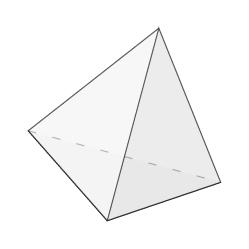
\begin{tikzpicture}
		\coordinate (pic) at (0,0);
		\begin{scope}[shift=(pic), scale=0.8, rotate=-15]
			\coordinate (T) at (pic);
			\coordinate (A) at (-4.5em, -6em);
			\coordinate (B) at (4.5em, -6em);
			\coordinate (C) at (0, -9em);
		\end{scope}
		\draw[fill=gray!10, opacity=0.6] (A) -- (C) -- (B);	% Bottom face
		\draw[loosely dashed, opacity=0.6] (A) -- (B);
		\draw[fill=gray!10, opacity=0.6] (T) -- (A) -- (C);	% Left face
		\draw[fill=gray!25, opacity=0.6] (T) -- (B) -- (C) --cycle;	% Right face
	\end{tikzpicture} \qquad 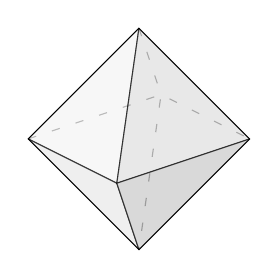
\begin{tikzpicture}
		\coordinate (pic) at (0,0);
		\begin{scope}[shift=(pic), scale=0.8]
			\coordinate (A1) at (pic);
			\coordinate (A2) at (6em, 2em);
			\coordinate (A3) at (10em, 0);
			\coordinate (A4) at (4em, -2em);
			\coordinate (B1) at (5em, 5em);
			\coordinate (B2) at (5em, -5em);
		\end{scope}
		
		\begin{scope}[loosely dashed, opacity=0.6]
			\draw (A1) -- (A2) -- (A3);
			\draw (B1) -- (A2) -- (B2);
		\end{scope}
		\draw[fill=gray!10,opacity=0.6] (A1) -- (A4) -- (B1);
		\draw[fill=gray!20,opacity=0.6] (A1) -- (A4) -- (B2);
		\draw[fill=gray!30,opacity=0.6] (A3) -- (A4) -- (B1);
		\draw[fill=gray!50,opacity=0.6] (A3) -- (A4) -- (B2);
		\draw (B1) -- (A1) -- (B2) -- (A3) --cycle;
	\end{tikzpicture}\end{center}
	等等. 能经由一连串平移, 镜射和旋转而叠合的两个多面体称为全等的, 我们今后仅在全等意义下考察多面体. 其严格定义则是凸分析的内容.
	
	若两个多面体 $P, P'$ 能各自剖分成同样多份较小的多面体 (比方用平面切割)
	\[ P = P_1 \cup \ldots \cup P_r, \quad P' = P'_1 \cup \cdots \cup P'_r \]
	使得对每个 $P_i$ 皆全等于 $P'_i$, 则称 $P$ 和 $P'$ 是剖分全等的. 按常理, 任何关于多面体体积的合理概念都应当在剖分全等下不变; 对于二维空间 $\mathbb{E}^2$ 自然也有相应的定义. 为了研究多面体的体积, Euclid 在《几何原本》卷 XI 运用了所谓的 Eudoxus 穷竭法, 这是现代极限概念的先声. 包括 Gauss 在内的许多数学家对此不甚满意, 他们问: 是否能用初等的剖分方法来判定两个多面体有相同体积? 二维情形的答案是肯定的 (Bolyai--Gerwien 定理, 见 \cite[Theorem 24.7]{Har00}), 三维情形则是 Hilbert 在 1900 年世界数学家大会上提出的问题之一. 以下勾勒 M.\ Dehn 对此的否证.
		\begin{enumerate}[(i)]
			\item 对于多面体 $P$ 的棱 $E$, 记其长度为 $\ell(E) \in \R$, 而其二面角 $\angle E \in \R/\pi\Z$ 定义如下: 任取过 $E$ 内部一点 $x$ 并与 $E$ 垂直的平面 $L$, 计算多边形 $L \cap P$ 在顶点 $x$ 处的内角即是 $\angle E$. 定义 $P$ 的 Dehn 不变量为
				\[ \delta(P) := \sum_{E: \text{棱}} \ell(E) \otimes \angle E \quad \in A. \]
				% Picture
				证明任意立方体的 $\delta$ 为 $0$. 证明棱长为 $\ell$ 的正四面体的 $\delta$ 为 $6\ell \otimes \arccos(\frac{1}{3})$.
			\item 证明若空间中某一平面 $\alpha=0$ 将多面体 $P$ 切成两份 $P = P_+ \cup P_-$, 这里 $P_{\pm} := P \cap \{\pm\alpha \geq 0 \}$, 则 $\delta(P) = \delta(P_+) + \delta(P_-)$. 所以 Dehn 不变量在剖分全等下保持不变.
				\begin{hint}
					讨论平面 $\alpha=0$ 截出的新棱, 典型状况含以下几种
					\begin{center}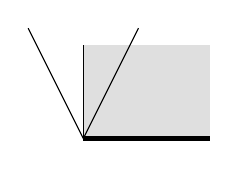
\begin{tikzpicture}[scale=0.7]
						\fill[gray!25] (0,0) rectangle (2.3, 1.7);
						\draw (0,0) -- (-1,2); \draw (0,0) -- (1,2); \draw[ultra thick] (0,0) -- (2.3, 0);
						\draw (0,0) -- (0,1.7);
					\end{tikzpicture} \qquad 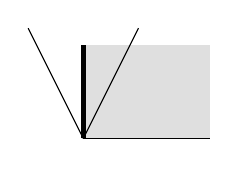
\begin{tikzpicture}[scale=0.7]
						\fill[gray!25] (0,0) rectangle (2.3, 1.7);
						\draw (0,0) -- (-1,2); \draw (0,0) -- (1,2); \draw (0,0) -- (2.3, 0);
						\draw[ultra thick] (0,0) -- (0,1.7);
					\end{tikzpicture} \\ \vspace{2em}
					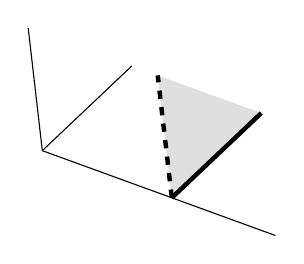
\begin{tikzpicture}[scale=0.7, rotate=-20]
						\fill[gray!25] (0,0) -- (1,2) -- (-1,2) --cycle;
						\draw (-2.5, 0) -- (2, 0);
						\draw[ultra thick] (0,0) -- (1,2); \draw[dashed, ultra thick] (0,0) -- (-1,2);
						\draw (-2.5,0) -- (-3.5, 2); \draw (-2.5,0) -- (-1.5, 2);
					\end{tikzpicture} \qquad 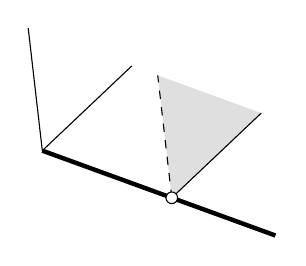
\begin{tikzpicture}[scale=0.7, rotate=-20]
						\fill[gray!25] (0,0) -- (1,2) -- (-1,2) --cycle;
						\draw (0,0) -- (1,2); \draw[dashed] (0,0) -- (-1,2);
						\draw[ultra thick] (0,0) -- (-2.5,0); \draw[ultra thick] (0,0) -- (2,0);
						\filldraw[fill=white] (0,0) circle[radius=3pt];
						\draw (-2.5,0) -- (-3.5, 2); \draw (-2.5,0) -- (-1.5, 2);
					\end{tikzpicture}\end{center}
					其中粗线代表所考虑的新棱, 阴影是平面截出的部分. 以张量积的性质导出 $\delta(P) = \delta(P_+) + \delta(P_-)$.
				\end{hint}
			\item 证明正四面体不可能与立方体剖分全等, 尽管它们的体积可以相同. \hint{问题归结为 $\arccos(\frac{1}{3}) \notin \Q\pi$. 读者可尝试直接论证, 或承认之后的命题 \ref{prop:cos-rationality}.}
		\end{enumerate}
		注记: J.-P.\ Sydler (1965) 证明了 $\mathbb{E}^3$ 中两个多面体 $P, P'$ 剖分全等当且仅当它们有相同的体积与 Dehn 不变量.
	\item 证明推论 \ref{prop:finite-duality} 的构造 $A \mapsto A^\vee$ 给出从有限交换群范畴 $\cate{FinAb}$ 到 $\cate{FinAb}^\text{op}$ 的等价, 并说明它是正合函子.
	\item 对于具有指数的交换群 $A$, 证明 \eqref{eqn:ab-group-duality} 的同态 $\iota_A$ 是单射.
		\begin{hint} 容易处理循环群的情形, 利用 $\Q/\Z$ 是可除 $\Z$-模的性质以过渡到一般情况. \end{hint}
	\item 用图追踪完成命题 \ref{prop:5-lemma-mod} 的证明.
\end{Exercises}
